\batchmode
\documentclass[a4paper]{book}
\usepackage{makeidx}
\usepackage{natbib}
\usepackage{graphicx}
\usepackage{multicol}
\usepackage{float}
\usepackage{listings}
\usepackage{color}
\usepackage{ifthen}
\usepackage[table]{xcolor}
\usepackage{textcomp}
\usepackage{alltt}
\usepackage[utf8]{inputenc}
\usepackage{mathptmx}
\usepackage[scaled=.90]{helvet}
\usepackage{courier}
\usepackage{sectsty}
\usepackage[titles]{tocloft}
\usepackage{doxygen}
\lstset{language=C++,inputencoding=utf8,basicstyle=\footnotesize,breaklines=true,breakatwhitespace=true,tabsize=8,numbers=left }
\makeindex
\setcounter{tocdepth}{3}
\renewcommand{\footrulewidth}{0.4pt}
\renewcommand{\familydefault}{\sfdefault}
\hfuzz=15pt
\setlength{\emergencystretch}{15pt}
\hbadness=750
\tolerance=750
\begin{document}
\begin{titlepage}
\vspace*{7cm}
\begin{center}
{\Large neuro\-\_\-recv }\\
\vspace*{1cm}
{\large \-Generated by Doxygen 1.7.6.1}\\
\vspace*{0.5cm}
{\small Thu Feb 7 2013 12:53:44}\\
\end{center}
\end{titlepage}
\clearemptydoublepage
\pagenumbering{roman}
\tableofcontents
\clearemptydoublepage
\pagenumbering{arabic}
\chapter{\-Main \-Page}
\label{index}

{\bfseries arm} is a \-R\-O\-S package for controlling a \-Manus \-A\-R\-M. \-The package consists of one control node and two teleop nodes. \-You must have a \-Manus \-A\-R\-M properly connected and configured in order for this package to be of any use. \-You must have both a teleop node and the control node running in order to move the \-A\-R\-M. \-There is a node for keyboard teleop and a node for neuron dish activity teleop.\section{\-Code A\-P\-I}\label{index_codeapi}

\begin{DoxyItemize}
\item \-Start the \-A\-R\-M control node by creating an \doxyref{\-Arm\-Control}{p.}{classArmControl} object.
\item \-Start the dish teleop node by creating a \doxyref{\-Teleop\-Arm\-Dish}{p.}{classTeleopArmDish} object.
\item \-Start the keyboard teleop node by creating a \doxyref{\-Teleop\-Arm\-Key}{p.}{classTeleopArmKey} object.
\end{DoxyItemize}


\begin{DoxyItemize}
\item \-To get an instance of the \-A\-R\-M\-: \doxyref{\-Manus\-Arm\-::instance}{p.}{classManusArm_a70516aaf8fa75276f7bb7bcd1912671c}
\item \-To init the \-A\-R\-M\-: \doxyref{\-Manus\-Arm\-::init}{p.}{classManusArm_aeb2e212f64c683e45a6f5bb90afb1a70}
\item \-To move the \-A\-R\-M\-: \doxyref{\-Manus\-Arm\-::move\-Cartesian}{p.}{classManusArm_a66cd2a077fbcdc00d19c76677c900380} and \doxyref{\-Manus\-Arm\-::move\-Constant}{p.}{classManusArm_ab76c4573bfc84e4ce5fe2ad36a8b2522}
\item \-To check if cartesian movement is finished\-: \doxyref{\-Manus\-Arm\-::is\-Move\-Complete}{p.}{classManusArm_a1cff3017b09dfaace5f2c9ca4844d21e}
\item \-To end cartesian movement early\-: \doxyref{\-Manus\-Arm\-::set\-Move\-Complete}{p.}{classManusArm_a4369585e90bd37e57dab71c0e7771d8a}
\item \-To fold/unfold\-: \doxyref{\-Manus\-Arm\-::fold}{p.}{classManusArm_a379092d8f07c767962911d2a410d9d63} and \doxyref{\-Manus\-Arm\-::unfold}{p.}{classManusArm_a29b633fe436ba500058634b8e0a029e5}
\item \-To get joint positions\-: \doxyref{\-Manus\-Arm\-::get\-Print\-State}{p.}{classManusArm_ac6fa919efbacf860202362c1b3611f48} and \doxyref{\-Manus\-Arm\-::get\-Csv\-State}{p.}{classManusArm_a7584b3f88ddc538a8308d7bb7ff1fb89}
\end{DoxyItemize}\section{\-R\-O\-S A\-P\-I}\label{index_rosapi}
\-List of nodes\-:
\begin{DoxyItemize}
\item {\bfseries arm\-\_\-control} 
\item {\bfseries teleop\-\_\-arm\-\_\-dish} 
\item {\bfseries teleop\-\_\-arm\-\_\-key} 
\end{DoxyItemize}



\subsection{arm\-\_\-control}\label{index_arm_control}
arm\-\_\-control controls the \-A\-R\-M. \-It receives movement commands from teleop nodes and moves the arm hardware appropriately.\subsubsection{\-Usage}\label{index_Usage}
\begin{DoxyVerb}
$ rosrun arm arm_control
\end{DoxyVerb}
\subsubsection{\-R\-O\-S topics}\label{index_topics}
\-Subscribes to\-:
\begin{DoxyItemize}
\item {\bfseries \char`\"{}cartesian\-\_\-moves\char`\"{}}\-: [arm/cartesian\-\_\-moves] cartesian movement commands
\item {\bfseries \char`\"{}constant\-\_\-moves\char`\"{}}\-: [arm/constant\-\_\-move] constant movement commands
\item {\bfseries \char`\"{}constant\-\_\-move\-\_\-times\char`\"{}}\-: [arm/constant\-\_\-move\-\_\-time] constant movement by time commands
\end{DoxyItemize}

\-Publishes to\-:
\begin{DoxyItemize}
\item {\bfseries \-N/\-A} 
\end{DoxyItemize}\subsubsection{\-R\-O\-S parameters}\label{index_parameters}
\-Reads the following parameters from the parameter server


\begin{DoxyItemize}
\item {\bfseries \-N/\-A} 
\end{DoxyItemize}

\-Sets the following parameters on the parameter server


\begin{DoxyItemize}
\item {\bfseries \-N/\-A} 
\end{DoxyItemize}\subsubsection{\-R\-O\-S services}\label{index_services}

\begin{DoxyItemize}
\item {\bfseries \char`\"{}time\-\_\-service\char`\"{}}\-: [time\-\_\-server/time\-\_\-srv] polls system time to keep the node in sync
\end{DoxyItemize}



\subsection{teleop\-\_\-arm\-\_\-dish}\label{index_teleop_arm_dish}
teleop\-\_\-arm\-\_\-dish creates movement commands for the arm based on \-C\-A\-T (center of activity trajectory) data received from the \-C\-A\-T creator node.\subsubsection{\-Usage}\label{index_Usage}
\begin{DoxyVerb}
$ rosrun arm teleop_arm_dish
\end{DoxyVerb}
\subsubsection{\-R\-O\-S topics}\label{index_topics}
\-Subscribes to\-:
\begin{DoxyItemize}
\item {\bfseries \char`\"{}cats\char`\"{}}\-: [burst\-\_\-calc/cat] center of activity trajectories
\end{DoxyItemize}

\-Publishes to\-:
\begin{DoxyItemize}
\item {\bfseries \char`\"{}cartesian\-\_\-moves\char`\"{}}\-: [arm/cartesian\-\_\-moves] cartesian movement commands
\item {\bfseries \char`\"{}constant\-\_\-move\-\_\-times\char`\"{}}\-: [arm/constant\-\_\-move\-\_\-time] constant movement by time commands
\end{DoxyItemize}\subsubsection{\-R\-O\-S parameters}\label{index_parameters}
\-Reads the following parameters from the parameter server


\begin{DoxyItemize}
\item {\bfseries arm\-\_\-speed} 
\item {\bfseries arm\-\_\-safe\-\_\-range} 
\item {\bfseries max\-\_\-range\-\_\-from\-\_\-midpoint} 
\end{DoxyItemize}

\-Sets the following parameters on the parameter server


\begin{DoxyItemize}
\item {\bfseries \-N/\-A} 
\end{DoxyItemize}\subsubsection{\-R\-O\-S services}\label{index_services}

\begin{DoxyItemize}
\item {\bfseries \char`\"{}time\-\_\-service\char`\"{}}\-: [time\-\_\-server/time\-\_\-srv] polls system time to keep the node in sync
\end{DoxyItemize}



\subsection{teleop\-\_\-arm\-\_\-key}\label{index_teleop_arm_key}
teleop\-\_\-arm\-\_\-key creates movement commands for the arm based on keyboard input.\subsubsection{\-Usage}\label{index_Usage}
\begin{DoxyVerb}
$ rosrun arm teleop_arm_key
\end{DoxyVerb}
\subsubsection{\-R\-O\-S topics}\label{index_topics}
\-Subscribes to\-:
\begin{DoxyItemize}
\item {\bfseries \-N/\-A} 
\end{DoxyItemize}

\-Publishes to\-:
\begin{DoxyItemize}
\item {\bfseries \char`\"{}constant\-\_\-moves\char`\"{}}\-: [arm/constant\-\_\-move] constant movement commands
\end{DoxyItemize}\subsubsection{\-R\-O\-S parameters}\label{index_parameters}
\-Reads the following parameters from the parameter server


\begin{DoxyItemize}
\item {\bfseries \-N/\-A} 
\end{DoxyItemize}

\-Sets the following parameters on the parameter server


\begin{DoxyItemize}
\item {\bfseries \-N/\-A} 
\end{DoxyItemize}\subsubsection{\-R\-O\-S services}\label{index_services}

\begin{DoxyItemize}
\item {\bfseries \-N/\-A} 
\end{DoxyItemize}\section{\-Command-\/line tools}\label{index_commandline}
\-There are several launch files available to simplify running all of the nodes. \-Each launch file has a corresponding parameter file. \-They are as follows\-:


\begin{DoxyItemize}
\item brian\-\_\-csv.\-launch
\item brian\-\_\-sim.\-launch
\item csv.\-launch
\item volt\-\_\-only\-\_\-brian\-\_\-csv.\-launch
\item volt\-\_\-only\-\_\-brian\-\_\-sim.\-launch
\item volt\-\_\-only\-\_\-csv.\-launch
\end{DoxyItemize}\subsection{\-Usage}\label{index_Usage}
\begin{DoxyVerb}
$ roslaunch [package] [file]
\end{DoxyVerb}


\begin{DoxyParagraph}{\-Example}

\end{DoxyParagraph}
\begin{DoxyVerb}
$ roslaunch arm csv.launch
\end{DoxyVerb}
 
\chapter{\-Namespace \-Index}
\section{\-Namespace \-List}
\-Here is a list of all namespaces with brief descriptions\-:\begin{DoxyCompactList}
\item\contentsline{section}{{\bf burst\-\_\-calc} }{\pageref{namespaceburst__calc}}{}
\item\contentsline{section}{{\bf burst\-\_\-calc\-::msg} }{\pageref{namespaceburst__calc_1_1msg}}{}
\item\contentsline{section}{{\bf burst\-\_\-calc\-::msg\-::\-\_\-burst} }{\pageref{namespaceburst__calc_1_1msg_1_1__burst}}{}
\item\contentsline{section}{{\bf burst\-\_\-calc\-::msg\-::\-\_\-ca} }{\pageref{namespaceburst__calc_1_1msg_1_1__ca}}{}
\item\contentsline{section}{{\bf burst\-\_\-calc\-::msg\-::\-\_\-cat} }{\pageref{namespaceburst__calc_1_1msg_1_1__cat}}{}
\item\contentsline{section}{{\bf burst\-\_\-calc\-::msg\-::\-\_\-ranges} }{\pageref{namespaceburst__calc_1_1msg_1_1__ranges}}{}
\item\contentsline{section}{{\bf ros} }{\pageref{namespaceros}}{}
\item\contentsline{section}{{\bf ros\-::message\-\_\-operations} }{\pageref{namespaceros_1_1message__operations}}{}
\item\contentsline{section}{{\bf ros\-::message\-\_\-traits} }{\pageref{namespaceros_1_1message__traits}}{}
\item\contentsline{section}{{\bf ros\-::serialization} }{\pageref{namespaceros_1_1serialization}}{}
\end{DoxyCompactList}

\chapter{\-Class \-Index}
\section{\-Class \-List}
\-Here are the classes, structs, unions and interfaces with brief descriptions\-:\begin{DoxyCompactList}
\item\contentsline{section}{{\bf \-Arm\-Control} \\*\-Node for controlling the \-A\-R\-M }{\pageref{classArmControl}}{}
\item\contentsline{section}{{\bf \-Arm\-Exception} }{\pageref{classArmException}}{}
\item\contentsline{section}{{\bf arm\-State} \\*\-Stores \-A\-R\-M state }{\pageref{structarmState}}{}
\item\contentsline{section}{{\bf arm.\-msg.\-\_\-cartesian\-\_\-move.\-cartesian\-\_\-move} }{\pageref{classarm_1_1msg_1_1__cartesian__move_1_1cartesian__move}}{}
\item\contentsline{section}{{\bf arm\-::cartesian\-\_\-move\-\_\-$<$ Container\-Allocator $>$} }{\pageref{structarm_1_1cartesian__move__}}{}
\item\contentsline{section}{{\bf arm.\-msg.\-\_\-cartesian\-\_\-moves.\-cartesian\-\_\-moves} }{\pageref{classarm_1_1msg_1_1__cartesian__moves_1_1cartesian__moves}}{}
\item\contentsline{section}{{\bf arm\-::cartesian\-\_\-moves\-\_\-$<$ Container\-Allocator $>$} }{\pageref{structarm_1_1cartesian__moves__}}{}
\item\contentsline{section}{{\bf \-Cartesian\-Move} \\*\-Struct for holding \-Cartesian movement data }{\pageref{structCartesianMove}}{}
\item\contentsline{section}{{\bf arm.\-msg.\-\_\-constant\-\_\-move.\-constant\-\_\-move} }{\pageref{classarm_1_1msg_1_1__constant__move_1_1constant__move}}{}
\item\contentsline{section}{{\bf arm\-::constant\-\_\-move\-\_\-$<$ Container\-Allocator $>$} }{\pageref{structarm_1_1constant__move__}}{}
\item\contentsline{section}{{\bf arm.\-msg.\-\_\-constant\-\_\-move\-\_\-time.\-constant\-\_\-move\-\_\-time} }{\pageref{classarm_1_1msg_1_1__constant__move__time_1_1constant__move__time}}{}
\item\contentsline{section}{{\bf arm\-::constant\-\_\-move\-\_\-time\-\_\-$<$ Container\-Allocator $>$} }{\pageref{structarm_1_1constant__move__time__}}{}
\item\contentsline{section}{{\bf \-Constant\-Move} \\*\-Struct for holding constant movement data }{\pageref{structConstantMove}}{}
\item\contentsline{section}{{\bf ros\-::message\-\_\-traits\-::\-Data\-Type$<$ \-::arm\-::cartesian\-\_\-move\-\_\-$<$ Container\-Allocator $>$ $>$} }{\pageref{structros_1_1message__traits_1_1DataType_3_01_1_1arm_1_1cartesian__move___3_01ContainerAllocator_01_4_01_4}}{}
\item\contentsline{section}{{\bf ros\-::message\-\_\-traits\-::\-Data\-Type$<$ \-::arm\-::cartesian\-\_\-moves\-\_\-$<$ Container\-Allocator $>$ $>$} }{\pageref{structros_1_1message__traits_1_1DataType_3_01_1_1arm_1_1cartesian__moves___3_01ContainerAllocator_01_4_01_4}}{}
\item\contentsline{section}{{\bf ros\-::message\-\_\-traits\-::\-Data\-Type$<$ \-::arm\-::constant\-\_\-move\-\_\-$<$ Container\-Allocator $>$ $>$} }{\pageref{structros_1_1message__traits_1_1DataType_3_01_1_1arm_1_1constant__move___3_01ContainerAllocator_01_4_01_4}}{}
\item\contentsline{section}{{\bf ros\-::message\-\_\-traits\-::\-Data\-Type$<$ \-::arm\-::constant\-\_\-move\-\_\-time\-\_\-$<$ Container\-Allocator $>$ $>$} }{\pageref{structros_1_1message__traits_1_1DataType_3_01_1_1arm_1_1constant__move__time___3_01ContainerAllocator_01_4_01_4}}{}
\item\contentsline{section}{{\bf ros\-::message\-\_\-traits\-::\-Definition$<$ \-::arm\-::cartesian\-\_\-move\-\_\-$<$ Container\-Allocator $>$ $>$} }{\pageref{structros_1_1message__traits_1_1Definition_3_01_1_1arm_1_1cartesian__move___3_01ContainerAllocator_01_4_01_4}}{}
\item\contentsline{section}{{\bf ros\-::message\-\_\-traits\-::\-Definition$<$ \-::arm\-::cartesian\-\_\-moves\-\_\-$<$ Container\-Allocator $>$ $>$} }{\pageref{structros_1_1message__traits_1_1Definition_3_01_1_1arm_1_1cartesian__moves___3_01ContainerAllocator_01_4_01_4}}{}
\item\contentsline{section}{{\bf ros\-::message\-\_\-traits\-::\-Definition$<$ \-::arm\-::constant\-\_\-move\-\_\-$<$ Container\-Allocator $>$ $>$} }{\pageref{structros_1_1message__traits_1_1Definition_3_01_1_1arm_1_1constant__move___3_01ContainerAllocator_01_4_01_4}}{}
\item\contentsline{section}{{\bf ros\-::message\-\_\-traits\-::\-Definition$<$ \-::arm\-::constant\-\_\-move\-\_\-time\-\_\-$<$ Container\-Allocator $>$ $>$} }{\pageref{structros_1_1message__traits_1_1Definition_3_01_1_1arm_1_1constant__move__time___3_01ContainerAllocator_01_4_01_4}}{}
\item\contentsline{section}{{\bf ros\-::message\-\_\-traits\-::\-Has\-Header$<$ \-::arm\-::cartesian\-\_\-move\-\_\-$<$ Container\-Allocator $>$ $>$} }{\pageref{structros_1_1message__traits_1_1HasHeader_3_01_1_1arm_1_1cartesian__move___3_01ContainerAllocator_01_4_01_4}}{}
\item\contentsline{section}{{\bf ros\-::message\-\_\-traits\-::\-Has\-Header$<$ \-::arm\-::cartesian\-\_\-moves\-\_\-$<$ Container\-Allocator $>$ $>$} }{\pageref{structros_1_1message__traits_1_1HasHeader_3_01_1_1arm_1_1cartesian__moves___3_01ContainerAllocator_01_4_01_4}}{}
\item\contentsline{section}{{\bf ros\-::message\-\_\-traits\-::\-Has\-Header$<$ \-::arm\-::constant\-\_\-move\-\_\-$<$ Container\-Allocator $>$ $>$} }{\pageref{structros_1_1message__traits_1_1HasHeader_3_01_1_1arm_1_1constant__move___3_01ContainerAllocator_01_4_01_4}}{}
\item\contentsline{section}{{\bf ros\-::message\-\_\-traits\-::\-Has\-Header$<$ \-::arm\-::constant\-\_\-move\-\_\-time\-\_\-$<$ Container\-Allocator $>$ $>$} }{\pageref{structros_1_1message__traits_1_1HasHeader_3_01_1_1arm_1_1constant__move__time___3_01ContainerAllocator_01_4_01_4}}{}
\item\contentsline{section}{{\bf ros\-::message\-\_\-traits\-::\-Has\-Header$<$ const \-::arm\-::cartesian\-\_\-move\-\_\-$<$ Container\-Allocator $>$ $>$} }{\pageref{structros_1_1message__traits_1_1HasHeader_3_01const_01_1_1arm_1_1cartesian__move___3_01ContainerAllocator_01_4_01_4}}{}
\item\contentsline{section}{{\bf ros\-::message\-\_\-traits\-::\-Has\-Header$<$ const \-::arm\-::cartesian\-\_\-moves\-\_\-$<$ Container\-Allocator $>$ $>$} }{\pageref{structros_1_1message__traits_1_1HasHeader_3_01const_01_1_1arm_1_1cartesian__moves___3_01ContainerAllocator_01_4_01_4}}{}
\item\contentsline{section}{{\bf ros\-::message\-\_\-traits\-::\-Has\-Header$<$ const \-::arm\-::constant\-\_\-move\-\_\-$<$ Container\-Allocator $>$ $>$} }{\pageref{structros_1_1message__traits_1_1HasHeader_3_01const_01_1_1arm_1_1constant__move___3_01ContainerAllocator_01_4_01_4}}{}
\item\contentsline{section}{{\bf ros\-::message\-\_\-traits\-::\-Has\-Header$<$ const \-::arm\-::constant\-\_\-move\-\_\-time\-\_\-$<$ Container\-Allocator $>$ $>$} }{\pageref{structros_1_1message__traits_1_1HasHeader_3_01const_01_1_1arm_1_1constant__move__time___3_01ContainerAllocator_01_4_01_4}}{}
\item\contentsline{section}{{\bf ros\-::message\-\_\-traits\-::\-Is\-Message$<$ \-::arm\-::cartesian\-\_\-move\-\_\-$<$ Container\-Allocator $>$ $>$} }{\pageref{structros_1_1message__traits_1_1IsMessage_3_01_1_1arm_1_1cartesian__move___3_01ContainerAllocator_01_4_01_4}}{}
\item\contentsline{section}{{\bf ros\-::message\-\_\-traits\-::\-Is\-Message$<$ \-::arm\-::cartesian\-\_\-move\-\_\-$<$ Container\-Allocator $>$const  $>$} }{\pageref{structros_1_1message__traits_1_1IsMessage_3_01_1_1arm_1_1cartesian__move___3_01ContainerAllocator_01_4const_01_01_4}}{}
\item\contentsline{section}{{\bf ros\-::message\-\_\-traits\-::\-Is\-Message$<$ \-::arm\-::cartesian\-\_\-moves\-\_\-$<$ Container\-Allocator $>$ $>$} }{\pageref{structros_1_1message__traits_1_1IsMessage_3_01_1_1arm_1_1cartesian__moves___3_01ContainerAllocator_01_4_01_4}}{}
\item\contentsline{section}{{\bf ros\-::message\-\_\-traits\-::\-Is\-Message$<$ \-::arm\-::cartesian\-\_\-moves\-\_\-$<$ Container\-Allocator $>$const  $>$} }{\pageref{structros_1_1message__traits_1_1IsMessage_3_01_1_1arm_1_1cartesian__moves___3_01ContainerAllocator_01_4const_01_01_4}}{}
\item\contentsline{section}{{\bf ros\-::message\-\_\-traits\-::\-Is\-Message$<$ \-::arm\-::constant\-\_\-move\-\_\-$<$ Container\-Allocator $>$ $>$} }{\pageref{structros_1_1message__traits_1_1IsMessage_3_01_1_1arm_1_1constant__move___3_01ContainerAllocator_01_4_01_4}}{}
\item\contentsline{section}{{\bf ros\-::message\-\_\-traits\-::\-Is\-Message$<$ \-::arm\-::constant\-\_\-move\-\_\-$<$ Container\-Allocator $>$const  $>$} }{\pageref{structros_1_1message__traits_1_1IsMessage_3_01_1_1arm_1_1constant__move___3_01ContainerAllocator_01_4const_01_01_4}}{}
\item\contentsline{section}{{\bf ros\-::message\-\_\-traits\-::\-Is\-Message$<$ \-::arm\-::constant\-\_\-move\-\_\-time\-\_\-$<$ Container\-Allocator $>$ $>$} }{\pageref{structros_1_1message__traits_1_1IsMessage_3_01_1_1arm_1_1constant__move__time___3_01ContainerAllocator_01_4_01_4}}{}
\item\contentsline{section}{{\bf ros\-::message\-\_\-traits\-::\-Is\-Message$<$ \-::arm\-::constant\-\_\-move\-\_\-time\-\_\-$<$ Container\-Allocator $>$const  $>$} }{\pageref{structros_1_1message__traits_1_1IsMessage_3_01_1_1arm_1_1constant__move__time___3_01ContainerAllocator_01_4const_01_01_4}}{}
\item\contentsline{section}{{\bf \-Manus\-Arm} \\*\-Singleton class representing the \-A\-R\-M. \begin{DoxyCopyright}{\-Copyright}
\-Copyright 2013 \-University of \-Massachusetts \-Lowell 
\end{DoxyCopyright}
}{\pageref{classManusArm}}{}
\item\contentsline{section}{{\bf ros\-::message\-\_\-traits\-::\-M\-D5\-Sum$<$ \-::arm\-::cartesian\-\_\-move\-\_\-$<$ Container\-Allocator $>$ $>$} }{\pageref{structros_1_1message__traits_1_1MD5Sum_3_01_1_1arm_1_1cartesian__move___3_01ContainerAllocator_01_4_01_4}}{}
\item\contentsline{section}{{\bf ros\-::message\-\_\-traits\-::\-M\-D5\-Sum$<$ \-::arm\-::cartesian\-\_\-moves\-\_\-$<$ Container\-Allocator $>$ $>$} }{\pageref{structros_1_1message__traits_1_1MD5Sum_3_01_1_1arm_1_1cartesian__moves___3_01ContainerAllocator_01_4_01_4}}{}
\item\contentsline{section}{{\bf ros\-::message\-\_\-traits\-::\-M\-D5\-Sum$<$ \-::arm\-::constant\-\_\-move\-\_\-$<$ Container\-Allocator $>$ $>$} }{\pageref{structros_1_1message__traits_1_1MD5Sum_3_01_1_1arm_1_1constant__move___3_01ContainerAllocator_01_4_01_4}}{}
\item\contentsline{section}{{\bf ros\-::message\-\_\-traits\-::\-M\-D5\-Sum$<$ \-::arm\-::constant\-\_\-move\-\_\-time\-\_\-$<$ Container\-Allocator $>$ $>$} }{\pageref{structros_1_1message__traits_1_1MD5Sum_3_01_1_1arm_1_1constant__move__time___3_01ContainerAllocator_01_4_01_4}}{}
\item\contentsline{section}{{\bf ros\-::message\-\_\-operations\-::\-Printer$<$ \-::arm\-::cartesian\-\_\-move\-\_\-$<$ Container\-Allocator $>$ $>$} }{\pageref{structros_1_1message__operations_1_1Printer_3_01_1_1arm_1_1cartesian__move___3_01ContainerAllocator_01_4_01_4}}{}
\item\contentsline{section}{{\bf ros\-::message\-\_\-operations\-::\-Printer$<$ \-::arm\-::cartesian\-\_\-moves\-\_\-$<$ Container\-Allocator $>$ $>$} }{\pageref{structros_1_1message__operations_1_1Printer_3_01_1_1arm_1_1cartesian__moves___3_01ContainerAllocator_01_4_01_4}}{}
\item\contentsline{section}{{\bf ros\-::message\-\_\-operations\-::\-Printer$<$ \-::arm\-::constant\-\_\-move\-\_\-$<$ Container\-Allocator $>$ $>$} }{\pageref{structros_1_1message__operations_1_1Printer_3_01_1_1arm_1_1constant__move___3_01ContainerAllocator_01_4_01_4}}{}
\item\contentsline{section}{{\bf ros\-::message\-\_\-operations\-::\-Printer$<$ \-::arm\-::constant\-\_\-move\-\_\-time\-\_\-$<$ Container\-Allocator $>$ $>$} }{\pageref{structros_1_1message__operations_1_1Printer_3_01_1_1arm_1_1constant__move__time___3_01ContainerAllocator_01_4_01_4}}{}
\item\contentsline{section}{{\bf ros\-::serialization\-::\-Serializer$<$ \-::arm\-::cartesian\-\_\-move\-\_\-$<$ Container\-Allocator $>$ $>$} }{\pageref{structros_1_1serialization_1_1Serializer_3_01_1_1arm_1_1cartesian__move___3_01ContainerAllocator_01_4_01_4}}{}
\item\contentsline{section}{{\bf ros\-::serialization\-::\-Serializer$<$ \-::arm\-::cartesian\-\_\-moves\-\_\-$<$ Container\-Allocator $>$ $>$} }{\pageref{structros_1_1serialization_1_1Serializer_3_01_1_1arm_1_1cartesian__moves___3_01ContainerAllocator_01_4_01_4}}{}
\item\contentsline{section}{{\bf ros\-::serialization\-::\-Serializer$<$ \-::arm\-::constant\-\_\-move\-\_\-$<$ Container\-Allocator $>$ $>$} }{\pageref{structros_1_1serialization_1_1Serializer_3_01_1_1arm_1_1constant__move___3_01ContainerAllocator_01_4_01_4}}{}
\item\contentsline{section}{{\bf ros\-::serialization\-::\-Serializer$<$ \-::arm\-::constant\-\_\-move\-\_\-time\-\_\-$<$ Container\-Allocator $>$ $>$} }{\pageref{structros_1_1serialization_1_1Serializer_3_01_1_1arm_1_1constant__move__time___3_01ContainerAllocator_01_4_01_4}}{}
\item\contentsline{section}{{\bf \-Teleop\-Arm\-Dish} \\*\-Node for \-A\-R\-M teleop from the neuron dish }{\pageref{classTeleopArmDish}}{}
\item\contentsline{section}{{\bf \-Teleop\-Arm\-Key} \\*\-Node for \-A\-R\-M teleop from the keyboard }{\pageref{classTeleopArmKey}}{}
\end{DoxyCompactList}

\chapter{\-File \-Index}
\section{\-File \-List}
\-Here is a list of all files with brief descriptions\-:\begin{DoxyCompactList}
\item\contentsline{section}{{\bf \-\_\-\-\_\-init\-\_\-\-\_\-.\-py} }{\pageref{____init_____8py}}{}
\item\contentsline{section}{{\bf msg/\-\_\-\-\_\-init\-\_\-\-\_\-.\-py} }{\pageref{msg_2____init_____8py}}{}
\item\contentsline{section}{{\bf \-\_\-dish\-\_\-state.\-py} }{\pageref{__dish__state_8py}}{}
\item\contentsline{section}{{\bf brian\-\_\-recv.\-py} }{\pageref{brian__recv_8py}}{}
\item\contentsline{section}{{\bf brian\-\_\-to\-\_\-csv.\-py} }{\pageref{brian__to__csv_8py}}{}
\item\contentsline{section}{{\bf csv\-\_\-recv.\-cpp} }{\pageref{csv__recv_8cpp}}{}
\item\contentsline{section}{{\bf csv\-\_\-recv.\-h} }{\pageref{csv__recv_8h}}{}
\item\contentsline{section}{{\bf dish\-\_\-generator.\-cpp} }{\pageref{dish__generator_8cpp}}{}
\item\contentsline{section}{{\bf dish\-\_\-state.\-h} }{\pageref{dish__state_8h}}{}
\item\contentsline{section}{{\bf \-Seed\-Mea.\-py} }{\pageref{SeedMea_8py}}{}
\end{DoxyCompactList}

\chapter{\-Namespace \-Documentation}
\section{brian\-\_\-recv \-Namespace \-Reference}
\label{namespacebrian__recv}\index{brian\-\_\-recv@{brian\-\_\-recv}}


\doxyref{brian\-\_\-recv}{p.}{namespacebrian__recv} is a \-R\-O\-S node that runs a \-Brian simulation, then creates and publishes dish\-\_\-states using the generated data.  


\subsection*{\-Classes}
\begin{DoxyCompactItemize}
\item 
class {\bf \-Brian\-Simulation}
\begin{DoxyCompactList}\small\item\em \-Runs a \-Brian simulation, then creates and publishes dish\-\_\-states using the generated data. \end{DoxyCompactList}\item 
class {\bf \-Channel}
\begin{DoxyCompactList}\small\item\em \-Data structure for a multi electrode array channel pad neurons \-: list of neurons within range of the pad total\-\_\-weight \-: combined weights of all the neurons. \end{DoxyCompactList}\item 
class {\bf \-Close\-Neuron}
\begin{DoxyCompactList}\small\item\em \-Data structure representing a neuron that is within range of a channel pad self.\-data \-: unique id of the neuron self.\-weight \-: how much weight this neuron has in calculating average activity for its channel. \end{DoxyCompactList}\end{DoxyCompactItemize}
\subsection*{\-Functions}
\begin{DoxyCompactItemize}
\item 
def {\bf channelizer}
\begin{DoxyCompactList}\small\item\em \-Channelizer takes data from an 8x8 map and populates a 60-\/channel list. \end{DoxyCompactList}\end{DoxyCompactItemize}
\subsection*{\-Variables}
\begin{DoxyCompactItemize}
\item 
tuple {\bf brian} = {\bf \-Brian\-Simulation}({\bf connections}, {\bf channels})
\item 
tuple {\bf channels} = {\bf channelizer}({\bf pad\-\_\-neuron\-\_\-map})
\item 
tuple {\bf connections} = \-Unpickler({\bf connections\-\_\-file})
\item 
tuple {\bf connections\-\_\-file} = open({\bf connections\-\_\-file\-\_\-name})
\item 
tuple {\bf connections\-\_\-file\-\_\-name} = rospy.\-get\-\_\-param('brian\-\_\-connections\-\_\-file\-\_\-path')
\item 
tuple {\bf pad\-\_\-neuron\-\_\-map} = \-Unpickler({\bf pad\-\_\-neuron\-\_\-map\-\_\-file})
\item 
tuple {\bf pad\-\_\-neuron\-\_\-map\-\_\-file} = open({\bf pad\-\_\-neuron\-\_\-map\-\_\-file\-\_\-name})
\item 
tuple {\bf pad\-\_\-neuron\-\_\-map\-\_\-file\-\_\-name} = rospy.\-get\-\_\-param('brian\-\_\-pad\-\_\-neuron\-\_\-map\-\_\-file\-\_\-path')
\end{DoxyCompactItemize}


\subsection{\-Detailed \-Description}
\doxyref{brian\-\_\-recv}{p.}{namespacebrian__recv} is a \-R\-O\-S node that runs a \-Brian simulation, then creates and publishes dish\-\_\-states using the generated data. \-Running network simulations in \-Brian can take quite a while. \-An alternate method is to generate a \-C\-S\-V file using the \doxyref{brian\-\_\-to\-\_\-csv.\-py}{p.}{brian__to__csv_8py} node and then use the csv\-\_\-recv node.

\begin{DoxyCopyright}{\-Copyright}
\-Copyright 2013 \-University of \-Massachusetts \-Lowell 
\end{DoxyCopyright}
\begin{DoxyAuthor}{\-Author}
\-Jonathan \-Hasenzahl 

\-Abraham \-Shultz 
\end{DoxyAuthor}


\subsection{\-Function \-Documentation}
\index{brian\-\_\-recv@{brian\-\_\-recv}!channelizer@{channelizer}}
\index{channelizer@{channelizer}!brian_recv@{brian\-\_\-recv}}
\subsubsection[{channelizer}]{\setlength{\rightskip}{0pt plus 5cm}def {\bf brian\-\_\-recv.\-channelizer} (
\begin{DoxyParamCaption}
\item[{}]{pad\-\_\-neuron\-\_\-map}
\end{DoxyParamCaption}
)}\label{namespacebrian__recv_a19968f912d208f1bab39f4485ec82b98}


\-Channelizer takes data from an 8x8 map and populates a 60-\/channel list. 



\-Definition at line 285 of file brian\-\_\-recv.\-py.



\subsection{\-Variable \-Documentation}
\index{brian\-\_\-recv@{brian\-\_\-recv}!brian@{brian}}
\index{brian@{brian}!brian_recv@{brian\-\_\-recv}}
\subsubsection[{brian}]{\setlength{\rightskip}{0pt plus 5cm}tuple {\bf brian\-\_\-recv\-::brian} = {\bf \-Brian\-Simulation}({\bf connections}, {\bf channels})}\label{namespacebrian__recv_a965f28b945f5c79bdf867fc7e50e53c6}


\-Definition at line 328 of file brian\-\_\-recv.\-py.

\index{brian\-\_\-recv@{brian\-\_\-recv}!channels@{channels}}
\index{channels@{channels}!brian_recv@{brian\-\_\-recv}}
\subsubsection[{channels}]{\setlength{\rightskip}{0pt plus 5cm}tuple {\bf brian\-\_\-recv\-::channels} = {\bf channelizer}({\bf pad\-\_\-neuron\-\_\-map})}\label{namespacebrian__recv_a7be2a6cef1f933aaaf6c7b7e28ad0af6}


\-Definition at line 324 of file brian\-\_\-recv.\-py.

\index{brian\-\_\-recv@{brian\-\_\-recv}!connections@{connections}}
\index{connections@{connections}!brian_recv@{brian\-\_\-recv}}
\subsubsection[{connections}]{\setlength{\rightskip}{0pt plus 5cm}tuple {\bf brian\-\_\-recv\-::connections} = \-Unpickler({\bf connections\-\_\-file})}\label{namespacebrian__recv_ae6df3c8e532f1efc00d9d28c9ae28239}


\-Definition at line 318 of file brian\-\_\-recv.\-py.

\index{brian\-\_\-recv@{brian\-\_\-recv}!connections\-\_\-file@{connections\-\_\-file}}
\index{connections\-\_\-file@{connections\-\_\-file}!brian_recv@{brian\-\_\-recv}}
\subsubsection[{connections\-\_\-file}]{\setlength{\rightskip}{0pt plus 5cm}tuple {\bf brian\-\_\-recv\-::connections\-\_\-file} = open({\bf connections\-\_\-file\-\_\-name})}\label{namespacebrian__recv_a4088f600609b9462003ae30f7b6c5d48}


\-Definition at line 312 of file brian\-\_\-recv.\-py.

\index{brian\-\_\-recv@{brian\-\_\-recv}!connections\-\_\-file\-\_\-name@{connections\-\_\-file\-\_\-name}}
\index{connections\-\_\-file\-\_\-name@{connections\-\_\-file\-\_\-name}!brian_recv@{brian\-\_\-recv}}
\subsubsection[{connections\-\_\-file\-\_\-name}]{\setlength{\rightskip}{0pt plus 5cm}tuple {\bf brian\-\_\-recv\-::connections\-\_\-file\-\_\-name} = rospy.\-get\-\_\-param('brian\-\_\-connections\-\_\-file\-\_\-path')}\label{namespacebrian__recv_aa6339b10cab0182ec7cee3c63631c8e5}


\-Definition at line 305 of file brian\-\_\-recv.\-py.

\index{brian\-\_\-recv@{brian\-\_\-recv}!pad\-\_\-neuron\-\_\-map@{pad\-\_\-neuron\-\_\-map}}
\index{pad\-\_\-neuron\-\_\-map@{pad\-\_\-neuron\-\_\-map}!brian_recv@{brian\-\_\-recv}}
\subsubsection[{pad\-\_\-neuron\-\_\-map}]{\setlength{\rightskip}{0pt plus 5cm}tuple {\bf brian\-\_\-recv\-::pad\-\_\-neuron\-\_\-map} = \-Unpickler({\bf pad\-\_\-neuron\-\_\-map\-\_\-file})}\label{namespacebrian__recv_a5e05e02ee2aae14151515020dc0487a4}


\-Definition at line 319 of file brian\-\_\-recv.\-py.

\index{brian\-\_\-recv@{brian\-\_\-recv}!pad\-\_\-neuron\-\_\-map\-\_\-file@{pad\-\_\-neuron\-\_\-map\-\_\-file}}
\index{pad\-\_\-neuron\-\_\-map\-\_\-file@{pad\-\_\-neuron\-\_\-map\-\_\-file}!brian_recv@{brian\-\_\-recv}}
\subsubsection[{pad\-\_\-neuron\-\_\-map\-\_\-file}]{\setlength{\rightskip}{0pt plus 5cm}tuple {\bf brian\-\_\-recv\-::pad\-\_\-neuron\-\_\-map\-\_\-file} = open({\bf pad\-\_\-neuron\-\_\-map\-\_\-file\-\_\-name})}\label{namespacebrian__recv_aa7f76a598c26ae4dda31ed7d27db533d}


\-Definition at line 313 of file brian\-\_\-recv.\-py.

\index{brian\-\_\-recv@{brian\-\_\-recv}!pad\-\_\-neuron\-\_\-map\-\_\-file\-\_\-name@{pad\-\_\-neuron\-\_\-map\-\_\-file\-\_\-name}}
\index{pad\-\_\-neuron\-\_\-map\-\_\-file\-\_\-name@{pad\-\_\-neuron\-\_\-map\-\_\-file\-\_\-name}!brian_recv@{brian\-\_\-recv}}
\subsubsection[{pad\-\_\-neuron\-\_\-map\-\_\-file\-\_\-name}]{\setlength{\rightskip}{0pt plus 5cm}tuple {\bf brian\-\_\-recv\-::pad\-\_\-neuron\-\_\-map\-\_\-file\-\_\-name} = rospy.\-get\-\_\-param('brian\-\_\-pad\-\_\-neuron\-\_\-map\-\_\-file\-\_\-path')}\label{namespacebrian__recv_ad5b0a11332270ff3ca3de2a11bec9661}


\-Definition at line 306 of file brian\-\_\-recv.\-py.


\section{brian\-\_\-to\-\_\-csv \-Namespace \-Reference}
\label{namespacebrian__to__csv}\index{brian\-\_\-to\-\_\-csv@{brian\-\_\-to\-\_\-csv}}


\-This is a \-R\-O\-S node that is used by itself to generate \-C\-S\-V data files by running \-Brian simulations.  


\subsection*{\-Classes}
\begin{DoxyCompactItemize}
\item 
class {\bf \-Channel}
\begin{DoxyCompactList}\small\item\em structure for a \-M\-E\-A channel pad neurons\-: list of neurons within range of the pad total\-\_\-weight\-: combined weights of all the neurons \end{DoxyCompactList}\item 
class {\bf \-Close\-Neuron}
\begin{DoxyCompactList}\small\item\em \-Data structure for a neuron that is close to a channel pad. \end{DoxyCompactList}\end{DoxyCompactItemize}
\subsection*{\-Functions}
\begin{DoxyCompactItemize}
\item 
def {\bf brian\-Recv}
\begin{DoxyCompactList}\small\item\em \-Runs a \-Brian simulation \char`\"{}\-P\char`\"{} and records and publishes voltages captured by the multielectrode array \char`\"{}channels\char`\"{}. \end{DoxyCompactList}\item 
def {\bf channelizer}
\begin{DoxyCompactList}\small\item\em \-Populates a 60-\/channel list using data from an x,y map. \end{DoxyCompactList}\end{DoxyCompactItemize}
\subsection*{\-Variables}
\begin{DoxyCompactItemize}
\item 
tuple {\bf channels} = {\bf channelizer}({\bf pad\-\_\-neuron\-\_\-map})
\item 
tuple {\bf connections} = \-Unpickler({\bf connections\-\_\-file})
\item 
tuple {\bf connections\-\_\-file} = open({\bf connections\-\_\-file\-\_\-name})
\item 
tuple {\bf connections\-\_\-file\-\_\-name} = rospy.\-get\-\_\-param('brian\-\_\-connections\-\_\-file\-\_\-path')
\item 
tuple {\bf pad\-\_\-neuron\-\_\-map} = \-Unpickler({\bf pad\-\_\-neuron\-\_\-map\-\_\-file})
\item 
tuple {\bf pad\-\_\-neuron\-\_\-map\-\_\-file} = open({\bf pad\-\_\-neuron\-\_\-map\-\_\-file\-\_\-name})
\item 
tuple {\bf pad\-\_\-neuron\-\_\-map\-\_\-file\-\_\-name} = rospy.\-get\-\_\-param('brian\-\_\-pad\-\_\-neuron\-\_\-map\-\_\-file\-\_\-path')
\end{DoxyCompactItemize}


\subsection{\-Detailed \-Description}
\-This is a \-R\-O\-S node that is used by itself to generate \-C\-S\-V data files by running \-Brian simulations. \-Use this node to generate a \-C\-S\-V file, and then use the csv\-\_\-recv node to read the generated file. 

\subsection{\-Function \-Documentation}
\index{brian\-\_\-to\-\_\-csv@{brian\-\_\-to\-\_\-csv}!brian\-Recv@{brian\-Recv}}
\index{brian\-Recv@{brian\-Recv}!brian_to_csv@{brian\-\_\-to\-\_\-csv}}
\subsubsection[{brian\-Recv}]{\setlength{\rightskip}{0pt plus 5cm}def {\bf brian\-\_\-to\-\_\-csv.\-brian\-Recv} (
\begin{DoxyParamCaption}
\item[{}]{connections, }
\item[{}]{channels}
\end{DoxyParamCaption}
)}\label{namespacebrian__to__csv_a353f1ee33c7a0784d4a320f129720691}


\-Runs a \-Brian simulation \char`\"{}\-P\char`\"{} and records and publishes voltages captured by the multielectrode array \char`\"{}channels\char`\"{}. 



\-Definition at line 67 of file brian\-\_\-to\-\_\-csv.\-py.

\index{brian\-\_\-to\-\_\-csv@{brian\-\_\-to\-\_\-csv}!channelizer@{channelizer}}
\index{channelizer@{channelizer}!brian_to_csv@{brian\-\_\-to\-\_\-csv}}
\subsubsection[{channelizer}]{\setlength{\rightskip}{0pt plus 5cm}def {\bf brian\-\_\-to\-\_\-csv.\-channelizer} (
\begin{DoxyParamCaption}
\item[{}]{pad\-\_\-neuron\-\_\-map}
\end{DoxyParamCaption}
)}\label{namespacebrian__to__csv_a8d1c52906b62ebc545b0f6424ce8ce97}


\-Populates a 60-\/channel list using data from an x,y map. 



\-Definition at line 168 of file brian\-\_\-to\-\_\-csv.\-py.



\subsection{\-Variable \-Documentation}
\index{brian\-\_\-to\-\_\-csv@{brian\-\_\-to\-\_\-csv}!channels@{channels}}
\index{channels@{channels}!brian_to_csv@{brian\-\_\-to\-\_\-csv}}
\subsubsection[{channels}]{\setlength{\rightskip}{0pt plus 5cm}tuple {\bf brian\-\_\-to\-\_\-csv\-::channels} = {\bf channelizer}({\bf pad\-\_\-neuron\-\_\-map})}\label{namespacebrian__to__csv_a6e4b8dab1cba7e318e7b3a07026a9ad5}


\-Definition at line 206 of file brian\-\_\-to\-\_\-csv.\-py.

\index{brian\-\_\-to\-\_\-csv@{brian\-\_\-to\-\_\-csv}!connections@{connections}}
\index{connections@{connections}!brian_to_csv@{brian\-\_\-to\-\_\-csv}}
\subsubsection[{connections}]{\setlength{\rightskip}{0pt plus 5cm}tuple {\bf brian\-\_\-to\-\_\-csv\-::connections} = \-Unpickler({\bf connections\-\_\-file})}\label{namespacebrian__to__csv_aef6ec09a4fd056864160363aefbd2962}


\-Definition at line 200 of file brian\-\_\-to\-\_\-csv.\-py.

\index{brian\-\_\-to\-\_\-csv@{brian\-\_\-to\-\_\-csv}!connections\-\_\-file@{connections\-\_\-file}}
\index{connections\-\_\-file@{connections\-\_\-file}!brian_to_csv@{brian\-\_\-to\-\_\-csv}}
\subsubsection[{connections\-\_\-file}]{\setlength{\rightskip}{0pt plus 5cm}tuple {\bf brian\-\_\-to\-\_\-csv\-::connections\-\_\-file} = open({\bf connections\-\_\-file\-\_\-name})}\label{namespacebrian__to__csv_a45dd171eb193f66a8c83d818bfd1a105}


\-Definition at line 195 of file brian\-\_\-to\-\_\-csv.\-py.

\index{brian\-\_\-to\-\_\-csv@{brian\-\_\-to\-\_\-csv}!connections\-\_\-file\-\_\-name@{connections\-\_\-file\-\_\-name}}
\index{connections\-\_\-file\-\_\-name@{connections\-\_\-file\-\_\-name}!brian_to_csv@{brian\-\_\-to\-\_\-csv}}
\subsubsection[{connections\-\_\-file\-\_\-name}]{\setlength{\rightskip}{0pt plus 5cm}tuple {\bf brian\-\_\-to\-\_\-csv\-::connections\-\_\-file\-\_\-name} = rospy.\-get\-\_\-param('brian\-\_\-connections\-\_\-file\-\_\-path')}\label{namespacebrian__to__csv_a27455a7b619a3fdde4d33d4ceb2d1289}


\-Definition at line 188 of file brian\-\_\-to\-\_\-csv.\-py.

\index{brian\-\_\-to\-\_\-csv@{brian\-\_\-to\-\_\-csv}!pad\-\_\-neuron\-\_\-map@{pad\-\_\-neuron\-\_\-map}}
\index{pad\-\_\-neuron\-\_\-map@{pad\-\_\-neuron\-\_\-map}!brian_to_csv@{brian\-\_\-to\-\_\-csv}}
\subsubsection[{pad\-\_\-neuron\-\_\-map}]{\setlength{\rightskip}{0pt plus 5cm}tuple {\bf brian\-\_\-to\-\_\-csv\-::pad\-\_\-neuron\-\_\-map} = \-Unpickler({\bf pad\-\_\-neuron\-\_\-map\-\_\-file})}\label{namespacebrian__to__csv_add9e83cbd525e65df961b720b5d6f173}


\-Definition at line 201 of file brian\-\_\-to\-\_\-csv.\-py.

\index{brian\-\_\-to\-\_\-csv@{brian\-\_\-to\-\_\-csv}!pad\-\_\-neuron\-\_\-map\-\_\-file@{pad\-\_\-neuron\-\_\-map\-\_\-file}}
\index{pad\-\_\-neuron\-\_\-map\-\_\-file@{pad\-\_\-neuron\-\_\-map\-\_\-file}!brian_to_csv@{brian\-\_\-to\-\_\-csv}}
\subsubsection[{pad\-\_\-neuron\-\_\-map\-\_\-file}]{\setlength{\rightskip}{0pt plus 5cm}tuple {\bf brian\-\_\-to\-\_\-csv\-::pad\-\_\-neuron\-\_\-map\-\_\-file} = open({\bf pad\-\_\-neuron\-\_\-map\-\_\-file\-\_\-name})}\label{namespacebrian__to__csv_a4b3dc32d11a9a638dfddb7f799bcdd76}


\-Definition at line 196 of file brian\-\_\-to\-\_\-csv.\-py.

\index{brian\-\_\-to\-\_\-csv@{brian\-\_\-to\-\_\-csv}!pad\-\_\-neuron\-\_\-map\-\_\-file\-\_\-name@{pad\-\_\-neuron\-\_\-map\-\_\-file\-\_\-name}}
\index{pad\-\_\-neuron\-\_\-map\-\_\-file\-\_\-name@{pad\-\_\-neuron\-\_\-map\-\_\-file\-\_\-name}!brian_to_csv@{brian\-\_\-to\-\_\-csv}}
\subsubsection[{pad\-\_\-neuron\-\_\-map\-\_\-file\-\_\-name}]{\setlength{\rightskip}{0pt plus 5cm}tuple {\bf brian\-\_\-to\-\_\-csv\-::pad\-\_\-neuron\-\_\-map\-\_\-file\-\_\-name} = rospy.\-get\-\_\-param('brian\-\_\-pad\-\_\-neuron\-\_\-map\-\_\-file\-\_\-path')}\label{namespacebrian__to__csv_a82603e0870888b85fe1851ef75cb497c}


\-Definition at line 189 of file brian\-\_\-to\-\_\-csv.\-py.


\section{neuro\-\_\-recv \-Namespace \-Reference}
\label{namespaceneuro__recv}\index{neuro\-\_\-recv@{neuro\-\_\-recv}}
\subsection*{\-Namespaces}
\begin{DoxyCompactItemize}
\item 
namespace {\bf msg}
\end{DoxyCompactItemize}
\subsection*{\-Classes}
\begin{DoxyCompactItemize}
\item 
struct {\bf dish\-\_\-state\-\_\-}
\end{DoxyCompactItemize}
\subsection*{\-Typedefs}
\begin{DoxyCompactItemize}
\item 
typedef \*
\-::{\bf neuro\-\_\-recv\-::dish\-\_\-state\-\_\-}\*
$<$ std\-::allocator$<$ void $>$ $>$ {\bf dish\-\_\-state}
\item 
typedef boost\-::shared\-\_\-ptr\*
$<$ \-::{\bf neuro\-\_\-recv\-::dish\-\_\-state} \*
const  $>$ {\bf dish\-\_\-state\-Const\-Ptr}
\item 
typedef boost\-::shared\-\_\-ptr\*
$<$ \-::{\bf neuro\-\_\-recv\-::dish\-\_\-state} $>$ {\bf dish\-\_\-state\-Ptr}
\end{DoxyCompactItemize}
\subsection*{\-Functions}
\begin{DoxyCompactItemize}
\item 
{\footnotesize template$<$typename Container\-Allocator $>$ }\\std\-::ostream \& {\bf operator$<$$<$} (std\-::ostream \&s, const \-::{\bf neuro\-\_\-recv\-::dish\-\_\-state\-\_\-}$<$ \-Container\-Allocator $>$ \&v)
\end{DoxyCompactItemize}


\subsection{\-Typedef \-Documentation}
\index{neuro\-\_\-recv@{neuro\-\_\-recv}!dish\-\_\-state@{dish\-\_\-state}}
\index{dish\-\_\-state@{dish\-\_\-state}!neuro_recv@{neuro\-\_\-recv}}
\subsubsection[{dish\-\_\-state}]{\setlength{\rightskip}{0pt plus 5cm}typedef \-::{\bf neuro\-\_\-recv\-::dish\-\_\-state\-\_\-}$<$std\-::allocator$<$void$>$ $>$ {\bf neuro\-\_\-recv\-::dish\-\_\-state}}\label{namespaceneuro__recv_a8ba1c59fa76a3dfe270453782b5382f3}


\-Definition at line 55 of file dish\-\_\-state.\-h.

\index{neuro\-\_\-recv@{neuro\-\_\-recv}!dish\-\_\-state\-Const\-Ptr@{dish\-\_\-state\-Const\-Ptr}}
\index{dish\-\_\-state\-Const\-Ptr@{dish\-\_\-state\-Const\-Ptr}!neuro_recv@{neuro\-\_\-recv}}
\subsubsection[{dish\-\_\-state\-Const\-Ptr}]{\setlength{\rightskip}{0pt plus 5cm}typedef boost\-::shared\-\_\-ptr$<$ \-::{\bf neuro\-\_\-recv\-::dish\-\_\-state} const$>$ {\bf neuro\-\_\-recv\-::dish\-\_\-state\-Const\-Ptr}}\label{namespaceneuro__recv_a9eefa83f39febb609446304550bb1572}


\-Definition at line 58 of file dish\-\_\-state.\-h.

\index{neuro\-\_\-recv@{neuro\-\_\-recv}!dish\-\_\-state\-Ptr@{dish\-\_\-state\-Ptr}}
\index{dish\-\_\-state\-Ptr@{dish\-\_\-state\-Ptr}!neuro_recv@{neuro\-\_\-recv}}
\subsubsection[{dish\-\_\-state\-Ptr}]{\setlength{\rightskip}{0pt plus 5cm}typedef boost\-::shared\-\_\-ptr$<$ \-::{\bf neuro\-\_\-recv\-::dish\-\_\-state}$>$ {\bf neuro\-\_\-recv\-::dish\-\_\-state\-Ptr}}\label{namespaceneuro__recv_a07c800de3c8053ee029fa1485e864785}


\-Definition at line 57 of file dish\-\_\-state.\-h.



\subsection{\-Function \-Documentation}
\index{neuro\-\_\-recv@{neuro\-\_\-recv}!operator$<$$<$@{operator$<$$<$}}
\index{operator$<$$<$@{operator$<$$<$}!neuro_recv@{neuro\-\_\-recv}}
\subsubsection[{operator$<$$<$}]{\setlength{\rightskip}{0pt plus 5cm}template$<$typename Container\-Allocator $>$ std\-::ostream\& neuro\-\_\-recv\-::operator$<$$<$ (
\begin{DoxyParamCaption}
\item[{std\-::ostream \&}]{s, }
\item[{const \-::{\bf neuro\-\_\-recv\-::dish\-\_\-state\-\_\-}$<$ \-Container\-Allocator $>$ \&}]{v}
\end{DoxyParamCaption}
)}\label{namespaceneuro__recv_a8e754a199d94adcadebd475c53c888f2}


\-Definition at line 62 of file dish\-\_\-state.\-h.


\section{neuro\-\_\-recv\-:\-:msg \-Namespace \-Reference}
\label{namespaceneuro__recv_1_1msg}\index{neuro\-\_\-recv\-::msg@{neuro\-\_\-recv\-::msg}}
\subsection*{\-Namespaces}
\begin{DoxyCompactItemize}
\item 
namespace {\bf \-\_\-dish\-\_\-state}
\end{DoxyCompactItemize}

\section{neuro\-\_\-recv\-:\-:msg\-:\-:\-\_\-dish\-\_\-state \-Namespace \-Reference}
\label{namespaceneuro__recv_1_1msg_1_1__dish__state}\index{neuro\-\_\-recv\-::msg\-::\-\_\-dish\-\_\-state@{neuro\-\_\-recv\-::msg\-::\-\_\-dish\-\_\-state}}
\subsection*{\-Classes}
\begin{DoxyCompactItemize}
\item 
class {\bf dish\-\_\-state}
\end{DoxyCompactItemize}
\subsection*{\-Variables}
\begin{DoxyCompactItemize}
\item 
tuple {\bf \-\_\-struct\-\_\-3\-I} = struct.\-Struct(\char`\"{}$<$3\-I\char`\"{})
\item 
tuple {\bf \-\_\-struct\-\_\-60d} = struct.\-Struct(\char`\"{}$<$60d\char`\"{})
\item 
tuple {\bf \-\_\-struct\-\_\-\-B} = struct.\-Struct(\char`\"{}$<$\-B\char`\"{})
\item 
{\bf \-\_\-struct\-\_\-\-I} = genpy.\-struct\-\_\-\-I
\item 
int {\bf python3} = 0x03000000
\end{DoxyCompactItemize}


\subsection{\-Detailed \-Description}
\begin{DoxyVerb}autogenerated by genpy from neuro_recv/dish_state.msg. Do not edit.\end{DoxyVerb}
 

\subsection{\-Variable \-Documentation}
\index{neuro\-\_\-recv\-::msg\-::\-\_\-dish\-\_\-state@{neuro\-\_\-recv\-::msg\-::\-\_\-dish\-\_\-state}!\-\_\-struct\-\_\-3\-I@{\-\_\-struct\-\_\-3\-I}}
\index{\-\_\-struct\-\_\-3\-I@{\-\_\-struct\-\_\-3\-I}!neuro_recv::msg::_dish_state@{neuro\-\_\-recv\-::msg\-::\-\_\-dish\-\_\-state}}
\subsubsection[{\-\_\-struct\-\_\-3\-I}]{\setlength{\rightskip}{0pt plus 5cm}tuple {\bf neuro\-\_\-recv\-::msg\-::\-\_\-dish\-\_\-state\-::\-\_\-struct\-\_\-3\-I} = struct.\-Struct(\char`\"{}$<$3\-I\char`\"{})}\label{namespaceneuro__recv_1_1msg_1_1__dish__state_a03c9da6b3d1d4db11f39c3a8ffa85da4}


\-Definition at line 182 of file \-\_\-dish\-\_\-state.\-py.

\index{neuro\-\_\-recv\-::msg\-::\-\_\-dish\-\_\-state@{neuro\-\_\-recv\-::msg\-::\-\_\-dish\-\_\-state}!\-\_\-struct\-\_\-60d@{\-\_\-struct\-\_\-60d}}
\index{\-\_\-struct\-\_\-60d@{\-\_\-struct\-\_\-60d}!neuro_recv::msg::_dish_state@{neuro\-\_\-recv\-::msg\-::\-\_\-dish\-\_\-state}}
\subsubsection[{\-\_\-struct\-\_\-60d}]{\setlength{\rightskip}{0pt plus 5cm}tuple {\bf neuro\-\_\-recv\-::msg\-::\-\_\-dish\-\_\-state\-::\-\_\-struct\-\_\-60d} = struct.\-Struct(\char`\"{}$<$60d\char`\"{})}\label{namespaceneuro__recv_1_1msg_1_1__dish__state_ab7623babf9a5bf1dc7b9f5caecb8cfd6}


\-Definition at line 181 of file \-\_\-dish\-\_\-state.\-py.

\index{neuro\-\_\-recv\-::msg\-::\-\_\-dish\-\_\-state@{neuro\-\_\-recv\-::msg\-::\-\_\-dish\-\_\-state}!\-\_\-struct\-\_\-\-B@{\-\_\-struct\-\_\-\-B}}
\index{\-\_\-struct\-\_\-\-B@{\-\_\-struct\-\_\-\-B}!neuro_recv::msg::_dish_state@{neuro\-\_\-recv\-::msg\-::\-\_\-dish\-\_\-state}}
\subsubsection[{\-\_\-struct\-\_\-\-B}]{\setlength{\rightskip}{0pt plus 5cm}tuple {\bf neuro\-\_\-recv\-::msg\-::\-\_\-dish\-\_\-state\-::\-\_\-struct\-\_\-\-B} = struct.\-Struct(\char`\"{}$<$\-B\char`\"{})}\label{namespaceneuro__recv_1_1msg_1_1__dish__state_a2ae24edd30b1dbc9797e8767164477e8}


\-Definition at line 183 of file \-\_\-dish\-\_\-state.\-py.

\index{neuro\-\_\-recv\-::msg\-::\-\_\-dish\-\_\-state@{neuro\-\_\-recv\-::msg\-::\-\_\-dish\-\_\-state}!\-\_\-struct\-\_\-\-I@{\-\_\-struct\-\_\-\-I}}
\index{\-\_\-struct\-\_\-\-I@{\-\_\-struct\-\_\-\-I}!neuro_recv::msg::_dish_state@{neuro\-\_\-recv\-::msg\-::\-\_\-dish\-\_\-state}}
\subsubsection[{\-\_\-struct\-\_\-\-I}]{\setlength{\rightskip}{0pt plus 5cm}{\bf neuro\-\_\-recv\-::msg\-::\-\_\-dish\-\_\-state\-::\-\_\-struct\-\_\-\-I} = genpy.\-struct\-\_\-\-I}\label{namespaceneuro__recv_1_1msg_1_1__dish__state_a6cf5cd7b290c57b75e94b0c6acb1b5fd}


\-Definition at line 180 of file \-\_\-dish\-\_\-state.\-py.

\index{neuro\-\_\-recv\-::msg\-::\-\_\-dish\-\_\-state@{neuro\-\_\-recv\-::msg\-::\-\_\-dish\-\_\-state}!python3@{python3}}
\index{python3@{python3}!neuro_recv::msg::_dish_state@{neuro\-\_\-recv\-::msg\-::\-\_\-dish\-\_\-state}}
\subsubsection[{python3}]{\setlength{\rightskip}{0pt plus 5cm}int {\bf neuro\-\_\-recv\-::msg\-::\-\_\-dish\-\_\-state\-::python3} = 0x03000000}\label{namespaceneuro__recv_1_1msg_1_1__dish__state_a460c28fe43c985778e7120086e47ebf6}


\-Definition at line 3 of file \-\_\-dish\-\_\-state.\-py.


\section{ros \-Namespace \-Reference}
\label{namespaceros}\index{ros@{ros}}
\subsection*{\-Namespaces}
\begin{DoxyCompactItemize}
\item 
namespace {\bf message\-\_\-operations}
\item 
namespace {\bf message\-\_\-traits}
\item 
namespace {\bf serialization}
\end{DoxyCompactItemize}

\section{ros\-:\-:message\-\_\-operations \-Namespace \-Reference}
\label{namespaceros_1_1message__operations}\index{ros\-::message\-\_\-operations@{ros\-::message\-\_\-operations}}
\subsection*{\-Classes}
\begin{DoxyCompactItemize}
\item 
struct {\bf \-Printer$<$ \-::burst\-\_\-calc\-::burst\-\_\-$<$ Container\-Allocator $>$ $>$}
\item 
struct {\bf \-Printer$<$ \-::burst\-\_\-calc\-::ca\-\_\-$<$ Container\-Allocator $>$ $>$}
\item 
struct {\bf \-Printer$<$ \-::burst\-\_\-calc\-::cat\-\_\-$<$ Container\-Allocator $>$ $>$}
\item 
struct {\bf \-Printer$<$ \-::burst\-\_\-calc\-::ranges\-\_\-$<$ Container\-Allocator $>$ $>$}
\end{DoxyCompactItemize}

\section{ros\-:\-:message\-\_\-traits \-Namespace \-Reference}
\label{namespaceros_1_1message__traits}\index{ros\-::message\-\_\-traits@{ros\-::message\-\_\-traits}}
\subsection*{\-Classes}
\begin{DoxyCompactItemize}
\item 
struct {\bf \-Data\-Type$<$ \-::neuro\-\_\-recv\-::dish\-\_\-state\-\_\-$<$ Container\-Allocator $>$ $>$}
\item 
struct {\bf \-Definition$<$ \-::neuro\-\_\-recv\-::dish\-\_\-state\-\_\-$<$ Container\-Allocator $>$ $>$}
\item 
struct {\bf \-Has\-Header$<$ \-::neuro\-\_\-recv\-::dish\-\_\-state\-\_\-$<$ Container\-Allocator $>$ $>$}
\item 
struct {\bf \-Has\-Header$<$ const \-::neuro\-\_\-recv\-::dish\-\_\-state\-\_\-$<$ Container\-Allocator $>$ $>$}
\item 
struct {\bf \-Is\-Message$<$ \-::neuro\-\_\-recv\-::dish\-\_\-state\-\_\-$<$ Container\-Allocator $>$ $>$}
\item 
struct {\bf \-Is\-Message$<$ \-::neuro\-\_\-recv\-::dish\-\_\-state\-\_\-$<$ Container\-Allocator $>$const  $>$}
\item 
struct {\bf \-M\-D5\-Sum$<$ \-::neuro\-\_\-recv\-::dish\-\_\-state\-\_\-$<$ Container\-Allocator $>$ $>$}
\end{DoxyCompactItemize}

\section{ros\-:\-:serialization \-Namespace \-Reference}
\label{namespaceros_1_1serialization}\index{ros\-::serialization@{ros\-::serialization}}
\subsection*{\-Classes}
\begin{DoxyCompactItemize}
\item 
struct {\bf \-Serializer$<$ \-::neuro\-\_\-recv\-::dish\-\_\-state\-\_\-$<$ Container\-Allocator $>$ $>$}
\end{DoxyCompactItemize}

\section{\-Seed\-Mea \-Namespace \-Reference}
\label{namespaceSeedMea}\index{\-Seed\-Mea@{\-Seed\-Mea}}


\-This is a \-R\-O\-S node that is used by itself to generate network connectivity pickle files for the \doxyref{brian\-\_\-recv.\-py}{p.}{brian__recv_8py} and \doxyref{brian\-\_\-to\-\_\-csv.\-py}{p.}{brian__to__csv_8py} nodes.  


\subsection*{\-Classes}
\begin{DoxyCompactItemize}
\item 
class {\bf \-Channel}
\begin{DoxyCompactList}\small\item\em \-Data structure for a \-M\-E\-A channel pad neurons\-: list of neurons within range of the pad total\-\_\-weight\-: combined weights of all the neurons. \end{DoxyCompactList}\item 
class {\bf \-Close\-Neuron}
\begin{DoxyCompactList}\small\item\em \-Data structure for a neuron that is close to a channel pad. \end{DoxyCompactList}\end{DoxyCompactItemize}
\subsection*{\-Functions}
\begin{DoxyCompactItemize}
\item 
def {\bf count\-Cells}
\item 
def {\bf density\-Reap}
\item 
def {\bf displace}
\item 
def {\bf di\-Sq\-Plasma}
\item 
def {\bf gauss\-Connect}
\begin{DoxyCompactList}\small\item\em \-Calculate the probability of a connection between two neurons, based on their distance apart. \end{DoxyCompactList}\item 
def {\bf gen\-P\-Cell}
\begin{DoxyCompactList}\small\item\em \-Takes a 2-\/\-D \-Numpy array and fill it in with a density map. \end{DoxyCompactList}\item 
def {\bf grim\-Reap}
\item 
def {\bf next\-Pow\-Two}
\begin{DoxyCompactList}\small\item\em \-Find the next highest power of two, to get a shape that's good for plasma fractal generation. \end{DoxyCompactList}\item 
def {\bf render\-Map}
\begin{DoxyCompactList}\small\item\em \-Use pygame to render an array. \end{DoxyCompactList}\item 
def {\bf square\-Plasma}
\end{DoxyCompactItemize}
\subsection*{\-Variables}
\begin{DoxyCompactItemize}
\item 
int {\bf axon\-\_\-growth} = 220
\item 
{\bf axon\-\_\-max} = {\bf dish\-\_\-width}
\item 
tuple {\bf \-Ce} = \-Connection({\bf \-P}, {\bf \-P}, 'ge')
\item 
int {\bf cell\-\_\-density} = 900
\item 
tuple {\bf cells\-\_\-per\-\_\-edge} = int({\bf dish\-\_\-width}/{\bf soma\-\_\-dia})
\item 
tuple {\bf \-Ci} = \-Connection({\bf \-P}, {\bf \-P}, 'gi')
\item 
tuple {\bf close\-\_\-neurons} = {\bf \-Channel}()
\item 
tuple {\bf conn\-\_\-graph} = nx.\-Di\-Graph()
\item 
list {\bf conn\-\_\-list} = [$\,$]
\item 
int {\bf connectivity\-\_\-rate} = 55
\item 
int {\bf dendrite\-\_\-max} = 180
\item 
tuple {\bf density\-\_\-map} = np.\-zeros(({\bf edge\-\_\-len}, {\bf edge\-\_\-len}))
\item 
int {\bf dish\-\_\-width} = 2500
\item 
tuple {\bf dist} = math.\-sqrt(({\bf neuron\-\_\-x\-\_\-loc} -\/ {\bf pad\-\_\-x\-\_\-loc})$\ast$$\ast$2 + ({\bf neuron\-\_\-y\-\_\-loc} -\/ {\bf pad\-\_\-y\-\_\-loc})$\ast$$\ast$2)
\item 
tuple {\bf distance} = math.\-sqrt((from\-\_\-neuron[0][0] -\/ to\-\_\-neuron[0][0])$\ast$$\ast$2 + (from\-\_\-neuron[0][1] -\/ to\-\_\-neuron[0][1])$\ast$$\ast$2)
\item 
tuple {\bf edge\-\_\-len} = {\bf next\-Pow\-Two}({\bf cells\-\_\-per\-\_\-edge})
\item 
string {\bf eqs}
\item 
tuple {\bf excitory\-\_\-count} = int({\bf neuron\-\_\-count} $\ast$ 0.\-75)
\item 
tuple {\bf expected\-\_\-cells} = ({\bf dish\-\_\-width}/1000)
\item 
string {\bf file\-\_\-date} = \char`\"{}\{0\}-\/\{1\}-\/\{2\}-\/\{3\}\-:\{4\}\-:\{5\}\char`\"{}
\item 
{\bf ignore\-\_\-corners} = \-True
\item 
{\bf inhib\-\_\-count} = {\bf neuron\-\_\-count}-\/{\bf excitory\-\_\-count}
\item 
tuple {\bf inhib\-\_\-neurons} = random.\-sample(xrange({\bf neuron\-\_\-count}), {\bf inhib\-\_\-count})
\item 
tuple {\bf neuron\-\_\-count} = int({\bf count\-Cells}({\bf density\-\_\-map}))
\item 
int {\bf neuron\-\_\-id} = 0
\item 
list {\bf neuron\-\_\-list} = [$\,$]
\item 
list {\bf neuron\-\_\-x\-\_\-loc} = neuron[0]
\item 
list {\bf neuron\-\_\-y\-\_\-loc} = neuron[0]
\item 
tuple {\bf now} = datetime.\-datetime.\-now()
\item 
tuple {\bf \-P} = \-Neuron\-Group({\bf neuron\-\_\-count}, {\bf eqs}, threshold=-\/50$\ast$m\-V, reset=-\/60$\ast$m\-V)
\item 
int {\bf pad\-\_\-cols} = 8
\item 
int {\bf pad\-\_\-dia} = 30
\item 
dictionary {\bf pad\-\_\-neuron\-\_\-map} = \{\}
\item 
int {\bf pad\-\_\-rows} = 8
\item 
int {\bf pad\-\_\-spacing} = 200
\item 
int {\bf pad\-\_\-threshold} = 40
\item 
{\bf pad\-\_\-x\-\_\-loc} = pad\-\_\-x$\ast${\bf pad\-\_\-spacing}
\item 
{\bf pad\-\_\-y\-\_\-loc} = pad\-\_\-y$\ast${\bf pad\-\_\-spacing}
\item 
int {\bf soma\-\_\-dia} = 30
\item 
int {\bf survival\-\_\-rate} = 65
\end{DoxyCompactItemize}


\subsection{\-Detailed \-Description}
\-This is a \-R\-O\-S node that is used by itself to generate network connectivity pickle files for the \doxyref{brian\-\_\-recv.\-py}{p.}{brian__recv_8py} and \doxyref{brian\-\_\-to\-\_\-csv.\-py}{p.}{brian__to__csv_8py} nodes. \-This node creates the connectivity maps, and those nodes run the actual simulation. \-You only need to run this node if you do not yet have pickle files or you want to generate new ones.

\-More info\-:

\-Generates a connectivity map by simulating growth of seeded neuron cells.

\-The growth simulation is a three-\/stage process\-: 1. \-Determine the cell density for each region of the \-M\-E\-A. 2. \-Assign cells to locations based on density. 3. \-Connect the cells based on a connectivity function.

\-Cell density is assigned based on random midpoint displacement fractals, aka \char`\"{}plasma fractals\char`\"{}. \-This approach was chosen because it provides a stochastic approach that is computationally efficient. \-If it is not a good model of the actual distribution of neurons, a different algorithm can be used.

\-Cells are probabilistically assigned to locations based on the cell density (actually cell probability) at that point. \-Cells are modeled as point locations.

\-For each pair of cells, the probability of their connection is determined based on the distance between the cells and the cells are connected accordingly. \-Note that this results in \-N(\-N-\/1) comparisons, so roughly n$^\wedge$2 connections. \-Put that in your \-N\-P pipe and smoke it.

\begin{DoxyCopyright}{\-Copyright}
\-Copyright 2013 \-University of \-Massachusetts \-Lowell 
\end{DoxyCopyright}
\begin{DoxyAuthor}{\-Author}
\-Abraham \-Shultz 

\-Jonathan \-Hasenzahl 
\end{DoxyAuthor}


\subsection{\-Function \-Documentation}
\index{\-Seed\-Mea@{\-Seed\-Mea}!count\-Cells@{count\-Cells}}
\index{count\-Cells@{count\-Cells}!SeedMea@{\-Seed\-Mea}}
\subsubsection[{count\-Cells}]{\setlength{\rightskip}{0pt plus 5cm}def {\bf \-Seed\-Mea.\-count\-Cells} (
\begin{DoxyParamCaption}
\item[{}]{density\-\_\-map}
\end{DoxyParamCaption}
)}\label{namespaceSeedMea_a1d7b089a34bdc4115da2b2a074cc7028}


\-Definition at line 217 of file \-Seed\-Mea.\-py.

\index{\-Seed\-Mea@{\-Seed\-Mea}!density\-Reap@{density\-Reap}}
\index{density\-Reap@{density\-Reap}!SeedMea@{\-Seed\-Mea}}
\subsubsection[{density\-Reap}]{\setlength{\rightskip}{0pt plus 5cm}def {\bf \-Seed\-Mea.\-density\-Reap} (
\begin{DoxyParamCaption}
\item[{}]{density\-\_\-map, }
\item[{}]{expected\-\_\-cells}
\end{DoxyParamCaption}
)}\label{namespaceSeedMea_a908153bb16f966409a043d3170ea6b0d}


\-Definition at line 196 of file \-Seed\-Mea.\-py.

\index{\-Seed\-Mea@{\-Seed\-Mea}!displace@{displace}}
\index{displace@{displace}!SeedMea@{\-Seed\-Mea}}
\subsubsection[{displace}]{\setlength{\rightskip}{0pt plus 5cm}def {\bf \-Seed\-Mea.\-displace} (
\begin{DoxyParamCaption}
\item[{}]{size, }
\item[{}]{original\-Size}
\end{DoxyParamCaption}
)}\label{namespaceSeedMea_a53c1350b90f73e1801c4ccb49caba2e7}


\-Definition at line 109 of file \-Seed\-Mea.\-py.

\index{\-Seed\-Mea@{\-Seed\-Mea}!di\-Sq\-Plasma@{di\-Sq\-Plasma}}
\index{di\-Sq\-Plasma@{di\-Sq\-Plasma}!SeedMea@{\-Seed\-Mea}}
\subsubsection[{di\-Sq\-Plasma}]{\setlength{\rightskip}{0pt plus 5cm}def {\bf \-Seed\-Mea.\-di\-Sq\-Plasma} (
\begin{DoxyParamCaption}
\item[{}]{array}
\end{DoxyParamCaption}
)}\label{namespaceSeedMea_a555bf9eba2cb4e12b72682eb1ace8984}


\-Definition at line 114 of file \-Seed\-Mea.\-py.

\index{\-Seed\-Mea@{\-Seed\-Mea}!gauss\-Connect@{gauss\-Connect}}
\index{gauss\-Connect@{gauss\-Connect}!SeedMea@{\-Seed\-Mea}}
\subsubsection[{gauss\-Connect}]{\setlength{\rightskip}{0pt plus 5cm}def {\bf \-Seed\-Mea.\-gauss\-Connect} (
\begin{DoxyParamCaption}
\item[{}]{distance, }
\item[{}]{center}
\end{DoxyParamCaption}
)}\label{namespaceSeedMea_a8cf4530083e53cc3ce9089b67694827e}


\-Calculate the probability of a connection between two neurons, based on their distance apart. 

\-Generates a value from 0 to 1, centered at 

\-Definition at line 159 of file \-Seed\-Mea.\-py.

\index{\-Seed\-Mea@{\-Seed\-Mea}!gen\-P\-Cell@{gen\-P\-Cell}}
\index{gen\-P\-Cell@{gen\-P\-Cell}!SeedMea@{\-Seed\-Mea}}
\subsubsection[{gen\-P\-Cell}]{\setlength{\rightskip}{0pt plus 5cm}def {\bf \-Seed\-Mea.\-gen\-P\-Cell} (
\begin{DoxyParamCaption}
\item[{}]{density\-\_\-map}
\end{DoxyParamCaption}
)}\label{namespaceSeedMea_a7723fb6e3e8fca9aac8e1f2d2562c3ca}


\-Takes a 2-\/\-D \-Numpy array and fill it in with a density map. 

\-The map values are in the range 0-\/1 and describe the probability of there being a cell soma located at that location. 1 is a cell, 0 is no cell. 

\-Definition at line 95 of file \-Seed\-Mea.\-py.

\index{\-Seed\-Mea@{\-Seed\-Mea}!grim\-Reap@{grim\-Reap}}
\index{grim\-Reap@{grim\-Reap}!SeedMea@{\-Seed\-Mea}}
\subsubsection[{grim\-Reap}]{\setlength{\rightskip}{0pt plus 5cm}def {\bf \-Seed\-Mea.\-grim\-Reap} (
\begin{DoxyParamCaption}
\item[{}]{density\-\_\-map, }
\item[{}]{survival\-\_\-rate}
\end{DoxyParamCaption}
)}\label{namespaceSeedMea_acbf218200874b8b464f4f431741b1e33}


\-Definition at line 188 of file \-Seed\-Mea.\-py.

\index{\-Seed\-Mea@{\-Seed\-Mea}!next\-Pow\-Two@{next\-Pow\-Two}}
\index{next\-Pow\-Two@{next\-Pow\-Two}!SeedMea@{\-Seed\-Mea}}
\subsubsection[{next\-Pow\-Two}]{\setlength{\rightskip}{0pt plus 5cm}def {\bf \-Seed\-Mea.\-next\-Pow\-Two} (
\begin{DoxyParamCaption}
\item[{}]{start}
\end{DoxyParamCaption}
)}\label{namespaceSeedMea_a34fd64e0278e6b846ebeb7d86cdf3426}


\-Find the next highest power of two, to get a shape that's good for plasma fractal generation. 



\-Definition at line 152 of file \-Seed\-Mea.\-py.

\index{\-Seed\-Mea@{\-Seed\-Mea}!render\-Map@{render\-Map}}
\index{render\-Map@{render\-Map}!SeedMea@{\-Seed\-Mea}}
\subsubsection[{render\-Map}]{\setlength{\rightskip}{0pt plus 5cm}def {\bf \-Seed\-Mea.\-render\-Map} (
\begin{DoxyParamCaption}
\item[{}]{density\-Data, }
\item[{}]{title}
\end{DoxyParamCaption}
)}\label{namespaceSeedMea_af9a28b1fc762f7db779fc62477d4d02d}


\-Use pygame to render an array. 

\-The result is an image of the same dimensionality as the array, with each pixel set to 255$\ast$the value of the corresponding array location. 

\-Definition at line 164 of file \-Seed\-Mea.\-py.

\index{\-Seed\-Mea@{\-Seed\-Mea}!square\-Plasma@{square\-Plasma}}
\index{square\-Plasma@{square\-Plasma}!SeedMea@{\-Seed\-Mea}}
\subsubsection[{square\-Plasma}]{\setlength{\rightskip}{0pt plus 5cm}def {\bf \-Seed\-Mea.\-square\-Plasma} (
\begin{DoxyParamCaption}
\item[{}]{array}
\end{DoxyParamCaption}
)}\label{namespaceSeedMea_ac149b2c4f6b5e559301cb807b70a1f8f}


\-Definition at line 117 of file \-Seed\-Mea.\-py.



\subsection{\-Variable \-Documentation}
\index{\-Seed\-Mea@{\-Seed\-Mea}!axon\-\_\-growth@{axon\-\_\-growth}}
\index{axon\-\_\-growth@{axon\-\_\-growth}!SeedMea@{\-Seed\-Mea}}
\subsubsection[{axon\-\_\-growth}]{\setlength{\rightskip}{0pt plus 5cm}int {\bf \-Seed\-Mea\-::axon\-\_\-growth} = 220}\label{namespaceSeedMea_a93afa84334df2cb0728db36ab46676b1}


\-Definition at line 234 of file \-Seed\-Mea.\-py.

\index{\-Seed\-Mea@{\-Seed\-Mea}!axon\-\_\-max@{axon\-\_\-max}}
\index{axon\-\_\-max@{axon\-\_\-max}!SeedMea@{\-Seed\-Mea}}
\subsubsection[{axon\-\_\-max}]{\setlength{\rightskip}{0pt plus 5cm}{\bf \-Seed\-Mea\-::axon\-\_\-max} = {\bf dish\-\_\-width}}\label{namespaceSeedMea_a661ff27caa966fee9b408c444454c7ed}


\-Definition at line 236 of file \-Seed\-Mea.\-py.

\index{\-Seed\-Mea@{\-Seed\-Mea}!\-Ce@{\-Ce}}
\index{\-Ce@{\-Ce}!SeedMea@{\-Seed\-Mea}}
\subsubsection[{\-Ce}]{\setlength{\rightskip}{0pt plus 5cm}tuple {\bf \-Seed\-Mea\-::\-Ce} = \-Connection({\bf \-P}, {\bf \-P}, 'ge')}\label{namespaceSeedMea_a965def02ac8eb299dcb890238a4c5b0b}


\-Definition at line 355 of file \-Seed\-Mea.\-py.

\index{\-Seed\-Mea@{\-Seed\-Mea}!cell\-\_\-density@{cell\-\_\-density}}
\index{cell\-\_\-density@{cell\-\_\-density}!SeedMea@{\-Seed\-Mea}}
\subsubsection[{cell\-\_\-density}]{\setlength{\rightskip}{0pt plus 5cm}int {\bf \-Seed\-Mea\-::cell\-\_\-density} = 900}\label{namespaceSeedMea_a34f110a19d67b1c4aefca78a864f2650}


\-Definition at line 242 of file \-Seed\-Mea.\-py.

\index{\-Seed\-Mea@{\-Seed\-Mea}!cells\-\_\-per\-\_\-edge@{cells\-\_\-per\-\_\-edge}}
\index{cells\-\_\-per\-\_\-edge@{cells\-\_\-per\-\_\-edge}!SeedMea@{\-Seed\-Mea}}
\subsubsection[{cells\-\_\-per\-\_\-edge}]{\setlength{\rightskip}{0pt plus 5cm}tuple {\bf \-Seed\-Mea\-::cells\-\_\-per\-\_\-edge} = int({\bf dish\-\_\-width}/{\bf soma\-\_\-dia})}\label{namespaceSeedMea_aa40bd7f42da651dc0553e32248858457}


\-Definition at line 246 of file \-Seed\-Mea.\-py.

\index{\-Seed\-Mea@{\-Seed\-Mea}!\-Ci@{\-Ci}}
\index{\-Ci@{\-Ci}!SeedMea@{\-Seed\-Mea}}
\subsubsection[{\-Ci}]{\setlength{\rightskip}{0pt plus 5cm}tuple {\bf \-Seed\-Mea\-::\-Ci} = \-Connection({\bf \-P}, {\bf \-P}, 'gi')}\label{namespaceSeedMea_aa5e9a1fa7ec3176f1ab859e13447ff4c}


\-Definition at line 356 of file \-Seed\-Mea.\-py.

\index{\-Seed\-Mea@{\-Seed\-Mea}!close\-\_\-neurons@{close\-\_\-neurons}}
\index{close\-\_\-neurons@{close\-\_\-neurons}!SeedMea@{\-Seed\-Mea}}
\subsubsection[{close\-\_\-neurons}]{\setlength{\rightskip}{0pt plus 5cm}tuple {\bf \-Seed\-Mea\-::close\-\_\-neurons} = {\bf \-Channel}()}\label{namespaceSeedMea_a43b65684f18a6ea5e64257b20fda4dae}


\-Definition at line 396 of file \-Seed\-Mea.\-py.

\index{\-Seed\-Mea@{\-Seed\-Mea}!conn\-\_\-graph@{conn\-\_\-graph}}
\index{conn\-\_\-graph@{conn\-\_\-graph}!SeedMea@{\-Seed\-Mea}}
\subsubsection[{conn\-\_\-graph}]{\setlength{\rightskip}{0pt plus 5cm}tuple {\bf \-Seed\-Mea\-::conn\-\_\-graph} = nx.\-Di\-Graph()}\label{namespaceSeedMea_a078b3f26d432c76ac65f21332d8147a6}


\-Definition at line 315 of file \-Seed\-Mea.\-py.

\index{\-Seed\-Mea@{\-Seed\-Mea}!conn\-\_\-list@{conn\-\_\-list}}
\index{conn\-\_\-list@{conn\-\_\-list}!SeedMea@{\-Seed\-Mea}}
\subsubsection[{conn\-\_\-list}]{\setlength{\rightskip}{0pt plus 5cm}list {\bf \-Seed\-Mea\-::conn\-\_\-list} = [$\,$]}\label{namespaceSeedMea_a19b0d7f80c2b08909fa84f8062c4cc28}


\-Definition at line 297 of file \-Seed\-Mea.\-py.

\index{\-Seed\-Mea@{\-Seed\-Mea}!connectivity\-\_\-rate@{connectivity\-\_\-rate}}
\index{connectivity\-\_\-rate@{connectivity\-\_\-rate}!SeedMea@{\-Seed\-Mea}}
\subsubsection[{connectivity\-\_\-rate}]{\setlength{\rightskip}{0pt plus 5cm}int {\bf \-Seed\-Mea\-::connectivity\-\_\-rate} = 55}\label{namespaceSeedMea_aabd16203f37b7b5d95cffa2dd740d8e4}


\-Definition at line 240 of file \-Seed\-Mea.\-py.

\index{\-Seed\-Mea@{\-Seed\-Mea}!dendrite\-\_\-max@{dendrite\-\_\-max}}
\index{dendrite\-\_\-max@{dendrite\-\_\-max}!SeedMea@{\-Seed\-Mea}}
\subsubsection[{dendrite\-\_\-max}]{\setlength{\rightskip}{0pt plus 5cm}int {\bf \-Seed\-Mea\-::dendrite\-\_\-max} = 180}\label{namespaceSeedMea_a2f8c80df7b489537126ef444f639590c}


\-Definition at line 232 of file \-Seed\-Mea.\-py.

\index{\-Seed\-Mea@{\-Seed\-Mea}!density\-\_\-map@{density\-\_\-map}}
\index{density\-\_\-map@{density\-\_\-map}!SeedMea@{\-Seed\-Mea}}
\subsubsection[{density\-\_\-map}]{\setlength{\rightskip}{0pt plus 5cm}tuple {\bf \-Seed\-Mea\-::density\-\_\-map} = np.\-zeros(({\bf edge\-\_\-len}, {\bf edge\-\_\-len}))}\label{namespaceSeedMea_a327e508236cd2eb78056aad1d273e463}


\-Definition at line 252 of file \-Seed\-Mea.\-py.

\index{\-Seed\-Mea@{\-Seed\-Mea}!dish\-\_\-width@{dish\-\_\-width}}
\index{dish\-\_\-width@{dish\-\_\-width}!SeedMea@{\-Seed\-Mea}}
\subsubsection[{dish\-\_\-width}]{\setlength{\rightskip}{0pt plus 5cm}int {\bf \-Seed\-Mea\-::dish\-\_\-width} = 2500}\label{namespaceSeedMea_accd59ac96036ca73eea21d1311f79359}


\-Definition at line 231 of file \-Seed\-Mea.\-py.

\index{\-Seed\-Mea@{\-Seed\-Mea}!dist@{dist}}
\index{dist@{dist}!SeedMea@{\-Seed\-Mea}}
\subsubsection[{dist}]{\setlength{\rightskip}{0pt plus 5cm}tuple {\bf \-Seed\-Mea\-::dist} = math.\-sqrt(({\bf neuron\-\_\-x\-\_\-loc} -\/ {\bf pad\-\_\-x\-\_\-loc})$\ast$$\ast$2 + ({\bf neuron\-\_\-y\-\_\-loc} -\/ {\bf pad\-\_\-y\-\_\-loc})$\ast$$\ast$2)}\label{namespaceSeedMea_a750c657596a590db428d04ced52398fc}


\-Definition at line 402 of file \-Seed\-Mea.\-py.

\index{\-Seed\-Mea@{\-Seed\-Mea}!distance@{distance}}
\index{distance@{distance}!SeedMea@{\-Seed\-Mea}}
\subsubsection[{distance}]{\setlength{\rightskip}{0pt plus 5cm}tuple {\bf \-Seed\-Mea\-::distance} = math.\-sqrt((from\-\_\-neuron[0][0] -\/ to\-\_\-neuron[0][0])$\ast$$\ast$2 + (from\-\_\-neuron[0][1] -\/ to\-\_\-neuron[0][1])$\ast$$\ast$2)}\label{namespaceSeedMea_ac233f70e6385e94262acd3e7365321f7}


\-Definition at line 301 of file \-Seed\-Mea.\-py.

\index{\-Seed\-Mea@{\-Seed\-Mea}!edge\-\_\-len@{edge\-\_\-len}}
\index{edge\-\_\-len@{edge\-\_\-len}!SeedMea@{\-Seed\-Mea}}
\subsubsection[{edge\-\_\-len}]{\setlength{\rightskip}{0pt plus 5cm}tuple {\bf \-Seed\-Mea\-::edge\-\_\-len} = {\bf next\-Pow\-Two}({\bf cells\-\_\-per\-\_\-edge})}\label{namespaceSeedMea_a31c4ca84152fa77f3fac6f9620bdb92f}


\-Definition at line 249 of file \-Seed\-Mea.\-py.

\index{\-Seed\-Mea@{\-Seed\-Mea}!eqs@{eqs}}
\index{eqs@{eqs}!SeedMea@{\-Seed\-Mea}}
\subsubsection[{eqs}]{\setlength{\rightskip}{0pt plus 5cm}string {\bf \-Seed\-Mea\-::eqs}}\label{namespaceSeedMea_ae7acc4400235b64387c4ecc85f4c123e}
{\bfseries \-Initial value\-:}
\begin{DoxyCode}
1 '''
2     dv/dt = (ge+gi-(v+49*mV))/(20*ms) : volt
3     dge/dt = -ge/(5*ms) : volt
4     dgi/dt = -gi/(10*ms) : volt
5     '''
\end{DoxyCode}


\-Definition at line 334 of file \-Seed\-Mea.\-py.

\index{\-Seed\-Mea@{\-Seed\-Mea}!excitory\-\_\-count@{excitory\-\_\-count}}
\index{excitory\-\_\-count@{excitory\-\_\-count}!SeedMea@{\-Seed\-Mea}}
\subsubsection[{excitory\-\_\-count}]{\setlength{\rightskip}{0pt plus 5cm}tuple {\bf \-Seed\-Mea\-::excitory\-\_\-count} = int({\bf neuron\-\_\-count} $\ast$ 0.\-75)}\label{namespaceSeedMea_a161390ca1f4a9ee8e80bf96b34b9fdc6}


\-Definition at line 346 of file \-Seed\-Mea.\-py.

\index{\-Seed\-Mea@{\-Seed\-Mea}!expected\-\_\-cells@{expected\-\_\-cells}}
\index{expected\-\_\-cells@{expected\-\_\-cells}!SeedMea@{\-Seed\-Mea}}
\subsubsection[{expected\-\_\-cells}]{\setlength{\rightskip}{0pt plus 5cm}tuple {\bf \-Seed\-Mea\-::expected\-\_\-cells} = ({\bf dish\-\_\-width}/1000)}\label{namespaceSeedMea_a05dd745258afe1405244def1e21681fe}


\-Definition at line 269 of file \-Seed\-Mea.\-py.

\index{\-Seed\-Mea@{\-Seed\-Mea}!file\-\_\-date@{file\-\_\-date}}
\index{file\-\_\-date@{file\-\_\-date}!SeedMea@{\-Seed\-Mea}}
\subsubsection[{file\-\_\-date}]{\setlength{\rightskip}{0pt plus 5cm}string {\bf \-Seed\-Mea\-::file\-\_\-date} = \char`\"{}\{0\}-\/\{1\}-\/\{2\}-\/\{3\}\-:\{4\}\-:\{5\}\char`\"{}}\label{namespaceSeedMea_ab5b9efb8d9acafb65dd1d09d74e08bd1}


\-Definition at line 312 of file \-Seed\-Mea.\-py.

\index{\-Seed\-Mea@{\-Seed\-Mea}!ignore\-\_\-corners@{ignore\-\_\-corners}}
\index{ignore\-\_\-corners@{ignore\-\_\-corners}!SeedMea@{\-Seed\-Mea}}
\subsubsection[{ignore\-\_\-corners}]{\setlength{\rightskip}{0pt plus 5cm}{\bf \-Seed\-Mea\-::ignore\-\_\-corners} = \-True}\label{namespaceSeedMea_a31f19c36a2d655102a45fcb661e20df1}


\-Definition at line 370 of file \-Seed\-Mea.\-py.

\index{\-Seed\-Mea@{\-Seed\-Mea}!inhib\-\_\-count@{inhib\-\_\-count}}
\index{inhib\-\_\-count@{inhib\-\_\-count}!SeedMea@{\-Seed\-Mea}}
\subsubsection[{inhib\-\_\-count}]{\setlength{\rightskip}{0pt plus 5cm}{\bf \-Seed\-Mea\-::inhib\-\_\-count} = {\bf neuron\-\_\-count}-\/{\bf excitory\-\_\-count}}\label{namespaceSeedMea_a3b0ec8328ca575e702a2835b78661ab3}


\-Definition at line 347 of file \-Seed\-Mea.\-py.

\index{\-Seed\-Mea@{\-Seed\-Mea}!inhib\-\_\-neurons@{inhib\-\_\-neurons}}
\index{inhib\-\_\-neurons@{inhib\-\_\-neurons}!SeedMea@{\-Seed\-Mea}}
\subsubsection[{inhib\-\_\-neurons}]{\setlength{\rightskip}{0pt plus 5cm}tuple {\bf \-Seed\-Mea\-::inhib\-\_\-neurons} = random.\-sample(xrange({\bf neuron\-\_\-count}), {\bf inhib\-\_\-count})}\label{namespaceSeedMea_a77fb713444f59f59f4e0982c9b59f9b9}


\-Definition at line 354 of file \-Seed\-Mea.\-py.

\index{\-Seed\-Mea@{\-Seed\-Mea}!neuron\-\_\-count@{neuron\-\_\-count}}
\index{neuron\-\_\-count@{neuron\-\_\-count}!SeedMea@{\-Seed\-Mea}}
\subsubsection[{neuron\-\_\-count}]{\setlength{\rightskip}{0pt plus 5cm}tuple {\bf \-Seed\-Mea\-::neuron\-\_\-count} = int({\bf count\-Cells}({\bf density\-\_\-map}))}\label{namespaceSeedMea_a212d5e5a346814acf0f200ff472ca7f9}


\-Definition at line 341 of file \-Seed\-Mea.\-py.

\index{\-Seed\-Mea@{\-Seed\-Mea}!neuron\-\_\-id@{neuron\-\_\-id}}
\index{neuron\-\_\-id@{neuron\-\_\-id}!SeedMea@{\-Seed\-Mea}}
\subsubsection[{neuron\-\_\-id}]{\setlength{\rightskip}{0pt plus 5cm}int {\bf \-Seed\-Mea\-::neuron\-\_\-id} = 0}\label{namespaceSeedMea_adc0c87798f0bdba3c0b6c3cdef1bf79a}


\-Definition at line 287 of file \-Seed\-Mea.\-py.

\index{\-Seed\-Mea@{\-Seed\-Mea}!neuron\-\_\-list@{neuron\-\_\-list}}
\index{neuron\-\_\-list@{neuron\-\_\-list}!SeedMea@{\-Seed\-Mea}}
\subsubsection[{neuron\-\_\-list}]{\setlength{\rightskip}{0pt plus 5cm}list {\bf \-Seed\-Mea\-::neuron\-\_\-list} = [$\,$]}\label{namespaceSeedMea_aaa09a1249abce8ce316b89eceb1099ca}


\-Definition at line 286 of file \-Seed\-Mea.\-py.

\index{\-Seed\-Mea@{\-Seed\-Mea}!neuron\-\_\-x\-\_\-loc@{neuron\-\_\-x\-\_\-loc}}
\index{neuron\-\_\-x\-\_\-loc@{neuron\-\_\-x\-\_\-loc}!SeedMea@{\-Seed\-Mea}}
\subsubsection[{neuron\-\_\-x\-\_\-loc}]{\setlength{\rightskip}{0pt plus 5cm}list {\bf \-Seed\-Mea\-::neuron\-\_\-x\-\_\-loc} = neuron[0]}\label{namespaceSeedMea_aaf45b5ff5a94e790d74ff0aaa9d32c5d}


\-Definition at line 399 of file \-Seed\-Mea.\-py.

\index{\-Seed\-Mea@{\-Seed\-Mea}!neuron\-\_\-y\-\_\-loc@{neuron\-\_\-y\-\_\-loc}}
\index{neuron\-\_\-y\-\_\-loc@{neuron\-\_\-y\-\_\-loc}!SeedMea@{\-Seed\-Mea}}
\subsubsection[{neuron\-\_\-y\-\_\-loc}]{\setlength{\rightskip}{0pt plus 5cm}list {\bf \-Seed\-Mea\-::neuron\-\_\-y\-\_\-loc} = neuron[0]}\label{namespaceSeedMea_a3eca89960de6cb81af51d9e94877c721}


\-Definition at line 400 of file \-Seed\-Mea.\-py.

\index{\-Seed\-Mea@{\-Seed\-Mea}!now@{now}}
\index{now@{now}!SeedMea@{\-Seed\-Mea}}
\subsubsection[{now}]{\setlength{\rightskip}{0pt plus 5cm}tuple {\bf \-Seed\-Mea\-::now} = datetime.\-datetime.\-now()}\label{namespaceSeedMea_af3591ccb8bde1d03480a5f3df432b954}


\-Definition at line 311 of file \-Seed\-Mea.\-py.

\index{\-Seed\-Mea@{\-Seed\-Mea}!\-P@{\-P}}
\index{\-P@{\-P}!SeedMea@{\-Seed\-Mea}}
\subsubsection[{\-P}]{\setlength{\rightskip}{0pt plus 5cm}tuple {\bf \-Seed\-Mea\-::\-P} = \-Neuron\-Group({\bf neuron\-\_\-count}, {\bf eqs}, threshold=-\/50$\ast$m\-V, reset=-\/60$\ast$m\-V)}\label{namespaceSeedMea_a0849ac0af6b257b79e3d0e717bb56454}


\-Definition at line 342 of file \-Seed\-Mea.\-py.

\index{\-Seed\-Mea@{\-Seed\-Mea}!pad\-\_\-cols@{pad\-\_\-cols}}
\index{pad\-\_\-cols@{pad\-\_\-cols}!SeedMea@{\-Seed\-Mea}}
\subsubsection[{pad\-\_\-cols}]{\setlength{\rightskip}{0pt plus 5cm}int {\bf \-Seed\-Mea\-::pad\-\_\-cols} = 8}\label{namespaceSeedMea_a6352648c545eddd87141a87fdded4c3b}


\-Definition at line 369 of file \-Seed\-Mea.\-py.

\index{\-Seed\-Mea@{\-Seed\-Mea}!pad\-\_\-dia@{pad\-\_\-dia}}
\index{pad\-\_\-dia@{pad\-\_\-dia}!SeedMea@{\-Seed\-Mea}}
\subsubsection[{pad\-\_\-dia}]{\setlength{\rightskip}{0pt plus 5cm}int {\bf \-Seed\-Mea\-::pad\-\_\-dia} = 30}\label{namespaceSeedMea_a96f9aecd00f22231a1583357c9b034b6}


\-Definition at line 371 of file \-Seed\-Mea.\-py.

\index{\-Seed\-Mea@{\-Seed\-Mea}!pad\-\_\-neuron\-\_\-map@{pad\-\_\-neuron\-\_\-map}}
\index{pad\-\_\-neuron\-\_\-map@{pad\-\_\-neuron\-\_\-map}!SeedMea@{\-Seed\-Mea}}
\subsubsection[{pad\-\_\-neuron\-\_\-map}]{\setlength{\rightskip}{0pt plus 5cm}dictionary {\bf \-Seed\-Mea\-::pad\-\_\-neuron\-\_\-map} = \{\}}\label{namespaceSeedMea_adef54ce730873e628e075cb09dd02312}


\-Definition at line 378 of file \-Seed\-Mea.\-py.

\index{\-Seed\-Mea@{\-Seed\-Mea}!pad\-\_\-rows@{pad\-\_\-rows}}
\index{pad\-\_\-rows@{pad\-\_\-rows}!SeedMea@{\-Seed\-Mea}}
\subsubsection[{pad\-\_\-rows}]{\setlength{\rightskip}{0pt plus 5cm}int {\bf \-Seed\-Mea\-::pad\-\_\-rows} = 8}\label{namespaceSeedMea_af649907924fcac4bd790e6735b5943c8}


\-Definition at line 368 of file \-Seed\-Mea.\-py.

\index{\-Seed\-Mea@{\-Seed\-Mea}!pad\-\_\-spacing@{pad\-\_\-spacing}}
\index{pad\-\_\-spacing@{pad\-\_\-spacing}!SeedMea@{\-Seed\-Mea}}
\subsubsection[{pad\-\_\-spacing}]{\setlength{\rightskip}{0pt plus 5cm}int {\bf \-Seed\-Mea\-::pad\-\_\-spacing} = 200}\label{namespaceSeedMea_a42ac1a442f39fba6b71b6b693e44ceb1}


\-Definition at line 372 of file \-Seed\-Mea.\-py.

\index{\-Seed\-Mea@{\-Seed\-Mea}!pad\-\_\-threshold@{pad\-\_\-threshold}}
\index{pad\-\_\-threshold@{pad\-\_\-threshold}!SeedMea@{\-Seed\-Mea}}
\subsubsection[{pad\-\_\-threshold}]{\setlength{\rightskip}{0pt plus 5cm}int {\bf \-Seed\-Mea\-::pad\-\_\-threshold} = 40}\label{namespaceSeedMea_adecfe906df602a5e899485cbc266f21d}


\-Definition at line 373 of file \-Seed\-Mea.\-py.

\index{\-Seed\-Mea@{\-Seed\-Mea}!pad\-\_\-x\-\_\-loc@{pad\-\_\-x\-\_\-loc}}
\index{pad\-\_\-x\-\_\-loc@{pad\-\_\-x\-\_\-loc}!SeedMea@{\-Seed\-Mea}}
\subsubsection[{pad\-\_\-x\-\_\-loc}]{\setlength{\rightskip}{0pt plus 5cm}{\bf \-Seed\-Mea\-::pad\-\_\-x\-\_\-loc} = pad\-\_\-x$\ast${\bf pad\-\_\-spacing}}\label{namespaceSeedMea_a722ed674a08d11e95c5f09f529510719}


\-Definition at line 392 of file \-Seed\-Mea.\-py.

\index{\-Seed\-Mea@{\-Seed\-Mea}!pad\-\_\-y\-\_\-loc@{pad\-\_\-y\-\_\-loc}}
\index{pad\-\_\-y\-\_\-loc@{pad\-\_\-y\-\_\-loc}!SeedMea@{\-Seed\-Mea}}
\subsubsection[{pad\-\_\-y\-\_\-loc}]{\setlength{\rightskip}{0pt plus 5cm}{\bf \-Seed\-Mea\-::pad\-\_\-y\-\_\-loc} = pad\-\_\-y$\ast${\bf pad\-\_\-spacing}}\label{namespaceSeedMea_aa561b6da9c4a24195734d03cf20e14f0}


\-Definition at line 393 of file \-Seed\-Mea.\-py.

\index{\-Seed\-Mea@{\-Seed\-Mea}!soma\-\_\-dia@{soma\-\_\-dia}}
\index{soma\-\_\-dia@{soma\-\_\-dia}!SeedMea@{\-Seed\-Mea}}
\subsubsection[{soma\-\_\-dia}]{\setlength{\rightskip}{0pt plus 5cm}int {\bf \-Seed\-Mea\-::soma\-\_\-dia} = 30}\label{namespaceSeedMea_a762bda90eb3fc69600f399764f4b072e}


\-Definition at line 230 of file \-Seed\-Mea.\-py.

\index{\-Seed\-Mea@{\-Seed\-Mea}!survival\-\_\-rate@{survival\-\_\-rate}}
\index{survival\-\_\-rate@{survival\-\_\-rate}!SeedMea@{\-Seed\-Mea}}
\subsubsection[{survival\-\_\-rate}]{\setlength{\rightskip}{0pt plus 5cm}int {\bf \-Seed\-Mea\-::survival\-\_\-rate} = 65}\label{namespaceSeedMea_ad35920d3e60d5038af478d91a731e9bc}


\-Definition at line 238 of file \-Seed\-Mea.\-py.


\chapter{\-Class \-Documentation}
\section{brian\-\_\-recv.\-Brian\-Simulation \-Class \-Reference}
\label{classbrian__recv_1_1BrianSimulation}\index{brian\-\_\-recv.\-Brian\-Simulation@{brian\-\_\-recv.\-Brian\-Simulation}}


\-Runs a \-Brian simulation, then creates and publishes dish\-\_\-states using the generated data.  


\subsection*{\-Public \-Member \-Functions}
\begin{DoxyCompactItemize}
\item 
def {\bf \-\_\-\-\_\-init\-\_\-\-\_\-}
\item 
def {\bf get\-Params}
\begin{DoxyCompactList}\small\item\em \-Gets \-R\-O\-S server parameters. \end{DoxyCompactList}\item 
def {\bf init\-Pubs}
\begin{DoxyCompactList}\small\item\em \-Initializes \-R\-O\-S publishers. \end{DoxyCompactList}\item 
def {\bf publish}
\begin{DoxyCompactList}\small\item\em \-Publishes remaininig dishes after buffer completes. \end{DoxyCompactList}\item 
def {\bf publish\-Buffer}
\begin{DoxyCompactList}\small\item\em \-Publishes buffer dishes. \end{DoxyCompactList}\item 
def {\bf run\-Simulation}
\begin{DoxyCompactList}\small\item\em \-Runs \-Brian simulation. \end{DoxyCompactList}\end{DoxyCompactItemize}
\subsection*{\-Public \-Attributes}
\begin{DoxyCompactItemize}
\item 
{\bf buffer\-\_\-size}
\item 
{\bf channels}
\item 
{\bf connections}
\item 
{\bf dish\-\_\-pub\-\_\-burst}
\item 
{\bf dish\-\_\-pub\-\_\-viz}
\item 
{\bf dish\-\_\-pub\-\_\-volt}
\item 
{\bf do\-\_\-burst\-\_\-calc}
\item 
{\bf do\-\_\-volt\-\_\-distr}
\item 
{\bf loop\-\_\-rate}
\item 
{\bf \-M}
\item 
{\bf offset}
\item 
{\bf recorded\-\_\-neurons}
\item 
{\bf running\-\_\-time}
\end{DoxyCompactItemize}


\subsection{\-Detailed \-Description}
\-Runs a \-Brian simulation, then creates and publishes dish\-\_\-states using the generated data. 



\-Definition at line 30 of file brian\-\_\-recv.\-py.



\subsection{\-Constructor \& \-Destructor \-Documentation}
\index{brian\-\_\-recv\-::\-Brian\-Simulation@{brian\-\_\-recv\-::\-Brian\-Simulation}!\-\_\-\-\_\-init\-\_\-\-\_\-@{\-\_\-\-\_\-init\-\_\-\-\_\-}}
\index{\-\_\-\-\_\-init\-\_\-\-\_\-@{\-\_\-\-\_\-init\-\_\-\-\_\-}!brian_recv::BrianSimulation@{brian\-\_\-recv\-::\-Brian\-Simulation}}
\subsubsection[{\-\_\-\-\_\-init\-\_\-\-\_\-}]{\setlength{\rightskip}{0pt plus 5cm}def {\bf brian\-\_\-recv.\-Brian\-Simulation.\-\_\-\-\_\-init\-\_\-\-\_\-} (
\begin{DoxyParamCaption}
\item[{}]{self, }
\item[{}]{connections, }
\item[{}]{channels}
\end{DoxyParamCaption}
)}\label{classbrian__recv_1_1BrianSimulation_a018d3aedb8134315d222dace3c8bd6b5}


\-Definition at line 31 of file brian\-\_\-recv.\-py.



\subsection{\-Member \-Function \-Documentation}
\index{brian\-\_\-recv\-::\-Brian\-Simulation@{brian\-\_\-recv\-::\-Brian\-Simulation}!get\-Params@{get\-Params}}
\index{get\-Params@{get\-Params}!brian_recv::BrianSimulation@{brian\-\_\-recv\-::\-Brian\-Simulation}}
\subsubsection[{get\-Params}]{\setlength{\rightskip}{0pt plus 5cm}def {\bf brian\-\_\-recv.\-Brian\-Simulation.\-get\-Params} (
\begin{DoxyParamCaption}
\item[{}]{self}
\end{DoxyParamCaption}
)}\label{classbrian__recv_1_1BrianSimulation_acac759413728859516112d5ef78d5e2c}


\-Gets \-R\-O\-S server parameters. 



\-Definition at line 54 of file brian\-\_\-recv.\-py.

\index{brian\-\_\-recv\-::\-Brian\-Simulation@{brian\-\_\-recv\-::\-Brian\-Simulation}!init\-Pubs@{init\-Pubs}}
\index{init\-Pubs@{init\-Pubs}!brian_recv::BrianSimulation@{brian\-\_\-recv\-::\-Brian\-Simulation}}
\subsubsection[{init\-Pubs}]{\setlength{\rightskip}{0pt plus 5cm}def {\bf brian\-\_\-recv.\-Brian\-Simulation.\-init\-Pubs} (
\begin{DoxyParamCaption}
\item[{}]{self}
\end{DoxyParamCaption}
)}\label{classbrian__recv_1_1BrianSimulation_a88cd5d03e05798e358ea6065a32f697c}


\-Initializes \-R\-O\-S publishers. 



\-Definition at line 91 of file brian\-\_\-recv.\-py.

\index{brian\-\_\-recv\-::\-Brian\-Simulation@{brian\-\_\-recv\-::\-Brian\-Simulation}!publish@{publish}}
\index{publish@{publish}!brian_recv::BrianSimulation@{brian\-\_\-recv\-::\-Brian\-Simulation}}
\subsubsection[{publish}]{\setlength{\rightskip}{0pt plus 5cm}def {\bf brian\-\_\-recv.\-Brian\-Simulation.\-publish} (
\begin{DoxyParamCaption}
\item[{}]{self}
\end{DoxyParamCaption}
)}\label{classbrian__recv_1_1BrianSimulation_a7abd436c3cf93e024e0445063a7faa04}


\-Publishes remaininig dishes after buffer completes. 



\-Definition at line 199 of file brian\-\_\-recv.\-py.

\index{brian\-\_\-recv\-::\-Brian\-Simulation@{brian\-\_\-recv\-::\-Brian\-Simulation}!publish\-Buffer@{publish\-Buffer}}
\index{publish\-Buffer@{publish\-Buffer}!brian_recv::BrianSimulation@{brian\-\_\-recv\-::\-Brian\-Simulation}}
\subsubsection[{publish\-Buffer}]{\setlength{\rightskip}{0pt plus 5cm}def {\bf brian\-\_\-recv.\-Brian\-Simulation.\-publish\-Buffer} (
\begin{DoxyParamCaption}
\item[{}]{self}
\end{DoxyParamCaption}
)}\label{classbrian__recv_1_1BrianSimulation_a91e34cc75c31960be68538886358973b}


\-Publishes buffer dishes. 



\-Definition at line 169 of file brian\-\_\-recv.\-py.

\index{brian\-\_\-recv\-::\-Brian\-Simulation@{brian\-\_\-recv\-::\-Brian\-Simulation}!run\-Simulation@{run\-Simulation}}
\index{run\-Simulation@{run\-Simulation}!brian_recv::BrianSimulation@{brian\-\_\-recv\-::\-Brian\-Simulation}}
\subsubsection[{run\-Simulation}]{\setlength{\rightskip}{0pt plus 5cm}def {\bf brian\-\_\-recv.\-Brian\-Simulation.\-run\-Simulation} (
\begin{DoxyParamCaption}
\item[{}]{self}
\end{DoxyParamCaption}
)}\label{classbrian__recv_1_1BrianSimulation_a9924eaebc84bb27c640cfe21df97f476}


\-Runs \-Brian simulation. 



\-Definition at line 108 of file brian\-\_\-recv.\-py.



\subsection{\-Member \-Data \-Documentation}
\index{brian\-\_\-recv\-::\-Brian\-Simulation@{brian\-\_\-recv\-::\-Brian\-Simulation}!buffer\-\_\-size@{buffer\-\_\-size}}
\index{buffer\-\_\-size@{buffer\-\_\-size}!brian_recv::BrianSimulation@{brian\-\_\-recv\-::\-Brian\-Simulation}}
\subsubsection[{buffer\-\_\-size}]{\setlength{\rightskip}{0pt plus 5cm}{\bf brian\-\_\-recv.\-Brian\-Simulation\-::buffer\-\_\-size}}\label{classbrian__recv_1_1BrianSimulation_a6713cd12b1f8b291ce0518fad0b37aa0}


\-Definition at line 54 of file brian\-\_\-recv.\-py.

\index{brian\-\_\-recv\-::\-Brian\-Simulation@{brian\-\_\-recv\-::\-Brian\-Simulation}!channels@{channels}}
\index{channels@{channels}!brian_recv::BrianSimulation@{brian\-\_\-recv\-::\-Brian\-Simulation}}
\subsubsection[{channels}]{\setlength{\rightskip}{0pt plus 5cm}{\bf brian\-\_\-recv.\-Brian\-Simulation\-::channels}}\label{classbrian__recv_1_1BrianSimulation_ae9562a1148fff816271f80e57d03271a}


\-Definition at line 31 of file brian\-\_\-recv.\-py.

\index{brian\-\_\-recv\-::\-Brian\-Simulation@{brian\-\_\-recv\-::\-Brian\-Simulation}!connections@{connections}}
\index{connections@{connections}!brian_recv::BrianSimulation@{brian\-\_\-recv\-::\-Brian\-Simulation}}
\subsubsection[{connections}]{\setlength{\rightskip}{0pt plus 5cm}{\bf brian\-\_\-recv.\-Brian\-Simulation\-::connections}}\label{classbrian__recv_1_1BrianSimulation_a8abd8b3db2802442ae9debd4640c5526}


\-Definition at line 31 of file brian\-\_\-recv.\-py.

\index{brian\-\_\-recv\-::\-Brian\-Simulation@{brian\-\_\-recv\-::\-Brian\-Simulation}!dish\-\_\-pub\-\_\-burst@{dish\-\_\-pub\-\_\-burst}}
\index{dish\-\_\-pub\-\_\-burst@{dish\-\_\-pub\-\_\-burst}!brian_recv::BrianSimulation@{brian\-\_\-recv\-::\-Brian\-Simulation}}
\subsubsection[{dish\-\_\-pub\-\_\-burst}]{\setlength{\rightskip}{0pt plus 5cm}{\bf brian\-\_\-recv.\-Brian\-Simulation\-::dish\-\_\-pub\-\_\-burst}}\label{classbrian__recv_1_1BrianSimulation_a712d6e45afbd61def659e093f09f7e5b}


\-Definition at line 91 of file brian\-\_\-recv.\-py.

\index{brian\-\_\-recv\-::\-Brian\-Simulation@{brian\-\_\-recv\-::\-Brian\-Simulation}!dish\-\_\-pub\-\_\-viz@{dish\-\_\-pub\-\_\-viz}}
\index{dish\-\_\-pub\-\_\-viz@{dish\-\_\-pub\-\_\-viz}!brian_recv::BrianSimulation@{brian\-\_\-recv\-::\-Brian\-Simulation}}
\subsubsection[{dish\-\_\-pub\-\_\-viz}]{\setlength{\rightskip}{0pt plus 5cm}{\bf brian\-\_\-recv.\-Brian\-Simulation\-::dish\-\_\-pub\-\_\-viz}}\label{classbrian__recv_1_1BrianSimulation_a337ee084ac08b00ad48aba09f5f6757b}


\-Definition at line 91 of file brian\-\_\-recv.\-py.

\index{brian\-\_\-recv\-::\-Brian\-Simulation@{brian\-\_\-recv\-::\-Brian\-Simulation}!dish\-\_\-pub\-\_\-volt@{dish\-\_\-pub\-\_\-volt}}
\index{dish\-\_\-pub\-\_\-volt@{dish\-\_\-pub\-\_\-volt}!brian_recv::BrianSimulation@{brian\-\_\-recv\-::\-Brian\-Simulation}}
\subsubsection[{dish\-\_\-pub\-\_\-volt}]{\setlength{\rightskip}{0pt plus 5cm}{\bf brian\-\_\-recv.\-Brian\-Simulation\-::dish\-\_\-pub\-\_\-volt}}\label{classbrian__recv_1_1BrianSimulation_a6def1e66fb9a72684d6d1fd44ae9c895}


\-Definition at line 91 of file brian\-\_\-recv.\-py.

\index{brian\-\_\-recv\-::\-Brian\-Simulation@{brian\-\_\-recv\-::\-Brian\-Simulation}!do\-\_\-burst\-\_\-calc@{do\-\_\-burst\-\_\-calc}}
\index{do\-\_\-burst\-\_\-calc@{do\-\_\-burst\-\_\-calc}!brian_recv::BrianSimulation@{brian\-\_\-recv\-::\-Brian\-Simulation}}
\subsubsection[{do\-\_\-burst\-\_\-calc}]{\setlength{\rightskip}{0pt plus 5cm}{\bf brian\-\_\-recv.\-Brian\-Simulation\-::do\-\_\-burst\-\_\-calc}}\label{classbrian__recv_1_1BrianSimulation_ab7d57ddfe1960d3ffa00762f72af4829}


\-Definition at line 54 of file brian\-\_\-recv.\-py.

\index{brian\-\_\-recv\-::\-Brian\-Simulation@{brian\-\_\-recv\-::\-Brian\-Simulation}!do\-\_\-volt\-\_\-distr@{do\-\_\-volt\-\_\-distr}}
\index{do\-\_\-volt\-\_\-distr@{do\-\_\-volt\-\_\-distr}!brian_recv::BrianSimulation@{brian\-\_\-recv\-::\-Brian\-Simulation}}
\subsubsection[{do\-\_\-volt\-\_\-distr}]{\setlength{\rightskip}{0pt plus 5cm}{\bf brian\-\_\-recv.\-Brian\-Simulation\-::do\-\_\-volt\-\_\-distr}}\label{classbrian__recv_1_1BrianSimulation_a5ffa9c9af9acb964dbf6c6377d1d1ae3}


\-Definition at line 54 of file brian\-\_\-recv.\-py.

\index{brian\-\_\-recv\-::\-Brian\-Simulation@{brian\-\_\-recv\-::\-Brian\-Simulation}!loop\-\_\-rate@{loop\-\_\-rate}}
\index{loop\-\_\-rate@{loop\-\_\-rate}!brian_recv::BrianSimulation@{brian\-\_\-recv\-::\-Brian\-Simulation}}
\subsubsection[{loop\-\_\-rate}]{\setlength{\rightskip}{0pt plus 5cm}{\bf brian\-\_\-recv.\-Brian\-Simulation\-::loop\-\_\-rate}}\label{classbrian__recv_1_1BrianSimulation_af0a7be27df573319abcebc2f08cf9373}


\-Definition at line 54 of file brian\-\_\-recv.\-py.

\index{brian\-\_\-recv\-::\-Brian\-Simulation@{brian\-\_\-recv\-::\-Brian\-Simulation}!\-M@{\-M}}
\index{\-M@{\-M}!brian_recv::BrianSimulation@{brian\-\_\-recv\-::\-Brian\-Simulation}}
\subsubsection[{\-M}]{\setlength{\rightskip}{0pt plus 5cm}{\bf brian\-\_\-recv.\-Brian\-Simulation\-::\-M}}\label{classbrian__recv_1_1BrianSimulation_ad396cac42a57f18c54ed64fb9a74d136}


\-Definition at line 112 of file brian\-\_\-recv.\-py.

\index{brian\-\_\-recv\-::\-Brian\-Simulation@{brian\-\_\-recv\-::\-Brian\-Simulation}!offset@{offset}}
\index{offset@{offset}!brian_recv::BrianSimulation@{brian\-\_\-recv\-::\-Brian\-Simulation}}
\subsubsection[{offset}]{\setlength{\rightskip}{0pt plus 5cm}{\bf brian\-\_\-recv.\-Brian\-Simulation\-::offset}}\label{classbrian__recv_1_1BrianSimulation_a8db247c746839cb7b818afe1d86b8513}


\-Definition at line 31 of file brian\-\_\-recv.\-py.

\index{brian\-\_\-recv\-::\-Brian\-Simulation@{brian\-\_\-recv\-::\-Brian\-Simulation}!recorded\-\_\-neurons@{recorded\-\_\-neurons}}
\index{recorded\-\_\-neurons@{recorded\-\_\-neurons}!brian_recv::BrianSimulation@{brian\-\_\-recv\-::\-Brian\-Simulation}}
\subsubsection[{recorded\-\_\-neurons}]{\setlength{\rightskip}{0pt plus 5cm}{\bf brian\-\_\-recv.\-Brian\-Simulation\-::recorded\-\_\-neurons}}\label{classbrian__recv_1_1BrianSimulation_a119b46c96f407bf684d2c50fe0bd5b3b}


\-Definition at line 112 of file brian\-\_\-recv.\-py.

\index{brian\-\_\-recv\-::\-Brian\-Simulation@{brian\-\_\-recv\-::\-Brian\-Simulation}!running\-\_\-time@{running\-\_\-time}}
\index{running\-\_\-time@{running\-\_\-time}!brian_recv::BrianSimulation@{brian\-\_\-recv\-::\-Brian\-Simulation}}
\subsubsection[{running\-\_\-time}]{\setlength{\rightskip}{0pt plus 5cm}{\bf brian\-\_\-recv.\-Brian\-Simulation\-::running\-\_\-time}}\label{classbrian__recv_1_1BrianSimulation_abe493c049964af3d78f6ee88ac69a756}


\-Definition at line 54 of file brian\-\_\-recv.\-py.



\-The documentation for this class was generated from the following file\-:\begin{DoxyCompactItemize}
\item 
{\bf brian\-\_\-recv.\-py}\end{DoxyCompactItemize}

\section{\-Seed\-Mea.\-Channel \-Class \-Reference}
\label{classSeedMea_1_1Channel}\index{\-Seed\-Mea.\-Channel@{\-Seed\-Mea.\-Channel}}


\-Data structure for a \-M\-E\-A channel pad neurons\-: list of neurons within range of the pad total\-\_\-weight\-: combined weights of all the neurons.  


\subsection*{\-Public \-Member \-Functions}
\begin{DoxyCompactItemize}
\item 
def {\bf \-\_\-\-\_\-init\-\_\-\-\_\-}
\item 
def {\bf \-\_\-\-\_\-str\-\_\-\-\_\-}
\item 
def {\bf add}
\item 
def {\bf size}
\end{DoxyCompactItemize}
\subsection*{\-Public \-Attributes}
\begin{DoxyCompactItemize}
\item 
{\bf neurons}
\item 
{\bf total\-\_\-weight}
\end{DoxyCompactItemize}


\subsection{\-Detailed \-Description}
\-Data structure for a \-M\-E\-A channel pad neurons\-: list of neurons within range of the pad total\-\_\-weight\-: combined weights of all the neurons. 

\-Definition at line 59 of file \-Seed\-Mea.\-py.



\subsection{\-Constructor \& \-Destructor \-Documentation}
\index{\-Seed\-Mea\-::\-Channel@{\-Seed\-Mea\-::\-Channel}!\-\_\-\-\_\-init\-\_\-\-\_\-@{\-\_\-\-\_\-init\-\_\-\-\_\-}}
\index{\-\_\-\-\_\-init\-\_\-\-\_\-@{\-\_\-\-\_\-init\-\_\-\-\_\-}!SeedMea::Channel@{\-Seed\-Mea\-::\-Channel}}
\subsubsection[{\-\_\-\-\_\-init\-\_\-\-\_\-}]{\setlength{\rightskip}{0pt plus 5cm}def {\bf \-Seed\-Mea.\-Channel.\-\_\-\-\_\-init\-\_\-\-\_\-} (
\begin{DoxyParamCaption}
\item[{}]{self}
\end{DoxyParamCaption}
)}\label{classSeedMea_1_1Channel_ad2f729a38babff8afd47f08f24850673}


\-Definition at line 60 of file \-Seed\-Mea.\-py.



\subsection{\-Member \-Function \-Documentation}
\index{\-Seed\-Mea\-::\-Channel@{\-Seed\-Mea\-::\-Channel}!\-\_\-\-\_\-str\-\_\-\-\_\-@{\-\_\-\-\_\-str\-\_\-\-\_\-}}
\index{\-\_\-\-\_\-str\-\_\-\-\_\-@{\-\_\-\-\_\-str\-\_\-\-\_\-}!SeedMea::Channel@{\-Seed\-Mea\-::\-Channel}}
\subsubsection[{\-\_\-\-\_\-str\-\_\-\-\_\-}]{\setlength{\rightskip}{0pt plus 5cm}def {\bf \-Seed\-Mea.\-Channel.\-\_\-\-\_\-str\-\_\-\-\_\-} (
\begin{DoxyParamCaption}
\item[{}]{self}
\end{DoxyParamCaption}
)}\label{classSeedMea_1_1Channel_aacc1d80fc1a4d7e73c7b125454456c79}


\-Definition at line 64 of file \-Seed\-Mea.\-py.

\index{\-Seed\-Mea\-::\-Channel@{\-Seed\-Mea\-::\-Channel}!add@{add}}
\index{add@{add}!SeedMea::Channel@{\-Seed\-Mea\-::\-Channel}}
\subsubsection[{add}]{\setlength{\rightskip}{0pt plus 5cm}def {\bf \-Seed\-Mea.\-Channel.\-add} (
\begin{DoxyParamCaption}
\item[{}]{self, }
\item[{}]{neuron}
\end{DoxyParamCaption}
)}\label{classSeedMea_1_1Channel_a25d706a378ca26bed9e3918c89210d36}


\-Definition at line 73 of file \-Seed\-Mea.\-py.

\index{\-Seed\-Mea\-::\-Channel@{\-Seed\-Mea\-::\-Channel}!size@{size}}
\index{size@{size}!SeedMea::Channel@{\-Seed\-Mea\-::\-Channel}}
\subsubsection[{size}]{\setlength{\rightskip}{0pt plus 5cm}def {\bf \-Seed\-Mea.\-Channel.\-size} (
\begin{DoxyParamCaption}
\item[{}]{self}
\end{DoxyParamCaption}
)}\label{classSeedMea_1_1Channel_aa1773b84c90e7ca53fb0a66446e8026f}


\-Definition at line 77 of file \-Seed\-Mea.\-py.



\subsection{\-Member \-Data \-Documentation}
\index{\-Seed\-Mea\-::\-Channel@{\-Seed\-Mea\-::\-Channel}!neurons@{neurons}}
\index{neurons@{neurons}!SeedMea::Channel@{\-Seed\-Mea\-::\-Channel}}
\subsubsection[{neurons}]{\setlength{\rightskip}{0pt plus 5cm}{\bf \-Seed\-Mea.\-Channel\-::neurons}}\label{classSeedMea_1_1Channel_a83b0c7efa406efa6deb227cc0afdbd0f}


\-Definition at line 60 of file \-Seed\-Mea.\-py.

\index{\-Seed\-Mea\-::\-Channel@{\-Seed\-Mea\-::\-Channel}!total\-\_\-weight@{total\-\_\-weight}}
\index{total\-\_\-weight@{total\-\_\-weight}!SeedMea::Channel@{\-Seed\-Mea\-::\-Channel}}
\subsubsection[{total\-\_\-weight}]{\setlength{\rightskip}{0pt plus 5cm}{\bf \-Seed\-Mea.\-Channel\-::total\-\_\-weight}}\label{classSeedMea_1_1Channel_af1874d57d2f5ef03787fe4babd425a06}


\-Definition at line 60 of file \-Seed\-Mea.\-py.



\-The documentation for this class was generated from the following file\-:\begin{DoxyCompactItemize}
\item 
{\bf \-Seed\-Mea.\-py}\end{DoxyCompactItemize}

\section{brian\-\_\-recv.\-Channel \-Class \-Reference}
\label{classbrian__recv_1_1Channel}\index{brian\-\_\-recv.\-Channel@{brian\-\_\-recv.\-Channel}}


\-Data structure for a multi electrode array channel pad neurons \-: list of neurons within range of the pad total\-\_\-weight \-: combined weights of all the neurons.  


\subsection*{\-Public \-Member \-Functions}
\begin{DoxyCompactItemize}
\item 
def {\bf \-\_\-\-\_\-init\-\_\-\-\_\-}
\item 
def {\bf \-\_\-\-\_\-str\-\_\-\-\_\-}
\item 
def {\bf add}
\item 
def {\bf size}
\end{DoxyCompactItemize}
\subsection*{\-Public \-Attributes}
\begin{DoxyCompactItemize}
\item 
{\bf neurons}
\item 
{\bf total\-\_\-weight}
\end{DoxyCompactItemize}


\subsection{\-Detailed \-Description}
\-Data structure for a multi electrode array channel pad neurons \-: list of neurons within range of the pad total\-\_\-weight \-: combined weights of all the neurons. 

\-Definition at line 251 of file brian\-\_\-recv.\-py.



\subsection{\-Constructor \& \-Destructor \-Documentation}
\index{brian\-\_\-recv\-::\-Channel@{brian\-\_\-recv\-::\-Channel}!\-\_\-\-\_\-init\-\_\-\-\_\-@{\-\_\-\-\_\-init\-\_\-\-\_\-}}
\index{\-\_\-\-\_\-init\-\_\-\-\_\-@{\-\_\-\-\_\-init\-\_\-\-\_\-}!brian_recv::Channel@{brian\-\_\-recv\-::\-Channel}}
\subsubsection[{\-\_\-\-\_\-init\-\_\-\-\_\-}]{\setlength{\rightskip}{0pt plus 5cm}def {\bf brian\-\_\-recv.\-Channel.\-\_\-\-\_\-init\-\_\-\-\_\-} (
\begin{DoxyParamCaption}
\item[{}]{self}
\end{DoxyParamCaption}
)}\label{classbrian__recv_1_1Channel_a47650ee5f44385507afd6a2c3661ae97}


\-Definition at line 252 of file brian\-\_\-recv.\-py.



\subsection{\-Member \-Function \-Documentation}
\index{brian\-\_\-recv\-::\-Channel@{brian\-\_\-recv\-::\-Channel}!\-\_\-\-\_\-str\-\_\-\-\_\-@{\-\_\-\-\_\-str\-\_\-\-\_\-}}
\index{\-\_\-\-\_\-str\-\_\-\-\_\-@{\-\_\-\-\_\-str\-\_\-\-\_\-}!brian_recv::Channel@{brian\-\_\-recv\-::\-Channel}}
\subsubsection[{\-\_\-\-\_\-str\-\_\-\-\_\-}]{\setlength{\rightskip}{0pt plus 5cm}def {\bf brian\-\_\-recv.\-Channel.\-\_\-\-\_\-str\-\_\-\-\_\-} (
\begin{DoxyParamCaption}
\item[{}]{self}
\end{DoxyParamCaption}
)}\label{classbrian__recv_1_1Channel_a9499ef0ff4e2043831ffb960b30b924b}


\-Definition at line 256 of file brian\-\_\-recv.\-py.

\index{brian\-\_\-recv\-::\-Channel@{brian\-\_\-recv\-::\-Channel}!add@{add}}
\index{add@{add}!brian_recv::Channel@{brian\-\_\-recv\-::\-Channel}}
\subsubsection[{add}]{\setlength{\rightskip}{0pt plus 5cm}def {\bf brian\-\_\-recv.\-Channel.\-add} (
\begin{DoxyParamCaption}
\item[{}]{self, }
\item[{}]{neuron}
\end{DoxyParamCaption}
)}\label{classbrian__recv_1_1Channel_adc55820c0cca2ced3b0f6549d2e5a728}


\-Definition at line 265 of file brian\-\_\-recv.\-py.

\index{brian\-\_\-recv\-::\-Channel@{brian\-\_\-recv\-::\-Channel}!size@{size}}
\index{size@{size}!brian_recv::Channel@{brian\-\_\-recv\-::\-Channel}}
\subsubsection[{size}]{\setlength{\rightskip}{0pt plus 5cm}def {\bf brian\-\_\-recv.\-Channel.\-size} (
\begin{DoxyParamCaption}
\item[{}]{self}
\end{DoxyParamCaption}
)}\label{classbrian__recv_1_1Channel_a4f74db6b28686d4eefbe13fedd48b869}


\-Definition at line 269 of file brian\-\_\-recv.\-py.



\subsection{\-Member \-Data \-Documentation}
\index{brian\-\_\-recv\-::\-Channel@{brian\-\_\-recv\-::\-Channel}!neurons@{neurons}}
\index{neurons@{neurons}!brian_recv::Channel@{brian\-\_\-recv\-::\-Channel}}
\subsubsection[{neurons}]{\setlength{\rightskip}{0pt plus 5cm}{\bf brian\-\_\-recv.\-Channel\-::neurons}}\label{classbrian__recv_1_1Channel_a119ac7cd3fb5406b909f39ffeba6eca6}


\-Definition at line 252 of file brian\-\_\-recv.\-py.

\index{brian\-\_\-recv\-::\-Channel@{brian\-\_\-recv\-::\-Channel}!total\-\_\-weight@{total\-\_\-weight}}
\index{total\-\_\-weight@{total\-\_\-weight}!brian_recv::Channel@{brian\-\_\-recv\-::\-Channel}}
\subsubsection[{total\-\_\-weight}]{\setlength{\rightskip}{0pt plus 5cm}{\bf brian\-\_\-recv.\-Channel\-::total\-\_\-weight}}\label{classbrian__recv_1_1Channel_a418204ebdf030bdf0d0e6f734b0fac22}


\-Definition at line 252 of file brian\-\_\-recv.\-py.



\-The documentation for this class was generated from the following file\-:\begin{DoxyCompactItemize}
\item 
{\bf brian\-\_\-recv.\-py}\end{DoxyCompactItemize}

\section{brian\-\_\-to\-\_\-csv.\-Channel \-Class \-Reference}
\label{classbrian__to__csv_1_1Channel}\index{brian\-\_\-to\-\_\-csv.\-Channel@{brian\-\_\-to\-\_\-csv.\-Channel}}


structure for a \-M\-E\-A channel pad neurons\-: list of neurons within range of the pad total\-\_\-weight\-: combined weights of all the neurons  


\subsection*{\-Public \-Member \-Functions}
\begin{DoxyCompactItemize}
\item 
def {\bf \-\_\-\-\_\-init\-\_\-\-\_\-}
\item 
def {\bf \-\_\-\-\_\-str\-\_\-\-\_\-}
\item 
def {\bf add}
\item 
def {\bf size}
\end{DoxyCompactItemize}
\subsection*{\-Public \-Attributes}
\begin{DoxyCompactItemize}
\item 
{\bf neurons}
\item 
{\bf total\-\_\-weight}
\end{DoxyCompactItemize}


\subsection{\-Detailed \-Description}
structure for a \-M\-E\-A channel pad neurons\-: list of neurons within range of the pad total\-\_\-weight\-: combined weights of all the neurons 

\-Definition at line 32 of file brian\-\_\-to\-\_\-csv.\-py.



\subsection{\-Constructor \& \-Destructor \-Documentation}
\index{brian\-\_\-to\-\_\-csv\-::\-Channel@{brian\-\_\-to\-\_\-csv\-::\-Channel}!\-\_\-\-\_\-init\-\_\-\-\_\-@{\-\_\-\-\_\-init\-\_\-\-\_\-}}
\index{\-\_\-\-\_\-init\-\_\-\-\_\-@{\-\_\-\-\_\-init\-\_\-\-\_\-}!brian_to_csv::Channel@{brian\-\_\-to\-\_\-csv\-::\-Channel}}
\subsubsection[{\-\_\-\-\_\-init\-\_\-\-\_\-}]{\setlength{\rightskip}{0pt plus 5cm}def {\bf brian\-\_\-to\-\_\-csv.\-Channel.\-\_\-\-\_\-init\-\_\-\-\_\-} (
\begin{DoxyParamCaption}
\item[{}]{self}
\end{DoxyParamCaption}
)}\label{classbrian__to__csv_1_1Channel_a665aa025dc71ec172a261900c60401f0}


\-Definition at line 33 of file brian\-\_\-to\-\_\-csv.\-py.



\subsection{\-Member \-Function \-Documentation}
\index{brian\-\_\-to\-\_\-csv\-::\-Channel@{brian\-\_\-to\-\_\-csv\-::\-Channel}!\-\_\-\-\_\-str\-\_\-\-\_\-@{\-\_\-\-\_\-str\-\_\-\-\_\-}}
\index{\-\_\-\-\_\-str\-\_\-\-\_\-@{\-\_\-\-\_\-str\-\_\-\-\_\-}!brian_to_csv::Channel@{brian\-\_\-to\-\_\-csv\-::\-Channel}}
\subsubsection[{\-\_\-\-\_\-str\-\_\-\-\_\-}]{\setlength{\rightskip}{0pt plus 5cm}def {\bf brian\-\_\-to\-\_\-csv.\-Channel.\-\_\-\-\_\-str\-\_\-\-\_\-} (
\begin{DoxyParamCaption}
\item[{}]{self}
\end{DoxyParamCaption}
)}\label{classbrian__to__csv_1_1Channel_a88dfc7a4d5e7944c2d4f8b419237fbc6}


\-Definition at line 37 of file brian\-\_\-to\-\_\-csv.\-py.

\index{brian\-\_\-to\-\_\-csv\-::\-Channel@{brian\-\_\-to\-\_\-csv\-::\-Channel}!add@{add}}
\index{add@{add}!brian_to_csv::Channel@{brian\-\_\-to\-\_\-csv\-::\-Channel}}
\subsubsection[{add}]{\setlength{\rightskip}{0pt plus 5cm}def {\bf brian\-\_\-to\-\_\-csv.\-Channel.\-add} (
\begin{DoxyParamCaption}
\item[{}]{self, }
\item[{}]{neuron}
\end{DoxyParamCaption}
)}\label{classbrian__to__csv_1_1Channel_a0b0e0beda03c3d480500fed3dc8079ca}


\-Definition at line 46 of file brian\-\_\-to\-\_\-csv.\-py.

\index{brian\-\_\-to\-\_\-csv\-::\-Channel@{brian\-\_\-to\-\_\-csv\-::\-Channel}!size@{size}}
\index{size@{size}!brian_to_csv::Channel@{brian\-\_\-to\-\_\-csv\-::\-Channel}}
\subsubsection[{size}]{\setlength{\rightskip}{0pt plus 5cm}def {\bf brian\-\_\-to\-\_\-csv.\-Channel.\-size} (
\begin{DoxyParamCaption}
\item[{}]{self}
\end{DoxyParamCaption}
)}\label{classbrian__to__csv_1_1Channel_a08467710d44819c8548da427212b8c15}


\-Definition at line 50 of file brian\-\_\-to\-\_\-csv.\-py.



\subsection{\-Member \-Data \-Documentation}
\index{brian\-\_\-to\-\_\-csv\-::\-Channel@{brian\-\_\-to\-\_\-csv\-::\-Channel}!neurons@{neurons}}
\index{neurons@{neurons}!brian_to_csv::Channel@{brian\-\_\-to\-\_\-csv\-::\-Channel}}
\subsubsection[{neurons}]{\setlength{\rightskip}{0pt plus 5cm}{\bf brian\-\_\-to\-\_\-csv.\-Channel\-::neurons}}\label{classbrian__to__csv_1_1Channel_add4703c96682aa3ba8cb7ede032795e8}


\-Definition at line 33 of file brian\-\_\-to\-\_\-csv.\-py.

\index{brian\-\_\-to\-\_\-csv\-::\-Channel@{brian\-\_\-to\-\_\-csv\-::\-Channel}!total\-\_\-weight@{total\-\_\-weight}}
\index{total\-\_\-weight@{total\-\_\-weight}!brian_to_csv::Channel@{brian\-\_\-to\-\_\-csv\-::\-Channel}}
\subsubsection[{total\-\_\-weight}]{\setlength{\rightskip}{0pt plus 5cm}{\bf brian\-\_\-to\-\_\-csv.\-Channel\-::total\-\_\-weight}}\label{classbrian__to__csv_1_1Channel_a8cca50bc76cd2dd341e618d0e522d77f}


\-Definition at line 33 of file brian\-\_\-to\-\_\-csv.\-py.



\-The documentation for this class was generated from the following file\-:\begin{DoxyCompactItemize}
\item 
{\bf brian\-\_\-to\-\_\-csv.\-py}\end{DoxyCompactItemize}

\section{brian\-\_\-to\-\_\-csv.\-Close\-Neuron \-Class \-Reference}
\label{classbrian__to__csv_1_1CloseNeuron}\index{brian\-\_\-to\-\_\-csv.\-Close\-Neuron@{brian\-\_\-to\-\_\-csv.\-Close\-Neuron}}


\-Data structure for a neuron that is close to a channel pad.  


\subsection*{\-Public \-Member \-Functions}
\begin{DoxyCompactItemize}
\item 
def {\bf \-\_\-\-\_\-init\-\_\-\-\_\-}
\item 
def {\bf \-\_\-\-\_\-str\-\_\-\-\_\-}
\end{DoxyCompactItemize}
\subsection*{\-Public \-Attributes}
\begin{DoxyCompactItemize}
\item 
{\bf data}
\item 
{\bf weight}
\end{DoxyCompactItemize}


\subsection{\-Detailed \-Description}
\-Data structure for a neuron that is close to a channel pad. 

data\-: unique id of the neuron weight\-: distance from the center of the pad 

\-Definition at line 57 of file brian\-\_\-to\-\_\-csv.\-py.



\subsection{\-Constructor \& \-Destructor \-Documentation}
\index{brian\-\_\-to\-\_\-csv\-::\-Close\-Neuron@{brian\-\_\-to\-\_\-csv\-::\-Close\-Neuron}!\-\_\-\-\_\-init\-\_\-\-\_\-@{\-\_\-\-\_\-init\-\_\-\-\_\-}}
\index{\-\_\-\-\_\-init\-\_\-\-\_\-@{\-\_\-\-\_\-init\-\_\-\-\_\-}!brian_to_csv::CloseNeuron@{brian\-\_\-to\-\_\-csv\-::\-Close\-Neuron}}
\subsubsection[{\-\_\-\-\_\-init\-\_\-\-\_\-}]{\setlength{\rightskip}{0pt plus 5cm}def {\bf brian\-\_\-to\-\_\-csv.\-Close\-Neuron.\-\_\-\-\_\-init\-\_\-\-\_\-} (
\begin{DoxyParamCaption}
\item[{}]{self, }
\item[{}]{data, }
\item[{}]{dist}
\end{DoxyParamCaption}
)}\label{classbrian__to__csv_1_1CloseNeuron_ab57c9163c77589c8c3ad4ba35c71295e}


\-Definition at line 58 of file brian\-\_\-to\-\_\-csv.\-py.



\subsection{\-Member \-Function \-Documentation}
\index{brian\-\_\-to\-\_\-csv\-::\-Close\-Neuron@{brian\-\_\-to\-\_\-csv\-::\-Close\-Neuron}!\-\_\-\-\_\-str\-\_\-\-\_\-@{\-\_\-\-\_\-str\-\_\-\-\_\-}}
\index{\-\_\-\-\_\-str\-\_\-\-\_\-@{\-\_\-\-\_\-str\-\_\-\-\_\-}!brian_to_csv::CloseNeuron@{brian\-\_\-to\-\_\-csv\-::\-Close\-Neuron}}
\subsubsection[{\-\_\-\-\_\-str\-\_\-\-\_\-}]{\setlength{\rightskip}{0pt plus 5cm}def {\bf brian\-\_\-to\-\_\-csv.\-Close\-Neuron.\-\_\-\-\_\-str\-\_\-\-\_\-} (
\begin{DoxyParamCaption}
\item[{}]{self}
\end{DoxyParamCaption}
)}\label{classbrian__to__csv_1_1CloseNeuron_a2d1543eaae3483192ea641848435fdd3}


\-Definition at line 62 of file brian\-\_\-to\-\_\-csv.\-py.



\subsection{\-Member \-Data \-Documentation}
\index{brian\-\_\-to\-\_\-csv\-::\-Close\-Neuron@{brian\-\_\-to\-\_\-csv\-::\-Close\-Neuron}!data@{data}}
\index{data@{data}!brian_to_csv::CloseNeuron@{brian\-\_\-to\-\_\-csv\-::\-Close\-Neuron}}
\subsubsection[{data}]{\setlength{\rightskip}{0pt plus 5cm}{\bf brian\-\_\-to\-\_\-csv.\-Close\-Neuron\-::data}}\label{classbrian__to__csv_1_1CloseNeuron_a1a38c61dadae0f9a4e37d0cd0475e799}


\-Definition at line 58 of file brian\-\_\-to\-\_\-csv.\-py.

\index{brian\-\_\-to\-\_\-csv\-::\-Close\-Neuron@{brian\-\_\-to\-\_\-csv\-::\-Close\-Neuron}!weight@{weight}}
\index{weight@{weight}!brian_to_csv::CloseNeuron@{brian\-\_\-to\-\_\-csv\-::\-Close\-Neuron}}
\subsubsection[{weight}]{\setlength{\rightskip}{0pt plus 5cm}{\bf brian\-\_\-to\-\_\-csv.\-Close\-Neuron\-::weight}}\label{classbrian__to__csv_1_1CloseNeuron_ad7f539336d9f2659d286439538241603}


\-Definition at line 58 of file brian\-\_\-to\-\_\-csv.\-py.



\-The documentation for this class was generated from the following file\-:\begin{DoxyCompactItemize}
\item 
{\bf brian\-\_\-to\-\_\-csv.\-py}\end{DoxyCompactItemize}

\section{\-Seed\-Mea.\-Close\-Neuron \-Class \-Reference}
\label{classSeedMea_1_1CloseNeuron}\index{\-Seed\-Mea.\-Close\-Neuron@{\-Seed\-Mea.\-Close\-Neuron}}


\-Data structure for a neuron that is close to a channel pad.  


\subsection*{\-Public \-Member \-Functions}
\begin{DoxyCompactItemize}
\item 
def {\bf \-\_\-\-\_\-init\-\_\-\-\_\-}
\item 
def {\bf \-\_\-\-\_\-str\-\_\-\-\_\-}
\end{DoxyCompactItemize}
\subsection*{\-Public \-Attributes}
\begin{DoxyCompactItemize}
\item 
{\bf data}
\item 
{\bf weight}
\end{DoxyCompactItemize}


\subsection{\-Detailed \-Description}
\-Data structure for a neuron that is close to a channel pad. 

data\-: unique id of the neuron weight\-: distance from the center of the pad 

\-Definition at line 83 of file \-Seed\-Mea.\-py.



\subsection{\-Constructor \& \-Destructor \-Documentation}
\index{\-Seed\-Mea\-::\-Close\-Neuron@{\-Seed\-Mea\-::\-Close\-Neuron}!\-\_\-\-\_\-init\-\_\-\-\_\-@{\-\_\-\-\_\-init\-\_\-\-\_\-}}
\index{\-\_\-\-\_\-init\-\_\-\-\_\-@{\-\_\-\-\_\-init\-\_\-\-\_\-}!SeedMea::CloseNeuron@{\-Seed\-Mea\-::\-Close\-Neuron}}
\subsubsection[{\-\_\-\-\_\-init\-\_\-\-\_\-}]{\setlength{\rightskip}{0pt plus 5cm}def {\bf \-Seed\-Mea.\-Close\-Neuron.\-\_\-\-\_\-init\-\_\-\-\_\-} (
\begin{DoxyParamCaption}
\item[{}]{self, }
\item[{}]{data, }
\item[{}]{dist}
\end{DoxyParamCaption}
)}\label{classSeedMea_1_1CloseNeuron_ac3ddc0b4364006023f0c47583d9c719b}


\-Definition at line 84 of file \-Seed\-Mea.\-py.



\subsection{\-Member \-Function \-Documentation}
\index{\-Seed\-Mea\-::\-Close\-Neuron@{\-Seed\-Mea\-::\-Close\-Neuron}!\-\_\-\-\_\-str\-\_\-\-\_\-@{\-\_\-\-\_\-str\-\_\-\-\_\-}}
\index{\-\_\-\-\_\-str\-\_\-\-\_\-@{\-\_\-\-\_\-str\-\_\-\-\_\-}!SeedMea::CloseNeuron@{\-Seed\-Mea\-::\-Close\-Neuron}}
\subsubsection[{\-\_\-\-\_\-str\-\_\-\-\_\-}]{\setlength{\rightskip}{0pt plus 5cm}def {\bf \-Seed\-Mea.\-Close\-Neuron.\-\_\-\-\_\-str\-\_\-\-\_\-} (
\begin{DoxyParamCaption}
\item[{}]{self}
\end{DoxyParamCaption}
)}\label{classSeedMea_1_1CloseNeuron_a28f2b2f76d4ea47f12983a208707bff3}


\-Definition at line 88 of file \-Seed\-Mea.\-py.



\subsection{\-Member \-Data \-Documentation}
\index{\-Seed\-Mea\-::\-Close\-Neuron@{\-Seed\-Mea\-::\-Close\-Neuron}!data@{data}}
\index{data@{data}!SeedMea::CloseNeuron@{\-Seed\-Mea\-::\-Close\-Neuron}}
\subsubsection[{data}]{\setlength{\rightskip}{0pt plus 5cm}{\bf \-Seed\-Mea.\-Close\-Neuron\-::data}}\label{classSeedMea_1_1CloseNeuron_aef441bbcdccd4d5da5d1c03bf7b1263f}


\-Definition at line 84 of file \-Seed\-Mea.\-py.

\index{\-Seed\-Mea\-::\-Close\-Neuron@{\-Seed\-Mea\-::\-Close\-Neuron}!weight@{weight}}
\index{weight@{weight}!SeedMea::CloseNeuron@{\-Seed\-Mea\-::\-Close\-Neuron}}
\subsubsection[{weight}]{\setlength{\rightskip}{0pt plus 5cm}{\bf \-Seed\-Mea.\-Close\-Neuron\-::weight}}\label{classSeedMea_1_1CloseNeuron_a64a4d72f0ad334a5bc301030492ddddb}


\-Definition at line 84 of file \-Seed\-Mea.\-py.



\-The documentation for this class was generated from the following file\-:\begin{DoxyCompactItemize}
\item 
{\bf \-Seed\-Mea.\-py}\end{DoxyCompactItemize}

\section{brian\-\_\-recv.\-Close\-Neuron \-Class \-Reference}
\label{classbrian__recv_1_1CloseNeuron}\index{brian\-\_\-recv.\-Close\-Neuron@{brian\-\_\-recv.\-Close\-Neuron}}


\-Data structure representing a neuron that is within range of a channel pad self.\-data \-: unique id of the neuron self.\-weight \-: how much weight this neuron has in calculating average activity for its channel.  


\subsection*{\-Public \-Member \-Functions}
\begin{DoxyCompactItemize}
\item 
def {\bf \-\_\-\-\_\-init\-\_\-\-\_\-}
\item 
def {\bf \-\_\-\-\_\-str\-\_\-\-\_\-}
\end{DoxyCompactItemize}
\subsection*{\-Public \-Attributes}
\begin{DoxyCompactItemize}
\item 
{\bf data}
\item 
{\bf weight}
\end{DoxyCompactItemize}


\subsection{\-Detailed \-Description}
\-Data structure representing a neuron that is within range of a channel pad self.\-data \-: unique id of the neuron self.\-weight \-: how much weight this neuron has in calculating average activity for its channel. 

\-Definition at line 276 of file brian\-\_\-recv.\-py.



\subsection{\-Constructor \& \-Destructor \-Documentation}
\index{brian\-\_\-recv\-::\-Close\-Neuron@{brian\-\_\-recv\-::\-Close\-Neuron}!\-\_\-\-\_\-init\-\_\-\-\_\-@{\-\_\-\-\_\-init\-\_\-\-\_\-}}
\index{\-\_\-\-\_\-init\-\_\-\-\_\-@{\-\_\-\-\_\-init\-\_\-\-\_\-}!brian_recv::CloseNeuron@{brian\-\_\-recv\-::\-Close\-Neuron}}
\subsubsection[{\-\_\-\-\_\-init\-\_\-\-\_\-}]{\setlength{\rightskip}{0pt plus 5cm}def {\bf brian\-\_\-recv.\-Close\-Neuron.\-\_\-\-\_\-init\-\_\-\-\_\-} (
\begin{DoxyParamCaption}
\item[{}]{self, }
\item[{}]{data, }
\item[{}]{dist}
\end{DoxyParamCaption}
)}\label{classbrian__recv_1_1CloseNeuron_a1ec1d1931e4d25bcb3768e2ecc3f4aa9}


\-Definition at line 277 of file brian\-\_\-recv.\-py.



\subsection{\-Member \-Function \-Documentation}
\index{brian\-\_\-recv\-::\-Close\-Neuron@{brian\-\_\-recv\-::\-Close\-Neuron}!\-\_\-\-\_\-str\-\_\-\-\_\-@{\-\_\-\-\_\-str\-\_\-\-\_\-}}
\index{\-\_\-\-\_\-str\-\_\-\-\_\-@{\-\_\-\-\_\-str\-\_\-\-\_\-}!brian_recv::CloseNeuron@{brian\-\_\-recv\-::\-Close\-Neuron}}
\subsubsection[{\-\_\-\-\_\-str\-\_\-\-\_\-}]{\setlength{\rightskip}{0pt plus 5cm}def {\bf brian\-\_\-recv.\-Close\-Neuron.\-\_\-\-\_\-str\-\_\-\-\_\-} (
\begin{DoxyParamCaption}
\item[{}]{self}
\end{DoxyParamCaption}
)}\label{classbrian__recv_1_1CloseNeuron_aa5230167f2b49746dfa0a95a87d49a23}


\-Definition at line 281 of file brian\-\_\-recv.\-py.



\subsection{\-Member \-Data \-Documentation}
\index{brian\-\_\-recv\-::\-Close\-Neuron@{brian\-\_\-recv\-::\-Close\-Neuron}!data@{data}}
\index{data@{data}!brian_recv::CloseNeuron@{brian\-\_\-recv\-::\-Close\-Neuron}}
\subsubsection[{data}]{\setlength{\rightskip}{0pt plus 5cm}{\bf brian\-\_\-recv.\-Close\-Neuron\-::data}}\label{classbrian__recv_1_1CloseNeuron_af01a5b7cf76d19912da15eae94bbf406}


\-Definition at line 277 of file brian\-\_\-recv.\-py.

\index{brian\-\_\-recv\-::\-Close\-Neuron@{brian\-\_\-recv\-::\-Close\-Neuron}!weight@{weight}}
\index{weight@{weight}!brian_recv::CloseNeuron@{brian\-\_\-recv\-::\-Close\-Neuron}}
\subsubsection[{weight}]{\setlength{\rightskip}{0pt plus 5cm}{\bf brian\-\_\-recv.\-Close\-Neuron\-::weight}}\label{classbrian__recv_1_1CloseNeuron_abf67966d94b289d80dd0a934f7497974}


\-Definition at line 277 of file brian\-\_\-recv.\-py.



\-The documentation for this class was generated from the following file\-:\begin{DoxyCompactItemize}
\item 
{\bf brian\-\_\-recv.\-py}\end{DoxyCompactItemize}

\section{\-Csv\-Receiver \-Class \-Reference}
\label{classCsvReceiver}\index{\-Csv\-Receiver@{\-Csv\-Receiver}}


\-Node for publishing dish states from a \-C\-S\-V file.  




{\ttfamily \#include $<$csv\-\_\-recv.\-h$>$}

\subsection*{\-Public \-Member \-Functions}
\begin{DoxyCompactItemize}
\item 
{\bf \-Csv\-Receiver} ()
\end{DoxyCompactItemize}
\subsection*{\-Private \-Member \-Functions}
\begin{DoxyCompactItemize}
\item 
bool {\bf get\-Params} ()
\begin{DoxyCompactList}\small\item\em \-Gets server parameters. \end{DoxyCompactList}\item 
void {\bf init} ()
\begin{DoxyCompactList}\small\item\em \-Initializes and runs the node. \end{DoxyCompactList}\item 
void {\bf init\-Pubs} ()
\begin{DoxyCompactList}\small\item\em \-Initializes \-R\-O\-S publishers. \end{DoxyCompactList}\item 
const {\bf neuro\-\_\-recv\-::dish\-\_\-state} {\bf parse} (const std\-::string \&, bool record\-\_\-time)
\begin{DoxyCompactList}\small\item\em \-Parses a single line in a \-C\-S\-V file and returns a new dish state. \end{DoxyCompactList}\item 
void {\bf publish} ()
\begin{DoxyCompactList}\small\item\em \-Publishes all remaining dish states. \end{DoxyCompactList}\item 
void {\bf publish\-Buffer} ()
\begin{DoxyCompactList}\small\item\em \-Publishes dish states used to buffer the burst creator. \end{DoxyCompactList}\end{DoxyCompactItemize}
\subsection*{\-Private \-Attributes}
\begin{DoxyCompactItemize}
\item 
int {\bf buffer\-\_\-size\-\_\-}
\item 
ros\-::\-Publisher {\bf dish\-\_\-pub\-\_\-burst\-\_\-}
\item 
ros\-::\-Publisher {\bf dish\-\_\-pub\-\_\-viz\-\_\-}
\item 
ros\-::\-Publisher {\bf dish\-\_\-pub\-\_\-volt\-\_\-}
\item 
bool {\bf do\-\_\-burst\-\_\-calc\-\_\-}
\item 
bool {\bf do\-\_\-volt\-\_\-distr\-\_\-}
\item 
std\-::ifstream {\bf file\-\_\-}
\item 
std\-::string {\bf file\-\_\-name\-\_\-}
\item 
int {\bf loop\-\_\-rate\-\_\-}
\item 
ros\-::\-Node\-Handle {\bf n\-\_\-}
\item 
ros\-::\-Duration {\bf offset\-\_\-}
\item 
int {\bf skip\-\_\-lines\-\_\-}
\end{DoxyCompactItemize}


\subsection{\-Detailed \-Description}
\-Node for publishing dish states from a \-C\-S\-V file. 

\-This node receives data from a \-C\-S\-V file in order to test other nodes without needing a live link. \-The file path of the \-C\-S\-V file is a server parameter.

\begin{DoxyCopyright}{\-Copyright}
\-Copyright 2013 \-University of \-Massachusetts \-Lowell 
\end{DoxyCopyright}
\begin{DoxyAuthor}{\-Author}
\-Jonathan \-Hasenzahl 
\end{DoxyAuthor}


\-Definition at line 24 of file csv\-\_\-recv.\-h.



\subsection{\-Constructor \& \-Destructor \-Documentation}
\index{\-Csv\-Receiver@{\-Csv\-Receiver}!\-Csv\-Receiver@{\-Csv\-Receiver}}
\index{\-Csv\-Receiver@{\-Csv\-Receiver}!CsvReceiver@{\-Csv\-Receiver}}
\subsubsection[{\-Csv\-Receiver}]{\setlength{\rightskip}{0pt plus 5cm}{\bf \-Csv\-Receiver\-::\-Csv\-Receiver} (
\begin{DoxyParamCaption}
{}
\end{DoxyParamCaption}
)\hspace{0.3cm}{\ttfamily  [inline]}}\label{classCsvReceiver_a1ad217d8bb9667cce39ebec7ada68767}


\-Definition at line 27 of file csv\-\_\-recv.\-h.



\subsection{\-Member \-Function \-Documentation}
\index{\-Csv\-Receiver@{\-Csv\-Receiver}!get\-Params@{get\-Params}}
\index{get\-Params@{get\-Params}!CsvReceiver@{\-Csv\-Receiver}}
\subsubsection[{get\-Params}]{\setlength{\rightskip}{0pt plus 5cm}bool {\bf \-Csv\-Receiver\-::get\-Params} (
\begin{DoxyParamCaption}
{}
\end{DoxyParamCaption}
)\hspace{0.3cm}{\ttfamily  [private]}}\label{classCsvReceiver_ad9006808089cfe555085624f07300029}


\-Gets server parameters. 

\begin{DoxyReturn}{\-Returns}
true if csv\-\_\-file\-\_\-path exists as a parameter, false otherwise 
\end{DoxyReturn}


\-Definition at line 54 of file csv\-\_\-recv.\-cpp.

\index{\-Csv\-Receiver@{\-Csv\-Receiver}!init@{init}}
\index{init@{init}!CsvReceiver@{\-Csv\-Receiver}}
\subsubsection[{init}]{\setlength{\rightskip}{0pt plus 5cm}void {\bf \-Csv\-Receiver\-::init} (
\begin{DoxyParamCaption}
{}
\end{DoxyParamCaption}
)\hspace{0.3cm}{\ttfamily  [private]}}\label{classCsvReceiver_a4d2565d3eca1f35c7820fca92bec4abb}


\-Initializes and runs the node. 

\-Gets server parameters, attempts to open the \-C\-S\-V file, initializes publishers, reads and parses file data, and publishes the dish states. 

\-Definition at line 16 of file csv\-\_\-recv.\-cpp.

\index{\-Csv\-Receiver@{\-Csv\-Receiver}!init\-Pubs@{init\-Pubs}}
\index{init\-Pubs@{init\-Pubs}!CsvReceiver@{\-Csv\-Receiver}}
\subsubsection[{init\-Pubs}]{\setlength{\rightskip}{0pt plus 5cm}void {\bf \-Csv\-Receiver\-::init\-Pubs} (
\begin{DoxyParamCaption}
{}
\end{DoxyParamCaption}
)\hspace{0.3cm}{\ttfamily  [private]}}\label{classCsvReceiver_a82eb39563776756c7ac762ad3c9ebab9}


\-Initializes \-R\-O\-S publishers. 



\-Definition at line 104 of file csv\-\_\-recv.\-cpp.

\index{\-Csv\-Receiver@{\-Csv\-Receiver}!parse@{parse}}
\index{parse@{parse}!CsvReceiver@{\-Csv\-Receiver}}
\subsubsection[{parse}]{\setlength{\rightskip}{0pt plus 5cm}const {\bf neuro\-\_\-recv\-::dish\-\_\-state} {\bf \-Csv\-Receiver\-::parse} (
\begin{DoxyParamCaption}
\item[{const std\-::string \&}]{s, }
\item[{bool}]{record\-\_\-time}
\end{DoxyParamCaption}
)\hspace{0.3cm}{\ttfamily  [private]}}\label{classCsvReceiver_a743338d1e4c4b99a5a7ad6b258455a32}


\-Parses a single line in a \-C\-S\-V file and returns a new dish state. 

\-The input string must be 61 comma-\/separated values. \-The first value is an index and is ignored. \-The remaining 60 values are voltages for each channel in the \-M\-E\-A.


\begin{DoxyParams}{\-Parameters}
{\em s} & the input string \\
\hline
{\em record\-\_\-time} & whether or not to record the current time in the dish state \\
\hline
\end{DoxyParams}
\begin{DoxyReturn}{\-Returns}
the new dish state 
\end{DoxyReturn}


\-Definition at line 221 of file csv\-\_\-recv.\-cpp.

\index{\-Csv\-Receiver@{\-Csv\-Receiver}!publish@{publish}}
\index{publish@{publish}!CsvReceiver@{\-Csv\-Receiver}}
\subsubsection[{publish}]{\setlength{\rightskip}{0pt plus 5cm}void {\bf \-Csv\-Receiver\-::publish} (
\begin{DoxyParamCaption}
{}
\end{DoxyParamCaption}
)\hspace{0.3cm}{\ttfamily  [private]}}\label{classCsvReceiver_a05c2543e8926da3e5a2e0f9f9ba16545}


\-Publishes all remaining dish states. 

\-These dish states are sent to burst\-\_\-creator, dish\-\_\-viz, and volt\-\_\-distr. \-This method must be called after publish\-Buffer. 

\-Definition at line 163 of file csv\-\_\-recv.\-cpp.

\index{\-Csv\-Receiver@{\-Csv\-Receiver}!publish\-Buffer@{publish\-Buffer}}
\index{publish\-Buffer@{publish\-Buffer}!CsvReceiver@{\-Csv\-Receiver}}
\subsubsection[{publish\-Buffer}]{\setlength{\rightskip}{0pt plus 5cm}void {\bf \-Csv\-Receiver\-::publish\-Buffer} (
\begin{DoxyParamCaption}
{}
\end{DoxyParamCaption}
)\hspace{0.3cm}{\ttfamily  [private]}}\label{classCsvReceiver_a5e8f8a69ff560fe5d59f327317470ca1}


\-Publishes dish states used to buffer the burst creator. 

\-These dish states are only sent to the burst\-\_\-creator node. \-This method must be called before publish. 

\-Definition at line 134 of file csv\-\_\-recv.\-cpp.



\subsection{\-Member \-Data \-Documentation}
\index{\-Csv\-Receiver@{\-Csv\-Receiver}!buffer\-\_\-size\-\_\-@{buffer\-\_\-size\-\_\-}}
\index{buffer\-\_\-size\-\_\-@{buffer\-\_\-size\-\_\-}!CsvReceiver@{\-Csv\-Receiver}}
\subsubsection[{buffer\-\_\-size\-\_\-}]{\setlength{\rightskip}{0pt plus 5cm}int {\bf \-Csv\-Receiver\-::buffer\-\_\-size\-\_\-}\hspace{0.3cm}{\ttfamily  [private]}}\label{classCsvReceiver_a0da87c113f0da5fd45cf7c1c4a6a006d}


\-Definition at line 49 of file csv\-\_\-recv.\-h.

\index{\-Csv\-Receiver@{\-Csv\-Receiver}!dish\-\_\-pub\-\_\-burst\-\_\-@{dish\-\_\-pub\-\_\-burst\-\_\-}}
\index{dish\-\_\-pub\-\_\-burst\-\_\-@{dish\-\_\-pub\-\_\-burst\-\_\-}!CsvReceiver@{\-Csv\-Receiver}}
\subsubsection[{dish\-\_\-pub\-\_\-burst\-\_\-}]{\setlength{\rightskip}{0pt plus 5cm}ros\-::\-Publisher {\bf \-Csv\-Receiver\-::dish\-\_\-pub\-\_\-burst\-\_\-}\hspace{0.3cm}{\ttfamily  [private]}}\label{classCsvReceiver_a790f1b626b4742122683d57b8d7d8c4f}


\-Definition at line 40 of file csv\-\_\-recv.\-h.

\index{\-Csv\-Receiver@{\-Csv\-Receiver}!dish\-\_\-pub\-\_\-viz\-\_\-@{dish\-\_\-pub\-\_\-viz\-\_\-}}
\index{dish\-\_\-pub\-\_\-viz\-\_\-@{dish\-\_\-pub\-\_\-viz\-\_\-}!CsvReceiver@{\-Csv\-Receiver}}
\subsubsection[{dish\-\_\-pub\-\_\-viz\-\_\-}]{\setlength{\rightskip}{0pt plus 5cm}ros\-::\-Publisher {\bf \-Csv\-Receiver\-::dish\-\_\-pub\-\_\-viz\-\_\-}\hspace{0.3cm}{\ttfamily  [private]}}\label{classCsvReceiver_a57e5d61099e7c4b1d7f6ad71c02bbe38}


\-Definition at line 39 of file csv\-\_\-recv.\-h.

\index{\-Csv\-Receiver@{\-Csv\-Receiver}!dish\-\_\-pub\-\_\-volt\-\_\-@{dish\-\_\-pub\-\_\-volt\-\_\-}}
\index{dish\-\_\-pub\-\_\-volt\-\_\-@{dish\-\_\-pub\-\_\-volt\-\_\-}!CsvReceiver@{\-Csv\-Receiver}}
\subsubsection[{dish\-\_\-pub\-\_\-volt\-\_\-}]{\setlength{\rightskip}{0pt plus 5cm}ros\-::\-Publisher {\bf \-Csv\-Receiver\-::dish\-\_\-pub\-\_\-volt\-\_\-}\hspace{0.3cm}{\ttfamily  [private]}}\label{classCsvReceiver_a122eec9ee25499444f35424e3a4f786b}


\-Definition at line 38 of file csv\-\_\-recv.\-h.

\index{\-Csv\-Receiver@{\-Csv\-Receiver}!do\-\_\-burst\-\_\-calc\-\_\-@{do\-\_\-burst\-\_\-calc\-\_\-}}
\index{do\-\_\-burst\-\_\-calc\-\_\-@{do\-\_\-burst\-\_\-calc\-\_\-}!CsvReceiver@{\-Csv\-Receiver}}
\subsubsection[{do\-\_\-burst\-\_\-calc\-\_\-}]{\setlength{\rightskip}{0pt plus 5cm}bool {\bf \-Csv\-Receiver\-::do\-\_\-burst\-\_\-calc\-\_\-}\hspace{0.3cm}{\ttfamily  [private]}}\label{classCsvReceiver_ae5f8ec95144d272aec83e804bf82533c}


\-Definition at line 47 of file csv\-\_\-recv.\-h.

\index{\-Csv\-Receiver@{\-Csv\-Receiver}!do\-\_\-volt\-\_\-distr\-\_\-@{do\-\_\-volt\-\_\-distr\-\_\-}}
\index{do\-\_\-volt\-\_\-distr\-\_\-@{do\-\_\-volt\-\_\-distr\-\_\-}!CsvReceiver@{\-Csv\-Receiver}}
\subsubsection[{do\-\_\-volt\-\_\-distr\-\_\-}]{\setlength{\rightskip}{0pt plus 5cm}bool {\bf \-Csv\-Receiver\-::do\-\_\-volt\-\_\-distr\-\_\-}\hspace{0.3cm}{\ttfamily  [private]}}\label{classCsvReceiver_a9b69ff34cd4512cda198cbb41f618b74}


\-Definition at line 46 of file csv\-\_\-recv.\-h.

\index{\-Csv\-Receiver@{\-Csv\-Receiver}!file\-\_\-@{file\-\_\-}}
\index{file\-\_\-@{file\-\_\-}!CsvReceiver@{\-Csv\-Receiver}}
\subsubsection[{file\-\_\-}]{\setlength{\rightskip}{0pt plus 5cm}std\-::ifstream {\bf \-Csv\-Receiver\-::file\-\_\-}\hspace{0.3cm}{\ttfamily  [private]}}\label{classCsvReceiver_a62a32649f29ed050f210cdad6d1c7647}


\-Definition at line 44 of file csv\-\_\-recv.\-h.

\index{\-Csv\-Receiver@{\-Csv\-Receiver}!file\-\_\-name\-\_\-@{file\-\_\-name\-\_\-}}
\index{file\-\_\-name\-\_\-@{file\-\_\-name\-\_\-}!CsvReceiver@{\-Csv\-Receiver}}
\subsubsection[{file\-\_\-name\-\_\-}]{\setlength{\rightskip}{0pt plus 5cm}std\-::string {\bf \-Csv\-Receiver\-::file\-\_\-name\-\_\-}\hspace{0.3cm}{\ttfamily  [private]}}\label{classCsvReceiver_aa1dfa06b34deafe53884484b18bf4856}


\-Definition at line 43 of file csv\-\_\-recv.\-h.

\index{\-Csv\-Receiver@{\-Csv\-Receiver}!loop\-\_\-rate\-\_\-@{loop\-\_\-rate\-\_\-}}
\index{loop\-\_\-rate\-\_\-@{loop\-\_\-rate\-\_\-}!CsvReceiver@{\-Csv\-Receiver}}
\subsubsection[{loop\-\_\-rate\-\_\-}]{\setlength{\rightskip}{0pt plus 5cm}int {\bf \-Csv\-Receiver\-::loop\-\_\-rate\-\_\-}\hspace{0.3cm}{\ttfamily  [private]}}\label{classCsvReceiver_a93cff9fe0c9fb7a8454a6ec8ea1457bd}


\-Definition at line 50 of file csv\-\_\-recv.\-h.

\index{\-Csv\-Receiver@{\-Csv\-Receiver}!n\-\_\-@{n\-\_\-}}
\index{n\-\_\-@{n\-\_\-}!CsvReceiver@{\-Csv\-Receiver}}
\subsubsection[{n\-\_\-}]{\setlength{\rightskip}{0pt plus 5cm}ros\-::\-Node\-Handle {\bf \-Csv\-Receiver\-::n\-\_\-}\hspace{0.3cm}{\ttfamily  [private]}}\label{classCsvReceiver_ac305dde78f112b425572c16bf0bd3679}


\-Definition at line 37 of file csv\-\_\-recv.\-h.

\index{\-Csv\-Receiver@{\-Csv\-Receiver}!offset\-\_\-@{offset\-\_\-}}
\index{offset\-\_\-@{offset\-\_\-}!CsvReceiver@{\-Csv\-Receiver}}
\subsubsection[{offset\-\_\-}]{\setlength{\rightskip}{0pt plus 5cm}ros\-::\-Duration {\bf \-Csv\-Receiver\-::offset\-\_\-}\hspace{0.3cm}{\ttfamily  [private]}}\label{classCsvReceiver_a9790415eb601fc6b56cd84e02eb7ba8e}


\-Definition at line 41 of file csv\-\_\-recv.\-h.

\index{\-Csv\-Receiver@{\-Csv\-Receiver}!skip\-\_\-lines\-\_\-@{skip\-\_\-lines\-\_\-}}
\index{skip\-\_\-lines\-\_\-@{skip\-\_\-lines\-\_\-}!CsvReceiver@{\-Csv\-Receiver}}
\subsubsection[{skip\-\_\-lines\-\_\-}]{\setlength{\rightskip}{0pt plus 5cm}int {\bf \-Csv\-Receiver\-::skip\-\_\-lines\-\_\-}\hspace{0.3cm}{\ttfamily  [private]}}\label{classCsvReceiver_a86f7e4074bb6cf08db1e7308afe31db0}


\-Definition at line 48 of file csv\-\_\-recv.\-h.



\-The documentation for this class was generated from the following files\-:\begin{DoxyCompactItemize}
\item 
{\bf csv\-\_\-recv.\-h}\item 
{\bf csv\-\_\-recv.\-cpp}\end{DoxyCompactItemize}

\section{ros\-:\-:message\-\_\-traits\-:\-:\-Data\-Type$<$ \-:\-:neuro\-\_\-recv\-:\-:dish\-\_\-state\-\_\-$<$ \-Container\-Allocator $>$ $>$ \-Struct \-Template \-Reference}
\label{structros_1_1message__traits_1_1DataType_3_01_1_1neuro__recv_1_1dish__state___3_01ContainerAllocator_01_4_01_4}\index{ros\-::message\-\_\-traits\-::\-Data\-Type$<$ \-::neuro\-\_\-recv\-::dish\-\_\-state\-\_\-$<$ Container\-Allocator $>$ $>$@{ros\-::message\-\_\-traits\-::\-Data\-Type$<$ \-::neuro\-\_\-recv\-::dish\-\_\-state\-\_\-$<$ Container\-Allocator $>$ $>$}}


{\ttfamily \#include $<$dish\-\_\-state.\-h$>$}

\subsection*{\-Static \-Public \-Member \-Functions}
\begin{DoxyCompactItemize}
\item 
static const char $\ast$ {\bf value} ()
\item 
static const char $\ast$ {\bf value} (const \-::{\bf neuro\-\_\-recv\-::dish\-\_\-state\-\_\-}$<$ \-Container\-Allocator $>$ \&)
\end{DoxyCompactItemize}


\subsection{\-Detailed \-Description}
\subsubsection*{template$<$class Container\-Allocator$>$struct ros\-::message\-\_\-traits\-::\-Data\-Type$<$ \-::neuro\-\_\-recv\-::dish\-\_\-state\-\_\-$<$ Container\-Allocator $>$ $>$}



\-Definition at line 88 of file dish\-\_\-state.\-h.



\subsection{\-Member \-Function \-Documentation}
\index{ros\-::message\-\_\-traits\-::\-Data\-Type$<$ \-::neuro\-\_\-recv\-::dish\-\_\-state\-\_\-$<$ Container\-Allocator $>$ $>$@{ros\-::message\-\_\-traits\-::\-Data\-Type$<$ \-::neuro\-\_\-recv\-::dish\-\_\-state\-\_\-$<$ Container\-Allocator $>$ $>$}!value@{value}}
\index{value@{value}!ros::message_traits::DataType< ::neuro_recv::dish_state_< ContainerAllocator > >@{ros\-::message\-\_\-traits\-::\-Data\-Type$<$ \-::neuro\-\_\-recv\-::dish\-\_\-state\-\_\-$<$ Container\-Allocator $>$ $>$}}
\subsubsection[{value}]{\setlength{\rightskip}{0pt plus 5cm}template$<$class Container\-Allocator $>$ static const char$\ast$ ros\-::message\-\_\-traits\-::\-Data\-Type$<$ \-::{\bf neuro\-\_\-recv\-::dish\-\_\-state\-\_\-}$<$ \-Container\-Allocator $>$ $>$\-::{\bf value} (
\begin{DoxyParamCaption}
{}
\end{DoxyParamCaption}
)\hspace{0.3cm}{\ttfamily  [inline, static]}}\label{structros_1_1message__traits_1_1DataType_3_01_1_1neuro__recv_1_1dish__state___3_01ContainerAllocator_01_4_01_4_ab3a4f20fdbf14c1addcb2e6c0de095dc}


\-Definition at line 89 of file dish\-\_\-state.\-h.

\index{ros\-::message\-\_\-traits\-::\-Data\-Type$<$ \-::neuro\-\_\-recv\-::dish\-\_\-state\-\_\-$<$ Container\-Allocator $>$ $>$@{ros\-::message\-\_\-traits\-::\-Data\-Type$<$ \-::neuro\-\_\-recv\-::dish\-\_\-state\-\_\-$<$ Container\-Allocator $>$ $>$}!value@{value}}
\index{value@{value}!ros::message_traits::DataType< ::neuro_recv::dish_state_< ContainerAllocator > >@{ros\-::message\-\_\-traits\-::\-Data\-Type$<$ \-::neuro\-\_\-recv\-::dish\-\_\-state\-\_\-$<$ Container\-Allocator $>$ $>$}}
\subsubsection[{value}]{\setlength{\rightskip}{0pt plus 5cm}template$<$class Container\-Allocator $>$ static const char$\ast$ ros\-::message\-\_\-traits\-::\-Data\-Type$<$ \-::{\bf neuro\-\_\-recv\-::dish\-\_\-state\-\_\-}$<$ \-Container\-Allocator $>$ $>$\-::{\bf value} (
\begin{DoxyParamCaption}
\item[{const \-::{\bf neuro\-\_\-recv\-::dish\-\_\-state\-\_\-}$<$ \-Container\-Allocator $>$ \&}]{}
\end{DoxyParamCaption}
)\hspace{0.3cm}{\ttfamily  [inline, static]}}\label{structros_1_1message__traits_1_1DataType_3_01_1_1neuro__recv_1_1dish__state___3_01ContainerAllocator_01_4_01_4_a9a3f4a026ac83ae5feb8417368bdfb0e}


\-Definition at line 94 of file dish\-\_\-state.\-h.



\-The documentation for this struct was generated from the following file\-:\begin{DoxyCompactItemize}
\item 
{\bf dish\-\_\-state.\-h}\end{DoxyCompactItemize}

\section{ros\-:\-:message\-\_\-traits\-:\-:\-Definition$<$ \-:\-:neuro\-\_\-recv\-:\-:dish\-\_\-state\-\_\-$<$ \-Container\-Allocator $>$ $>$ \-Struct \-Template \-Reference}
\label{structros_1_1message__traits_1_1Definition_3_01_1_1neuro__recv_1_1dish__state___3_01ContainerAllocator_01_4_01_4}\index{ros\-::message\-\_\-traits\-::\-Definition$<$ \-::neuro\-\_\-recv\-::dish\-\_\-state\-\_\-$<$ Container\-Allocator $>$ $>$@{ros\-::message\-\_\-traits\-::\-Definition$<$ \-::neuro\-\_\-recv\-::dish\-\_\-state\-\_\-$<$ Container\-Allocator $>$ $>$}}


{\ttfamily \#include $<$dish\-\_\-state.\-h$>$}

\subsection*{\-Static \-Public \-Member \-Functions}
\begin{DoxyCompactItemize}
\item 
static const char $\ast$ {\bf value} ()
\item 
static const char $\ast$ {\bf value} (const \-::{\bf neuro\-\_\-recv\-::dish\-\_\-state\-\_\-}$<$ \-Container\-Allocator $>$ \&)
\end{DoxyCompactItemize}


\subsection{\-Detailed \-Description}
\subsubsection*{template$<$class Container\-Allocator$>$struct ros\-::message\-\_\-traits\-::\-Definition$<$ \-::neuro\-\_\-recv\-::dish\-\_\-state\-\_\-$<$ Container\-Allocator $>$ $>$}



\-Definition at line 98 of file dish\-\_\-state.\-h.



\subsection{\-Member \-Function \-Documentation}
\index{ros\-::message\-\_\-traits\-::\-Definition$<$ \-::neuro\-\_\-recv\-::dish\-\_\-state\-\_\-$<$ Container\-Allocator $>$ $>$@{ros\-::message\-\_\-traits\-::\-Definition$<$ \-::neuro\-\_\-recv\-::dish\-\_\-state\-\_\-$<$ Container\-Allocator $>$ $>$}!value@{value}}
\index{value@{value}!ros::message_traits::Definition< ::neuro_recv::dish_state_< ContainerAllocator > >@{ros\-::message\-\_\-traits\-::\-Definition$<$ \-::neuro\-\_\-recv\-::dish\-\_\-state\-\_\-$<$ Container\-Allocator $>$ $>$}}
\subsubsection[{value}]{\setlength{\rightskip}{0pt plus 5cm}template$<$class Container\-Allocator $>$ static const char$\ast$ ros\-::message\-\_\-traits\-::\-Definition$<$ \-::{\bf neuro\-\_\-recv\-::dish\-\_\-state\-\_\-}$<$ \-Container\-Allocator $>$ $>$\-::{\bf value} (
\begin{DoxyParamCaption}
{}
\end{DoxyParamCaption}
)\hspace{0.3cm}{\ttfamily  [inline, static]}}\label{structros_1_1message__traits_1_1Definition_3_01_1_1neuro__recv_1_1dish__state___3_01ContainerAllocator_01_4_01_4_a97aa3b3943a8c46c7663a8f32b4c2147}


\-Definition at line 99 of file dish\-\_\-state.\-h.

\index{ros\-::message\-\_\-traits\-::\-Definition$<$ \-::neuro\-\_\-recv\-::dish\-\_\-state\-\_\-$<$ Container\-Allocator $>$ $>$@{ros\-::message\-\_\-traits\-::\-Definition$<$ \-::neuro\-\_\-recv\-::dish\-\_\-state\-\_\-$<$ Container\-Allocator $>$ $>$}!value@{value}}
\index{value@{value}!ros::message_traits::Definition< ::neuro_recv::dish_state_< ContainerAllocator > >@{ros\-::message\-\_\-traits\-::\-Definition$<$ \-::neuro\-\_\-recv\-::dish\-\_\-state\-\_\-$<$ Container\-Allocator $>$ $>$}}
\subsubsection[{value}]{\setlength{\rightskip}{0pt plus 5cm}template$<$class Container\-Allocator $>$ static const char$\ast$ ros\-::message\-\_\-traits\-::\-Definition$<$ \-::{\bf neuro\-\_\-recv\-::dish\-\_\-state\-\_\-}$<$ \-Container\-Allocator $>$ $>$\-::{\bf value} (
\begin{DoxyParamCaption}
\item[{const \-::{\bf neuro\-\_\-recv\-::dish\-\_\-state\-\_\-}$<$ \-Container\-Allocator $>$ \&}]{}
\end{DoxyParamCaption}
)\hspace{0.3cm}{\ttfamily  [inline, static]}}\label{structros_1_1message__traits_1_1Definition_3_01_1_1neuro__recv_1_1dish__state___3_01ContainerAllocator_01_4_01_4_a2ac012de499249fa7c50fc3dff7d4bc6}


\-Definition at line 126 of file dish\-\_\-state.\-h.



\-The documentation for this struct was generated from the following file\-:\begin{DoxyCompactItemize}
\item 
{\bf dish\-\_\-state.\-h}\end{DoxyCompactItemize}

\section{neuro\-\_\-recv.\-msg.\-\_\-dish\-\_\-state.\-dish\-\_\-state \-Class \-Reference}
\label{classneuro__recv_1_1msg_1_1__dish__state_1_1dish__state}\index{neuro\-\_\-recv.\-msg.\-\_\-dish\-\_\-state.\-dish\-\_\-state@{neuro\-\_\-recv.\-msg.\-\_\-dish\-\_\-state.\-dish\-\_\-state}}
\subsection*{\-Public \-Member \-Functions}
\begin{DoxyCompactItemize}
\item 
def {\bf \-\_\-\-\_\-init\-\_\-\-\_\-}
\item 
def {\bf deserialize}
\item 
def {\bf deserialize\-\_\-numpy}
\item 
def {\bf serialize}
\item 
def {\bf serialize\-\_\-numpy}
\end{DoxyCompactItemize}
\subsection*{\-Public \-Attributes}
\begin{DoxyCompactItemize}
\item 
{\bf header}
\item 
{\bf last\-\_\-dish}
\item 
{\bf samples}
\end{DoxyCompactItemize}
\subsection*{\-Private \-Member \-Functions}
\begin{DoxyCompactItemize}
\item 
def {\bf \-\_\-get\-\_\-types}
\end{DoxyCompactItemize}
\subsection*{\-Static \-Private \-Attributes}
\begin{DoxyCompactItemize}
\item 
list {\bf \-\_\-\-\_\-slots\-\_\-\-\_\-} = ['{\bf header}','{\bf samples}','{\bf last\-\_\-dish}']
\item 
string {\bf \-\_\-full\-\_\-text}
\item 
{\bf \-\_\-has\-\_\-header} = \-True
\item 
string {\bf \-\_\-md5sum} = \char`\"{}c08ea80d278c864525005be19edfdf2f\char`\"{}
\item 
list {\bf \-\_\-slot\-\_\-types} = ['std\-\_\-msgs/\-Header','float64[60]','bool']
\item 
string {\bf \-\_\-type} = \char`\"{}neuro\-\_\-recv/{\bf dish\-\_\-state}\char`\"{}
\end{DoxyCompactItemize}


\subsection{\-Detailed \-Description}


\-Definition at line 9 of file \-\_\-dish\-\_\-state.\-py.



\subsection{\-Constructor \& \-Destructor \-Documentation}
\index{neuro\-\_\-recv\-::msg\-::\-\_\-dish\-\_\-state\-::dish\-\_\-state@{neuro\-\_\-recv\-::msg\-::\-\_\-dish\-\_\-state\-::dish\-\_\-state}!\-\_\-\-\_\-init\-\_\-\-\_\-@{\-\_\-\-\_\-init\-\_\-\-\_\-}}
\index{\-\_\-\-\_\-init\-\_\-\-\_\-@{\-\_\-\-\_\-init\-\_\-\-\_\-}!neuro_recv::msg::_dish_state::dish_state@{neuro\-\_\-recv\-::msg\-::\-\_\-dish\-\_\-state\-::dish\-\_\-state}}
\subsubsection[{\-\_\-\-\_\-init\-\_\-\-\_\-}]{\setlength{\rightskip}{0pt plus 5cm}def {\bf neuro\-\_\-recv.\-msg.\-\_\-dish\-\_\-state.\-dish\-\_\-state.\-\_\-\-\_\-init\-\_\-\-\_\-} (
\begin{DoxyParamCaption}
\item[{}]{self, }
\item[{}]{args, }
\item[{}]{kwds}
\end{DoxyParamCaption}
)}\label{classneuro__recv_1_1msg_1_1__dish__state_1_1dish__state_a208a3d1ac97c31058dc88274832b7798}
\begin{DoxyVerb}
Constructor. Any message fields that are implicitly/explicitly
set to None will be assigned a default value. The recommend
use is keyword arguments as this is more robust to future message
changes.  You cannot mix in-order arguments and keyword arguments.

The available fields are:
   header,samples,last_dish

:param args: complete set of field values, in .msg order
:param kwds: use keyword arguments corresponding to message field names
to set specific fields.
\end{DoxyVerb}
 

\-Definition at line 39 of file \-\_\-dish\-\_\-state.\-py.



\subsection{\-Member \-Function \-Documentation}
\index{neuro\-\_\-recv\-::msg\-::\-\_\-dish\-\_\-state\-::dish\-\_\-state@{neuro\-\_\-recv\-::msg\-::\-\_\-dish\-\_\-state\-::dish\-\_\-state}!\-\_\-get\-\_\-types@{\-\_\-get\-\_\-types}}
\index{\-\_\-get\-\_\-types@{\-\_\-get\-\_\-types}!neuro_recv::msg::_dish_state::dish_state@{neuro\-\_\-recv\-::msg\-::\-\_\-dish\-\_\-state\-::dish\-\_\-state}}
\subsubsection[{\-\_\-get\-\_\-types}]{\setlength{\rightskip}{0pt plus 5cm}def {\bf neuro\-\_\-recv.\-msg.\-\_\-dish\-\_\-state.\-dish\-\_\-state.\-\_\-get\-\_\-types} (
\begin{DoxyParamCaption}
\item[{}]{self}
\end{DoxyParamCaption}
)\hspace{0.3cm}{\ttfamily  [private]}}\label{classneuro__recv_1_1msg_1_1__dish__state_1_1dish__state_a39be698aaeaa3597e4dc9d80d3053278}
\begin{DoxyVerb}
internal API method
\end{DoxyVerb}
 

\-Definition at line 67 of file \-\_\-dish\-\_\-state.\-py.

\index{neuro\-\_\-recv\-::msg\-::\-\_\-dish\-\_\-state\-::dish\-\_\-state@{neuro\-\_\-recv\-::msg\-::\-\_\-dish\-\_\-state\-::dish\-\_\-state}!deserialize@{deserialize}}
\index{deserialize@{deserialize}!neuro_recv::msg::_dish_state::dish_state@{neuro\-\_\-recv\-::msg\-::\-\_\-dish\-\_\-state\-::dish\-\_\-state}}
\subsubsection[{deserialize}]{\setlength{\rightskip}{0pt plus 5cm}def {\bf neuro\-\_\-recv.\-msg.\-\_\-dish\-\_\-state.\-dish\-\_\-state.\-deserialize} (
\begin{DoxyParamCaption}
\item[{}]{self, }
\item[{}]{str}
\end{DoxyParamCaption}
)}\label{classneuro__recv_1_1msg_1_1__dish__state_1_1dish__state_a65b5fe4f5da1ca76c149b73e1f8c3cbe}
\begin{DoxyVerb}
unpack serialized message in str into this message instance
:param str: byte array of serialized message, ``str``
\end{DoxyVerb}
 

\-Definition at line 92 of file \-\_\-dish\-\_\-state.\-py.

\index{neuro\-\_\-recv\-::msg\-::\-\_\-dish\-\_\-state\-::dish\-\_\-state@{neuro\-\_\-recv\-::msg\-::\-\_\-dish\-\_\-state\-::dish\-\_\-state}!deserialize\-\_\-numpy@{deserialize\-\_\-numpy}}
\index{deserialize\-\_\-numpy@{deserialize\-\_\-numpy}!neuro_recv::msg::_dish_state::dish_state@{neuro\-\_\-recv\-::msg\-::\-\_\-dish\-\_\-state\-::dish\-\_\-state}}
\subsubsection[{deserialize\-\_\-numpy}]{\setlength{\rightskip}{0pt plus 5cm}def {\bf neuro\-\_\-recv.\-msg.\-\_\-dish\-\_\-state.\-dish\-\_\-state.\-deserialize\-\_\-numpy} (
\begin{DoxyParamCaption}
\item[{}]{self, }
\item[{}]{str, }
\item[{}]{numpy}
\end{DoxyParamCaption}
)}\label{classneuro__recv_1_1msg_1_1__dish__state_1_1dish__state_a6e3549dc55a0b6344a98a18a9be8e891}
\begin{DoxyVerb}
unpack serialized message in str into this message instance using numpy for array types
:param str: byte array of serialized message, ``str``
:param numpy: numpy python module
\end{DoxyVerb}
 

\-Definition at line 146 of file \-\_\-dish\-\_\-state.\-py.

\index{neuro\-\_\-recv\-::msg\-::\-\_\-dish\-\_\-state\-::dish\-\_\-state@{neuro\-\_\-recv\-::msg\-::\-\_\-dish\-\_\-state\-::dish\-\_\-state}!serialize@{serialize}}
\index{serialize@{serialize}!neuro_recv::msg::_dish_state::dish_state@{neuro\-\_\-recv\-::msg\-::\-\_\-dish\-\_\-state\-::dish\-\_\-state}}
\subsubsection[{serialize}]{\setlength{\rightskip}{0pt plus 5cm}def {\bf neuro\-\_\-recv.\-msg.\-\_\-dish\-\_\-state.\-dish\-\_\-state.\-serialize} (
\begin{DoxyParamCaption}
\item[{}]{self, }
\item[{}]{buff}
\end{DoxyParamCaption}
)}\label{classneuro__recv_1_1msg_1_1__dish__state_1_1dish__state_adbe0980d44d4283a4ce878ad527baef1}
\begin{DoxyVerb}
serialize message into buffer
:param buff: buffer, ``StringIO``
\end{DoxyVerb}
 

\-Definition at line 73 of file \-\_\-dish\-\_\-state.\-py.

\index{neuro\-\_\-recv\-::msg\-::\-\_\-dish\-\_\-state\-::dish\-\_\-state@{neuro\-\_\-recv\-::msg\-::\-\_\-dish\-\_\-state\-::dish\-\_\-state}!serialize\-\_\-numpy@{serialize\-\_\-numpy}}
\index{serialize\-\_\-numpy@{serialize\-\_\-numpy}!neuro_recv::msg::_dish_state::dish_state@{neuro\-\_\-recv\-::msg\-::\-\_\-dish\-\_\-state\-::dish\-\_\-state}}
\subsubsection[{serialize\-\_\-numpy}]{\setlength{\rightskip}{0pt plus 5cm}def {\bf neuro\-\_\-recv.\-msg.\-\_\-dish\-\_\-state.\-dish\-\_\-state.\-serialize\-\_\-numpy} (
\begin{DoxyParamCaption}
\item[{}]{self, }
\item[{}]{buff, }
\item[{}]{numpy}
\end{DoxyParamCaption}
)}\label{classneuro__recv_1_1msg_1_1__dish__state_1_1dish__state_aa4e29f90041a7723ba3fc4e4a3df59ea}
\begin{DoxyVerb}
serialize message with numpy array types into buffer
:param buff: buffer, ``StringIO``
:param numpy: numpy python module
\end{DoxyVerb}
 

\-Definition at line 126 of file \-\_\-dish\-\_\-state.\-py.



\subsection{\-Member \-Data \-Documentation}
\index{neuro\-\_\-recv\-::msg\-::\-\_\-dish\-\_\-state\-::dish\-\_\-state@{neuro\-\_\-recv\-::msg\-::\-\_\-dish\-\_\-state\-::dish\-\_\-state}!\-\_\-\-\_\-slots\-\_\-\-\_\-@{\-\_\-\-\_\-slots\-\_\-\-\_\-}}
\index{\-\_\-\-\_\-slots\-\_\-\-\_\-@{\-\_\-\-\_\-slots\-\_\-\-\_\-}!neuro_recv::msg::_dish_state::dish_state@{neuro\-\_\-recv\-::msg\-::\-\_\-dish\-\_\-state\-::dish\-\_\-state}}
\subsubsection[{\-\_\-\-\_\-slots\-\_\-\-\_\-}]{\setlength{\rightskip}{0pt plus 5cm}list {\bf neuro\-\_\-recv\-::msg\-::\-\_\-dish\-\_\-state.\-dish\-\_\-state\-::\-\_\-\-\_\-slots\-\_\-\-\_\-} = ['{\bf header}','{\bf samples}','{\bf last\-\_\-dish}']\hspace{0.3cm}{\ttfamily  [static, private]}}\label{classneuro__recv_1_1msg_1_1__dish__state_1_1dish__state_a15b4612d371764d13afd76dc1e770ac3}


\-Definition at line 36 of file \-\_\-dish\-\_\-state.\-py.

\index{neuro\-\_\-recv\-::msg\-::\-\_\-dish\-\_\-state\-::dish\-\_\-state@{neuro\-\_\-recv\-::msg\-::\-\_\-dish\-\_\-state\-::dish\-\_\-state}!\-\_\-full\-\_\-text@{\-\_\-full\-\_\-text}}
\index{\-\_\-full\-\_\-text@{\-\_\-full\-\_\-text}!neuro_recv::msg::_dish_state::dish_state@{neuro\-\_\-recv\-::msg\-::\-\_\-dish\-\_\-state\-::dish\-\_\-state}}
\subsubsection[{\-\_\-full\-\_\-text}]{\setlength{\rightskip}{0pt plus 5cm}string {\bf neuro\-\_\-recv\-::msg\-::\-\_\-dish\-\_\-state.\-dish\-\_\-state\-::\-\_\-full\-\_\-text}\hspace{0.3cm}{\ttfamily  [static, private]}}\label{classneuro__recv_1_1msg_1_1__dish__state_1_1dish__state_a4775528b511da660f5909692a350b472}
{\bfseries \-Initial value\-:}
\begin{DoxyCode}
"""# Dish state message
Header header
float64[60] samples
bool last_dish

      ================================================================================
MSG: std_msgs/Header
# Standard metadata for higher-level stamped data types.
# This is generally used to communicate timestamped data 
# in a particular coordinate frame.
# 
# sequence ID: consecutively increasing ID 
uint32 seq
#Two-integer timestamp that is expressed as:
# * stamp.secs: seconds (stamp_secs) since epoch
# * stamp.nsecs: nanoseconds since stamp_secs
# time-handling sugar is provided by the client library
time stamp
#Frame this data is associated with
# 0: no frame
# 1: global frame
string frame_id

"""
\end{DoxyCode}


\-Definition at line 13 of file \-\_\-dish\-\_\-state.\-py.

\index{neuro\-\_\-recv\-::msg\-::\-\_\-dish\-\_\-state\-::dish\-\_\-state@{neuro\-\_\-recv\-::msg\-::\-\_\-dish\-\_\-state\-::dish\-\_\-state}!\-\_\-has\-\_\-header@{\-\_\-has\-\_\-header}}
\index{\-\_\-has\-\_\-header@{\-\_\-has\-\_\-header}!neuro_recv::msg::_dish_state::dish_state@{neuro\-\_\-recv\-::msg\-::\-\_\-dish\-\_\-state\-::dish\-\_\-state}}
\subsubsection[{\-\_\-has\-\_\-header}]{\setlength{\rightskip}{0pt plus 5cm}{\bf neuro\-\_\-recv\-::msg\-::\-\_\-dish\-\_\-state.\-dish\-\_\-state\-::\-\_\-has\-\_\-header} = \-True\hspace{0.3cm}{\ttfamily  [static, private]}}\label{classneuro__recv_1_1msg_1_1__dish__state_1_1dish__state_ada3c58cd0d3d849533d0bcfac76c104c}


\-Definition at line 12 of file \-\_\-dish\-\_\-state.\-py.

\index{neuro\-\_\-recv\-::msg\-::\-\_\-dish\-\_\-state\-::dish\-\_\-state@{neuro\-\_\-recv\-::msg\-::\-\_\-dish\-\_\-state\-::dish\-\_\-state}!\-\_\-md5sum@{\-\_\-md5sum}}
\index{\-\_\-md5sum@{\-\_\-md5sum}!neuro_recv::msg::_dish_state::dish_state@{neuro\-\_\-recv\-::msg\-::\-\_\-dish\-\_\-state\-::dish\-\_\-state}}
\subsubsection[{\-\_\-md5sum}]{\setlength{\rightskip}{0pt plus 5cm}string {\bf neuro\-\_\-recv\-::msg\-::\-\_\-dish\-\_\-state.\-dish\-\_\-state\-::\-\_\-md5sum} = \char`\"{}c08ea80d278c864525005be19edfdf2f\char`\"{}\hspace{0.3cm}{\ttfamily  [static, private]}}\label{classneuro__recv_1_1msg_1_1__dish__state_1_1dish__state_ab48b7ea8c128e3dad4c3ddbe9d319818}


\-Definition at line 10 of file \-\_\-dish\-\_\-state.\-py.

\index{neuro\-\_\-recv\-::msg\-::\-\_\-dish\-\_\-state\-::dish\-\_\-state@{neuro\-\_\-recv\-::msg\-::\-\_\-dish\-\_\-state\-::dish\-\_\-state}!\-\_\-slot\-\_\-types@{\-\_\-slot\-\_\-types}}
\index{\-\_\-slot\-\_\-types@{\-\_\-slot\-\_\-types}!neuro_recv::msg::_dish_state::dish_state@{neuro\-\_\-recv\-::msg\-::\-\_\-dish\-\_\-state\-::dish\-\_\-state}}
\subsubsection[{\-\_\-slot\-\_\-types}]{\setlength{\rightskip}{0pt plus 5cm}list {\bf neuro\-\_\-recv\-::msg\-::\-\_\-dish\-\_\-state.\-dish\-\_\-state\-::\-\_\-slot\-\_\-types} = ['std\-\_\-msgs/\-Header','float64[60]','bool']\hspace{0.3cm}{\ttfamily  [static, private]}}\label{classneuro__recv_1_1msg_1_1__dish__state_1_1dish__state_a46a0da8c56d98cbacff085a06577aeb9}


\-Definition at line 37 of file \-\_\-dish\-\_\-state.\-py.

\index{neuro\-\_\-recv\-::msg\-::\-\_\-dish\-\_\-state\-::dish\-\_\-state@{neuro\-\_\-recv\-::msg\-::\-\_\-dish\-\_\-state\-::dish\-\_\-state}!\-\_\-type@{\-\_\-type}}
\index{\-\_\-type@{\-\_\-type}!neuro_recv::msg::_dish_state::dish_state@{neuro\-\_\-recv\-::msg\-::\-\_\-dish\-\_\-state\-::dish\-\_\-state}}
\subsubsection[{\-\_\-type}]{\setlength{\rightskip}{0pt plus 5cm}string {\bf neuro\-\_\-recv\-::msg\-::\-\_\-dish\-\_\-state.\-dish\-\_\-state\-::\-\_\-type} = \char`\"{}neuro\-\_\-recv/{\bf dish\-\_\-state}\char`\"{}\hspace{0.3cm}{\ttfamily  [static, private]}}\label{classneuro__recv_1_1msg_1_1__dish__state_1_1dish__state_ae82119ac5fb66b9b942c358a4b158fb0}


\-Definition at line 11 of file \-\_\-dish\-\_\-state.\-py.

\index{neuro\-\_\-recv\-::msg\-::\-\_\-dish\-\_\-state\-::dish\-\_\-state@{neuro\-\_\-recv\-::msg\-::\-\_\-dish\-\_\-state\-::dish\-\_\-state}!header@{header}}
\index{header@{header}!neuro_recv::msg::_dish_state::dish_state@{neuro\-\_\-recv\-::msg\-::\-\_\-dish\-\_\-state\-::dish\-\_\-state}}
\subsubsection[{header}]{\setlength{\rightskip}{0pt plus 5cm}{\bf neuro\-\_\-recv\-::msg\-::\-\_\-dish\-\_\-state.\-dish\-\_\-state\-::header}}\label{classneuro__recv_1_1msg_1_1__dish__state_1_1dish__state_a2891e85b3f1fa5ed2e151251e77931cd}


\-Definition at line 51 of file \-\_\-dish\-\_\-state.\-py.

\index{neuro\-\_\-recv\-::msg\-::\-\_\-dish\-\_\-state\-::dish\-\_\-state@{neuro\-\_\-recv\-::msg\-::\-\_\-dish\-\_\-state\-::dish\-\_\-state}!last\-\_\-dish@{last\-\_\-dish}}
\index{last\-\_\-dish@{last\-\_\-dish}!neuro_recv::msg::_dish_state::dish_state@{neuro\-\_\-recv\-::msg\-::\-\_\-dish\-\_\-state\-::dish\-\_\-state}}
\subsubsection[{last\-\_\-dish}]{\setlength{\rightskip}{0pt plus 5cm}{\bf neuro\-\_\-recv\-::msg\-::\-\_\-dish\-\_\-state.\-dish\-\_\-state\-::last\-\_\-dish}}\label{classneuro__recv_1_1msg_1_1__dish__state_1_1dish__state_a59c4a0b6d60b3a5efc15cda0cd5db479}


\-Definition at line 51 of file \-\_\-dish\-\_\-state.\-py.

\index{neuro\-\_\-recv\-::msg\-::\-\_\-dish\-\_\-state\-::dish\-\_\-state@{neuro\-\_\-recv\-::msg\-::\-\_\-dish\-\_\-state\-::dish\-\_\-state}!samples@{samples}}
\index{samples@{samples}!neuro_recv::msg::_dish_state::dish_state@{neuro\-\_\-recv\-::msg\-::\-\_\-dish\-\_\-state\-::dish\-\_\-state}}
\subsubsection[{samples}]{\setlength{\rightskip}{0pt plus 5cm}{\bf neuro\-\_\-recv\-::msg\-::\-\_\-dish\-\_\-state.\-dish\-\_\-state\-::samples}}\label{classneuro__recv_1_1msg_1_1__dish__state_1_1dish__state_a8687d5e36464156da83ff4bdb17fc065}


\-Definition at line 51 of file \-\_\-dish\-\_\-state.\-py.



\-The documentation for this class was generated from the following file\-:\begin{DoxyCompactItemize}
\item 
{\bf \-\_\-dish\-\_\-state.\-py}\end{DoxyCompactItemize}

\section{neuro\-\_\-recv\-:\-:dish\-\_\-state\-\_\-$<$ \-Container\-Allocator $>$ \-Struct \-Template \-Reference}
\label{structneuro__recv_1_1dish__state__}\index{neuro\-\_\-recv\-::dish\-\_\-state\-\_\-$<$ Container\-Allocator $>$@{neuro\-\_\-recv\-::dish\-\_\-state\-\_\-$<$ Container\-Allocator $>$}}


{\ttfamily \#include $<$dish\-\_\-state.\-h$>$}

\subsection*{\-Public \-Types}
\begin{DoxyCompactItemize}
\item 
typedef \-::std\-\_\-msgs\-::\-Header\-\_\-\*
$<$ \-Container\-Allocator $>$ {\bf \-\_\-header\-\_\-type}
\item 
typedef uint8\-\_\-t {\bf \-\_\-last\-\_\-dish\-\_\-type}
\item 
typedef boost\-::array$<$ double, 60 $>$ {\bf \-\_\-samples\-\_\-type}
\item 
typedef boost\-::shared\-\_\-ptr\*
$<$ \-::{\bf neuro\-\_\-recv\-::dish\-\_\-state\-\_\-}\*
$<$ \-Container\-Allocator $>$ const  $>$ {\bf \-Const\-Ptr}
\item 
typedef boost\-::shared\-\_\-ptr\*
$<$ \-::{\bf neuro\-\_\-recv\-::dish\-\_\-state\-\_\-}\*
$<$ \-Container\-Allocator $>$ $>$ {\bf \-Ptr}
\item 
typedef {\bf dish\-\_\-state\-\_\-}\*
$<$ \-Container\-Allocator $>$ {\bf \-Type}
\end{DoxyCompactItemize}
\subsection*{\-Public \-Member \-Functions}
\begin{DoxyCompactItemize}
\item 
{\bf dish\-\_\-state\-\_\-} ()
\item 
{\bf dish\-\_\-state\-\_\-} (const \-Container\-Allocator \&\-\_\-alloc)
\end{DoxyCompactItemize}
\subsection*{\-Public \-Attributes}
\begin{DoxyCompactItemize}
\item 
boost\-::shared\-\_\-ptr$<$ std\-::map\*
$<$ std\-::string, std\-::string $>$ $>$ {\bf \-\_\-\-\_\-connection\-\_\-header}
\item 
\-::std\-\_\-msgs\-::\-Header\-\_\-\*
$<$ \-Container\-Allocator $>$ {\bf header}
\item 
uint8\-\_\-t {\bf last\-\_\-dish}
\item 
boost\-::array$<$ double, 60 $>$ {\bf samples}
\end{DoxyCompactItemize}


\subsection{\-Detailed \-Description}
\subsubsection*{template$<$class Container\-Allocator$>$struct neuro\-\_\-recv\-::dish\-\_\-state\-\_\-$<$ Container\-Allocator $>$}



\-Definition at line 22 of file dish\-\_\-state.\-h.



\subsection{\-Member \-Typedef \-Documentation}
\index{neuro\-\_\-recv\-::dish\-\_\-state\-\_\-@{neuro\-\_\-recv\-::dish\-\_\-state\-\_\-}!\-\_\-header\-\_\-type@{\-\_\-header\-\_\-type}}
\index{\-\_\-header\-\_\-type@{\-\_\-header\-\_\-type}!neuro_recv::dish_state_@{neuro\-\_\-recv\-::dish\-\_\-state\-\_\-}}
\subsubsection[{\-\_\-header\-\_\-type}]{\setlength{\rightskip}{0pt plus 5cm}template$<$class Container\-Allocator $>$ typedef \-::std\-\_\-msgs\-::\-Header\-\_\-$<$\-Container\-Allocator$>$ {\bf neuro\-\_\-recv\-::dish\-\_\-state\-\_\-}$<$ \-Container\-Allocator $>$\-::{\bf \-\_\-header\-\_\-type}}\label{structneuro__recv_1_1dish__state___a42f42ac272b5d462bf512bfaf77e1064}


\-Definition at line 41 of file dish\-\_\-state.\-h.

\index{neuro\-\_\-recv\-::dish\-\_\-state\-\_\-@{neuro\-\_\-recv\-::dish\-\_\-state\-\_\-}!\-\_\-last\-\_\-dish\-\_\-type@{\-\_\-last\-\_\-dish\-\_\-type}}
\index{\-\_\-last\-\_\-dish\-\_\-type@{\-\_\-last\-\_\-dish\-\_\-type}!neuro_recv::dish_state_@{neuro\-\_\-recv\-::dish\-\_\-state\-\_\-}}
\subsubsection[{\-\_\-last\-\_\-dish\-\_\-type}]{\setlength{\rightskip}{0pt plus 5cm}template$<$class Container\-Allocator $>$ typedef uint8\-\_\-t {\bf neuro\-\_\-recv\-::dish\-\_\-state\-\_\-}$<$ \-Container\-Allocator $>$\-::{\bf \-\_\-last\-\_\-dish\-\_\-type}}\label{structneuro__recv_1_1dish__state___af5f2beed223788695a2a68312554a2bf}


\-Definition at line 47 of file dish\-\_\-state.\-h.

\index{neuro\-\_\-recv\-::dish\-\_\-state\-\_\-@{neuro\-\_\-recv\-::dish\-\_\-state\-\_\-}!\-\_\-samples\-\_\-type@{\-\_\-samples\-\_\-type}}
\index{\-\_\-samples\-\_\-type@{\-\_\-samples\-\_\-type}!neuro_recv::dish_state_@{neuro\-\_\-recv\-::dish\-\_\-state\-\_\-}}
\subsubsection[{\-\_\-samples\-\_\-type}]{\setlength{\rightskip}{0pt plus 5cm}template$<$class Container\-Allocator $>$ typedef boost\-::array$<$double, 60$>$ {\bf neuro\-\_\-recv\-::dish\-\_\-state\-\_\-}$<$ \-Container\-Allocator $>$\-::{\bf \-\_\-samples\-\_\-type}}\label{structneuro__recv_1_1dish__state___a28439f4d481458e5847c89a76c46465f}


\-Definition at line 44 of file dish\-\_\-state.\-h.

\index{neuro\-\_\-recv\-::dish\-\_\-state\-\_\-@{neuro\-\_\-recv\-::dish\-\_\-state\-\_\-}!\-Const\-Ptr@{\-Const\-Ptr}}
\index{\-Const\-Ptr@{\-Const\-Ptr}!neuro_recv::dish_state_@{neuro\-\_\-recv\-::dish\-\_\-state\-\_\-}}
\subsubsection[{\-Const\-Ptr}]{\setlength{\rightskip}{0pt plus 5cm}template$<$class Container\-Allocator $>$ typedef boost\-::shared\-\_\-ptr$<$ \-::{\bf neuro\-\_\-recv\-::dish\-\_\-state\-\_\-}$<$\-Container\-Allocator$>$ const$>$ {\bf neuro\-\_\-recv\-::dish\-\_\-state\-\_\-}$<$ \-Container\-Allocator $>$\-::{\bf \-Const\-Ptr}}\label{structneuro__recv_1_1dish__state___a67a30921268af5c19aad11c014993563}


\-Definition at line 52 of file dish\-\_\-state.\-h.

\index{neuro\-\_\-recv\-::dish\-\_\-state\-\_\-@{neuro\-\_\-recv\-::dish\-\_\-state\-\_\-}!\-Ptr@{\-Ptr}}
\index{\-Ptr@{\-Ptr}!neuro_recv::dish_state_@{neuro\-\_\-recv\-::dish\-\_\-state\-\_\-}}
\subsubsection[{\-Ptr}]{\setlength{\rightskip}{0pt plus 5cm}template$<$class Container\-Allocator $>$ typedef boost\-::shared\-\_\-ptr$<$ \-::{\bf neuro\-\_\-recv\-::dish\-\_\-state\-\_\-}$<$\-Container\-Allocator$>$ $>$ {\bf neuro\-\_\-recv\-::dish\-\_\-state\-\_\-}$<$ \-Container\-Allocator $>$\-::{\bf \-Ptr}}\label{structneuro__recv_1_1dish__state___a0ba6a25015e08fde0bae038b09a42aea}


\-Definition at line 51 of file dish\-\_\-state.\-h.

\index{neuro\-\_\-recv\-::dish\-\_\-state\-\_\-@{neuro\-\_\-recv\-::dish\-\_\-state\-\_\-}!\-Type@{\-Type}}
\index{\-Type@{\-Type}!neuro_recv::dish_state_@{neuro\-\_\-recv\-::dish\-\_\-state\-\_\-}}
\subsubsection[{\-Type}]{\setlength{\rightskip}{0pt plus 5cm}template$<$class Container\-Allocator $>$ typedef {\bf dish\-\_\-state\-\_\-}$<$\-Container\-Allocator$>$ {\bf neuro\-\_\-recv\-::dish\-\_\-state\-\_\-}$<$ \-Container\-Allocator $>$\-::{\bf \-Type}}\label{structneuro__recv_1_1dish__state___a2e8f59f9aff552c95f5a9385f292e8f5}


\-Definition at line 23 of file dish\-\_\-state.\-h.



\subsection{\-Constructor \& \-Destructor \-Documentation}
\index{neuro\-\_\-recv\-::dish\-\_\-state\-\_\-@{neuro\-\_\-recv\-::dish\-\_\-state\-\_\-}!dish\-\_\-state\-\_\-@{dish\-\_\-state\-\_\-}}
\index{dish\-\_\-state\-\_\-@{dish\-\_\-state\-\_\-}!neuro_recv::dish_state_@{neuro\-\_\-recv\-::dish\-\_\-state\-\_\-}}
\subsubsection[{dish\-\_\-state\-\_\-}]{\setlength{\rightskip}{0pt plus 5cm}template$<$class Container\-Allocator $>$ {\bf neuro\-\_\-recv\-::dish\-\_\-state\-\_\-}$<$ \-Container\-Allocator $>$\-::{\bf dish\-\_\-state\-\_\-} (
\begin{DoxyParamCaption}
{}
\end{DoxyParamCaption}
)\hspace{0.3cm}{\ttfamily  [inline]}}\label{structneuro__recv_1_1dish__state___a80a32a5149115cd55ac59f4da75644e5}


\-Definition at line 25 of file dish\-\_\-state.\-h.

\index{neuro\-\_\-recv\-::dish\-\_\-state\-\_\-@{neuro\-\_\-recv\-::dish\-\_\-state\-\_\-}!dish\-\_\-state\-\_\-@{dish\-\_\-state\-\_\-}}
\index{dish\-\_\-state\-\_\-@{dish\-\_\-state\-\_\-}!neuro_recv::dish_state_@{neuro\-\_\-recv\-::dish\-\_\-state\-\_\-}}
\subsubsection[{dish\-\_\-state\-\_\-}]{\setlength{\rightskip}{0pt plus 5cm}template$<$class Container\-Allocator $>$ {\bf neuro\-\_\-recv\-::dish\-\_\-state\-\_\-}$<$ \-Container\-Allocator $>$\-::{\bf dish\-\_\-state\-\_\-} (
\begin{DoxyParamCaption}
\item[{const \-Container\-Allocator \&}]{\-\_\-alloc}
\end{DoxyParamCaption}
)\hspace{0.3cm}{\ttfamily  [inline]}}\label{structneuro__recv_1_1dish__state___a4c4f4364ff3192963d3b4d0985e8b08c}


\-Definition at line 33 of file dish\-\_\-state.\-h.



\subsection{\-Member \-Data \-Documentation}
\index{neuro\-\_\-recv\-::dish\-\_\-state\-\_\-@{neuro\-\_\-recv\-::dish\-\_\-state\-\_\-}!\-\_\-\-\_\-connection\-\_\-header@{\-\_\-\-\_\-connection\-\_\-header}}
\index{\-\_\-\-\_\-connection\-\_\-header@{\-\_\-\-\_\-connection\-\_\-header}!neuro_recv::dish_state_@{neuro\-\_\-recv\-::dish\-\_\-state\-\_\-}}
\subsubsection[{\-\_\-\-\_\-connection\-\_\-header}]{\setlength{\rightskip}{0pt plus 5cm}template$<$class Container\-Allocator $>$ boost\-::shared\-\_\-ptr$<$std\-::map$<$std\-::string, std\-::string$>$ $>$ {\bf neuro\-\_\-recv\-::dish\-\_\-state\-\_\-}$<$ \-Container\-Allocator $>$\-::{\bf \-\_\-\-\_\-connection\-\_\-header}}\label{structneuro__recv_1_1dish__state___aa58b6bfcfc13fcca8547ac5cc5327979}


\-Definition at line 53 of file dish\-\_\-state.\-h.

\index{neuro\-\_\-recv\-::dish\-\_\-state\-\_\-@{neuro\-\_\-recv\-::dish\-\_\-state\-\_\-}!header@{header}}
\index{header@{header}!neuro_recv::dish_state_@{neuro\-\_\-recv\-::dish\-\_\-state\-\_\-}}
\subsubsection[{header}]{\setlength{\rightskip}{0pt plus 5cm}template$<$class Container\-Allocator $>$ \-::std\-\_\-msgs\-::\-Header\-\_\-$<$\-Container\-Allocator$>$ {\bf neuro\-\_\-recv\-::dish\-\_\-state\-\_\-}$<$ \-Container\-Allocator $>$\-::{\bf header}}\label{structneuro__recv_1_1dish__state___a9e7e74618588be94ff27db06983c1be3}


\-Definition at line 42 of file dish\-\_\-state.\-h.

\index{neuro\-\_\-recv\-::dish\-\_\-state\-\_\-@{neuro\-\_\-recv\-::dish\-\_\-state\-\_\-}!last\-\_\-dish@{last\-\_\-dish}}
\index{last\-\_\-dish@{last\-\_\-dish}!neuro_recv::dish_state_@{neuro\-\_\-recv\-::dish\-\_\-state\-\_\-}}
\subsubsection[{last\-\_\-dish}]{\setlength{\rightskip}{0pt plus 5cm}template$<$class Container\-Allocator $>$ uint8\-\_\-t {\bf neuro\-\_\-recv\-::dish\-\_\-state\-\_\-}$<$ \-Container\-Allocator $>$\-::{\bf last\-\_\-dish}}\label{structneuro__recv_1_1dish__state___a53be60cb1bc2667646c026f1a433bfb6}


\-Definition at line 48 of file dish\-\_\-state.\-h.

\index{neuro\-\_\-recv\-::dish\-\_\-state\-\_\-@{neuro\-\_\-recv\-::dish\-\_\-state\-\_\-}!samples@{samples}}
\index{samples@{samples}!neuro_recv::dish_state_@{neuro\-\_\-recv\-::dish\-\_\-state\-\_\-}}
\subsubsection[{samples}]{\setlength{\rightskip}{0pt plus 5cm}template$<$class Container\-Allocator $>$ boost\-::array$<$double, 60$>$ {\bf neuro\-\_\-recv\-::dish\-\_\-state\-\_\-}$<$ \-Container\-Allocator $>$\-::{\bf samples}}\label{structneuro__recv_1_1dish__state___a2aba4f9e058937f492f1901dcce90c10}


\-Definition at line 45 of file dish\-\_\-state.\-h.



\-The documentation for this struct was generated from the following file\-:\begin{DoxyCompactItemize}
\item 
{\bf dish\-\_\-state.\-h}\end{DoxyCompactItemize}

\section{ros\-:\-:message\-\_\-traits\-:\-:\-Has\-Header$<$ \-:\-:neuro\-\_\-recv\-:\-:dish\-\_\-state\-\_\-$<$ \-Container\-Allocator $>$ $>$ \-Struct \-Template \-Reference}
\label{structros_1_1message__traits_1_1HasHeader_3_01_1_1neuro__recv_1_1dish__state___3_01ContainerAllocator_01_4_01_4}\index{ros\-::message\-\_\-traits\-::\-Has\-Header$<$ \-::neuro\-\_\-recv\-::dish\-\_\-state\-\_\-$<$ Container\-Allocator $>$ $>$@{ros\-::message\-\_\-traits\-::\-Has\-Header$<$ \-::neuro\-\_\-recv\-::dish\-\_\-state\-\_\-$<$ Container\-Allocator $>$ $>$}}


{\ttfamily \#include $<$dish\-\_\-state.\-h$>$}



\subsection{\-Detailed \-Description}
\subsubsection*{template$<$class Container\-Allocator$>$struct ros\-::message\-\_\-traits\-::\-Has\-Header$<$ \-::neuro\-\_\-recv\-::dish\-\_\-state\-\_\-$<$ Container\-Allocator $>$ $>$}



\-Definition at line 129 of file dish\-\_\-state.\-h.



\-The documentation for this struct was generated from the following file\-:\begin{DoxyCompactItemize}
\item 
{\bf dish\-\_\-state.\-h}\end{DoxyCompactItemize}

\section{ros\-:\-:message\-\_\-traits\-:\-:\-Has\-Header$<$ const \-:\-:neuro\-\_\-recv\-:\-:dish\-\_\-state\-\_\-$<$ \-Container\-Allocator $>$ $>$ \-Struct \-Template \-Reference}
\label{structros_1_1message__traits_1_1HasHeader_3_01const_01_1_1neuro__recv_1_1dish__state___3_01ContainerAllocator_01_4_01_4}\index{ros\-::message\-\_\-traits\-::\-Has\-Header$<$ const \-::neuro\-\_\-recv\-::dish\-\_\-state\-\_\-$<$ Container\-Allocator $>$ $>$@{ros\-::message\-\_\-traits\-::\-Has\-Header$<$ const \-::neuro\-\_\-recv\-::dish\-\_\-state\-\_\-$<$ Container\-Allocator $>$ $>$}}


{\ttfamily \#include $<$dish\-\_\-state.\-h$>$}



\subsection{\-Detailed \-Description}
\subsubsection*{template$<$class Container\-Allocator$>$struct ros\-::message\-\_\-traits\-::\-Has\-Header$<$ const \-::neuro\-\_\-recv\-::dish\-\_\-state\-\_\-$<$ Container\-Allocator $>$ $>$}



\-Definition at line 130 of file dish\-\_\-state.\-h.



\-The documentation for this struct was generated from the following file\-:\begin{DoxyCompactItemize}
\item 
{\bf dish\-\_\-state.\-h}\end{DoxyCompactItemize}

\section{ros\-:\-:message\-\_\-traits\-:\-:\-Is\-Message$<$ \-:\-:neuro\-\_\-recv\-:\-:dish\-\_\-state\-\_\-$<$ \-Container\-Allocator $>$ $>$ \-Struct \-Template \-Reference}
\label{structros_1_1message__traits_1_1IsMessage_3_01_1_1neuro__recv_1_1dish__state___3_01ContainerAllocator_01_4_01_4}\index{ros\-::message\-\_\-traits\-::\-Is\-Message$<$ \-::neuro\-\_\-recv\-::dish\-\_\-state\-\_\-$<$ Container\-Allocator $>$ $>$@{ros\-::message\-\_\-traits\-::\-Is\-Message$<$ \-::neuro\-\_\-recv\-::dish\-\_\-state\-\_\-$<$ Container\-Allocator $>$ $>$}}


{\ttfamily \#include $<$dish\-\_\-state.\-h$>$}



\subsection{\-Detailed \-Description}
\subsubsection*{template$<$class Container\-Allocator$>$struct ros\-::message\-\_\-traits\-::\-Is\-Message$<$ \-::neuro\-\_\-recv\-::dish\-\_\-state\-\_\-$<$ Container\-Allocator $>$ $>$}



\-Definition at line 73 of file dish\-\_\-state.\-h.



\-The documentation for this struct was generated from the following file\-:\begin{DoxyCompactItemize}
\item 
{\bf dish\-\_\-state.\-h}\end{DoxyCompactItemize}

\section{ros\-:\-:message\-\_\-traits\-:\-:\-Is\-Message$<$ \-:\-:neuro\-\_\-recv\-:\-:dish\-\_\-state\-\_\-$<$ \-Container\-Allocator $>$const $>$ \-Struct \-Template \-Reference}
\label{structros_1_1message__traits_1_1IsMessage_3_01_1_1neuro__recv_1_1dish__state___3_01ContainerAllocator_01_4const_01_01_4}\index{ros\-::message\-\_\-traits\-::\-Is\-Message$<$ \-::neuro\-\_\-recv\-::dish\-\_\-state\-\_\-$<$ Container\-Allocator $>$const  $>$@{ros\-::message\-\_\-traits\-::\-Is\-Message$<$ \-::neuro\-\_\-recv\-::dish\-\_\-state\-\_\-$<$ Container\-Allocator $>$const  $>$}}


{\ttfamily \#include $<$dish\-\_\-state.\-h$>$}



\subsection{\-Detailed \-Description}
\subsubsection*{template$<$class Container\-Allocator$>$struct ros\-::message\-\_\-traits\-::\-Is\-Message$<$ \-::neuro\-\_\-recv\-::dish\-\_\-state\-\_\-$<$ Container\-Allocator $>$const  $>$}



\-Definition at line 74 of file dish\-\_\-state.\-h.



\-The documentation for this struct was generated from the following file\-:\begin{DoxyCompactItemize}
\item 
{\bf dish\-\_\-state.\-h}\end{DoxyCompactItemize}

\section{ros\-:\-:message\-\_\-traits\-:\-:\-M\-D5\-Sum$<$ \-:\-:neuro\-\_\-recv\-:\-:dish\-\_\-state\-\_\-$<$ \-Container\-Allocator $>$ $>$ \-Struct \-Template \-Reference}
\label{structros_1_1message__traits_1_1MD5Sum_3_01_1_1neuro__recv_1_1dish__state___3_01ContainerAllocator_01_4_01_4}\index{ros\-::message\-\_\-traits\-::\-M\-D5\-Sum$<$ \-::neuro\-\_\-recv\-::dish\-\_\-state\-\_\-$<$ Container\-Allocator $>$ $>$@{ros\-::message\-\_\-traits\-::\-M\-D5\-Sum$<$ \-::neuro\-\_\-recv\-::dish\-\_\-state\-\_\-$<$ Container\-Allocator $>$ $>$}}


{\ttfamily \#include $<$dish\-\_\-state.\-h$>$}

\subsection*{\-Static \-Public \-Member \-Functions}
\begin{DoxyCompactItemize}
\item 
static const char $\ast$ {\bf value} ()
\item 
static const char $\ast$ {\bf value} (const \-::{\bf neuro\-\_\-recv\-::dish\-\_\-state\-\_\-}$<$ \-Container\-Allocator $>$ \&)
\end{DoxyCompactItemize}
\subsection*{\-Static \-Public \-Attributes}
\begin{DoxyCompactItemize}
\item 
static const uint64\-\_\-t {\bf static\-\_\-value1} = 0xc08ea80d278c8645\-U\-L\-L
\item 
static const uint64\-\_\-t {\bf static\-\_\-value2} = 0x25005be19edfdf2f\-U\-L\-L
\end{DoxyCompactItemize}


\subsection{\-Detailed \-Description}
\subsubsection*{template$<$class Container\-Allocator$>$struct ros\-::message\-\_\-traits\-::\-M\-D5\-Sum$<$ \-::neuro\-\_\-recv\-::dish\-\_\-state\-\_\-$<$ Container\-Allocator $>$ $>$}



\-Definition at line 76 of file dish\-\_\-state.\-h.



\subsection{\-Member \-Function \-Documentation}
\index{ros\-::message\-\_\-traits\-::\-M\-D5\-Sum$<$ \-::neuro\-\_\-recv\-::dish\-\_\-state\-\_\-$<$ Container\-Allocator $>$ $>$@{ros\-::message\-\_\-traits\-::\-M\-D5\-Sum$<$ \-::neuro\-\_\-recv\-::dish\-\_\-state\-\_\-$<$ Container\-Allocator $>$ $>$}!value@{value}}
\index{value@{value}!ros::message_traits::MD5Sum< ::neuro_recv::dish_state_< ContainerAllocator > >@{ros\-::message\-\_\-traits\-::\-M\-D5\-Sum$<$ \-::neuro\-\_\-recv\-::dish\-\_\-state\-\_\-$<$ Container\-Allocator $>$ $>$}}
\subsubsection[{value}]{\setlength{\rightskip}{0pt plus 5cm}template$<$class Container\-Allocator $>$ static const char$\ast$ ros\-::message\-\_\-traits\-::\-M\-D5\-Sum$<$ \-::{\bf neuro\-\_\-recv\-::dish\-\_\-state\-\_\-}$<$ \-Container\-Allocator $>$ $>$\-::{\bf value} (
\begin{DoxyParamCaption}
{}
\end{DoxyParamCaption}
)\hspace{0.3cm}{\ttfamily  [inline, static]}}\label{structros_1_1message__traits_1_1MD5Sum_3_01_1_1neuro__recv_1_1dish__state___3_01ContainerAllocator_01_4_01_4_a0540db5db8ecbfa2b105bcb1d13fd8e8}


\-Definition at line 77 of file dish\-\_\-state.\-h.

\index{ros\-::message\-\_\-traits\-::\-M\-D5\-Sum$<$ \-::neuro\-\_\-recv\-::dish\-\_\-state\-\_\-$<$ Container\-Allocator $>$ $>$@{ros\-::message\-\_\-traits\-::\-M\-D5\-Sum$<$ \-::neuro\-\_\-recv\-::dish\-\_\-state\-\_\-$<$ Container\-Allocator $>$ $>$}!value@{value}}
\index{value@{value}!ros::message_traits::MD5Sum< ::neuro_recv::dish_state_< ContainerAllocator > >@{ros\-::message\-\_\-traits\-::\-M\-D5\-Sum$<$ \-::neuro\-\_\-recv\-::dish\-\_\-state\-\_\-$<$ Container\-Allocator $>$ $>$}}
\subsubsection[{value}]{\setlength{\rightskip}{0pt plus 5cm}template$<$class Container\-Allocator $>$ static const char$\ast$ ros\-::message\-\_\-traits\-::\-M\-D5\-Sum$<$ \-::{\bf neuro\-\_\-recv\-::dish\-\_\-state\-\_\-}$<$ \-Container\-Allocator $>$ $>$\-::{\bf value} (
\begin{DoxyParamCaption}
\item[{const \-::{\bf neuro\-\_\-recv\-::dish\-\_\-state\-\_\-}$<$ \-Container\-Allocator $>$ \&}]{}
\end{DoxyParamCaption}
)\hspace{0.3cm}{\ttfamily  [inline, static]}}\label{structros_1_1message__traits_1_1MD5Sum_3_01_1_1neuro__recv_1_1dish__state___3_01ContainerAllocator_01_4_01_4_a727b2f564e5f73ccf8eaf3424e8a084c}


\-Definition at line 82 of file dish\-\_\-state.\-h.



\subsection{\-Member \-Data \-Documentation}
\index{ros\-::message\-\_\-traits\-::\-M\-D5\-Sum$<$ \-::neuro\-\_\-recv\-::dish\-\_\-state\-\_\-$<$ Container\-Allocator $>$ $>$@{ros\-::message\-\_\-traits\-::\-M\-D5\-Sum$<$ \-::neuro\-\_\-recv\-::dish\-\_\-state\-\_\-$<$ Container\-Allocator $>$ $>$}!static\-\_\-value1@{static\-\_\-value1}}
\index{static\-\_\-value1@{static\-\_\-value1}!ros::message_traits::MD5Sum< ::neuro_recv::dish_state_< ContainerAllocator > >@{ros\-::message\-\_\-traits\-::\-M\-D5\-Sum$<$ \-::neuro\-\_\-recv\-::dish\-\_\-state\-\_\-$<$ Container\-Allocator $>$ $>$}}
\subsubsection[{static\-\_\-value1}]{\setlength{\rightskip}{0pt plus 5cm}template$<$class Container\-Allocator $>$ const uint64\-\_\-t ros\-::message\-\_\-traits\-::\-M\-D5\-Sum$<$ \-::{\bf neuro\-\_\-recv\-::dish\-\_\-state\-\_\-}$<$ \-Container\-Allocator $>$ $>$\-::{\bf static\-\_\-value1} = 0xc08ea80d278c8645\-U\-L\-L\hspace{0.3cm}{\ttfamily  [static]}}\label{structros_1_1message__traits_1_1MD5Sum_3_01_1_1neuro__recv_1_1dish__state___3_01ContainerAllocator_01_4_01_4_a59bf8dea2addd666f0e9e54d8a99563e}


\-Definition at line 83 of file dish\-\_\-state.\-h.

\index{ros\-::message\-\_\-traits\-::\-M\-D5\-Sum$<$ \-::neuro\-\_\-recv\-::dish\-\_\-state\-\_\-$<$ Container\-Allocator $>$ $>$@{ros\-::message\-\_\-traits\-::\-M\-D5\-Sum$<$ \-::neuro\-\_\-recv\-::dish\-\_\-state\-\_\-$<$ Container\-Allocator $>$ $>$}!static\-\_\-value2@{static\-\_\-value2}}
\index{static\-\_\-value2@{static\-\_\-value2}!ros::message_traits::MD5Sum< ::neuro_recv::dish_state_< ContainerAllocator > >@{ros\-::message\-\_\-traits\-::\-M\-D5\-Sum$<$ \-::neuro\-\_\-recv\-::dish\-\_\-state\-\_\-$<$ Container\-Allocator $>$ $>$}}
\subsubsection[{static\-\_\-value2}]{\setlength{\rightskip}{0pt plus 5cm}template$<$class Container\-Allocator $>$ const uint64\-\_\-t ros\-::message\-\_\-traits\-::\-M\-D5\-Sum$<$ \-::{\bf neuro\-\_\-recv\-::dish\-\_\-state\-\_\-}$<$ \-Container\-Allocator $>$ $>$\-::{\bf static\-\_\-value2} = 0x25005be19edfdf2f\-U\-L\-L\hspace{0.3cm}{\ttfamily  [static]}}\label{structros_1_1message__traits_1_1MD5Sum_3_01_1_1neuro__recv_1_1dish__state___3_01ContainerAllocator_01_4_01_4_ae1a50ddcc10592d299ecb926619f8cba}


\-Definition at line 84 of file dish\-\_\-state.\-h.



\-The documentation for this struct was generated from the following file\-:\begin{DoxyCompactItemize}
\item 
{\bf dish\-\_\-state.\-h}\end{DoxyCompactItemize}

\section{ros\-:\-:message\-\_\-operations\-:\-:\-Printer$<$ \-:\-:neuro\-\_\-recv\-:\-:dish\-\_\-state\-\_\-$<$ \-Container\-Allocator $>$ $>$ \-Struct \-Template \-Reference}
\label{structros_1_1message__operations_1_1Printer_3_01_1_1neuro__recv_1_1dish__state___3_01ContainerAllocator_01_4_01_4}\index{ros\-::message\-\_\-operations\-::\-Printer$<$ \-::neuro\-\_\-recv\-::dish\-\_\-state\-\_\-$<$ Container\-Allocator $>$ $>$@{ros\-::message\-\_\-operations\-::\-Printer$<$ \-::neuro\-\_\-recv\-::dish\-\_\-state\-\_\-$<$ Container\-Allocator $>$ $>$}}


{\ttfamily \#include $<$dish\-\_\-state.\-h$>$}

\subsection*{\-Static \-Public \-Member \-Functions}
\begin{DoxyCompactItemize}
\item 
{\footnotesize template$<$typename Stream $>$ }\\static void {\bf stream} (\-Stream \&s, const std\-::string \&indent, const \-::{\bf neuro\-\_\-recv\-::dish\-\_\-state\-\_\-}$<$ \-Container\-Allocator $>$ \&v)
\end{DoxyCompactItemize}


\subsection{\-Detailed \-Description}
\subsubsection*{template$<$class Container\-Allocator$>$struct ros\-::message\-\_\-operations\-::\-Printer$<$ \-::neuro\-\_\-recv\-::dish\-\_\-state\-\_\-$<$ Container\-Allocator $>$ $>$}



\-Definition at line 159 of file dish\-\_\-state.\-h.



\subsection{\-Member \-Function \-Documentation}
\index{ros\-::message\-\_\-operations\-::\-Printer$<$ \-::neuro\-\_\-recv\-::dish\-\_\-state\-\_\-$<$ Container\-Allocator $>$ $>$@{ros\-::message\-\_\-operations\-::\-Printer$<$ \-::neuro\-\_\-recv\-::dish\-\_\-state\-\_\-$<$ Container\-Allocator $>$ $>$}!stream@{stream}}
\index{stream@{stream}!ros::message_operations::Printer< ::neuro_recv::dish_state_< ContainerAllocator > >@{ros\-::message\-\_\-operations\-::\-Printer$<$ \-::neuro\-\_\-recv\-::dish\-\_\-state\-\_\-$<$ Container\-Allocator $>$ $>$}}
\subsubsection[{stream}]{\setlength{\rightskip}{0pt plus 5cm}template$<$class Container\-Allocator $>$ template$<$typename Stream $>$ static void ros\-::message\-\_\-operations\-::\-Printer$<$ \-::{\bf neuro\-\_\-recv\-::dish\-\_\-state\-\_\-}$<$ \-Container\-Allocator $>$ $>$\-::{\bf stream} (
\begin{DoxyParamCaption}
\item[{\-Stream \&}]{s, }
\item[{const std\-::string \&}]{indent, }
\item[{const \-::{\bf neuro\-\_\-recv\-::dish\-\_\-state\-\_\-}$<$ \-Container\-Allocator $>$ \&}]{v}
\end{DoxyParamCaption}
)\hspace{0.3cm}{\ttfamily  [inline, static]}}\label{structros_1_1message__operations_1_1Printer_3_01_1_1neuro__recv_1_1dish__state___3_01ContainerAllocator_01_4_01_4_a5fd022457ca7b8e0f705bdf487397c58}


\-Definition at line 161 of file dish\-\_\-state.\-h.



\-The documentation for this struct was generated from the following file\-:\begin{DoxyCompactItemize}
\item 
{\bf dish\-\_\-state.\-h}\end{DoxyCompactItemize}

\section{ros\-:\-:serialization\-:\-:\-Serializer$<$ \-:\-:neuro\-\_\-recv\-:\-:dish\-\_\-state\-\_\-$<$ \-Container\-Allocator $>$ $>$ \-Struct \-Template \-Reference}
\label{structros_1_1serialization_1_1Serializer_3_01_1_1neuro__recv_1_1dish__state___3_01ContainerAllocator_01_4_01_4}\index{ros\-::serialization\-::\-Serializer$<$ \-::neuro\-\_\-recv\-::dish\-\_\-state\-\_\-$<$ Container\-Allocator $>$ $>$@{ros\-::serialization\-::\-Serializer$<$ \-::neuro\-\_\-recv\-::dish\-\_\-state\-\_\-$<$ Container\-Allocator $>$ $>$}}


{\ttfamily \#include $<$dish\-\_\-state.\-h$>$}

\subsection*{\-Static \-Public \-Member \-Functions}
\begin{DoxyCompactItemize}
\item 
{\footnotesize template$<$typename Stream , typename T $>$ }\\static void {\bf all\-In\-One} (\-Stream \&stream, \-T m)
\end{DoxyCompactItemize}
\subsection*{\-Public \-Attributes}
\begin{DoxyCompactItemize}
\item 
{\bf \-R\-O\-S\-\_\-\-D\-E\-C\-L\-A\-R\-E\-\_\-\-A\-L\-L\-I\-N\-O\-N\-E\-\_\-\-S\-E\-R\-I\-A\-L\-I\-Z\-E\-R}
\end{DoxyCompactItemize}


\subsection{\-Detailed \-Description}
\subsubsection*{template$<$class Container\-Allocator$>$struct ros\-::serialization\-::\-Serializer$<$ \-::neuro\-\_\-recv\-::dish\-\_\-state\-\_\-$<$ Container\-Allocator $>$ $>$}



\-Definition at line 139 of file dish\-\_\-state.\-h.



\subsection{\-Member \-Function \-Documentation}
\index{ros\-::serialization\-::\-Serializer$<$ \-::neuro\-\_\-recv\-::dish\-\_\-state\-\_\-$<$ Container\-Allocator $>$ $>$@{ros\-::serialization\-::\-Serializer$<$ \-::neuro\-\_\-recv\-::dish\-\_\-state\-\_\-$<$ Container\-Allocator $>$ $>$}!all\-In\-One@{all\-In\-One}}
\index{all\-In\-One@{all\-In\-One}!ros::serialization::Serializer< ::neuro_recv::dish_state_< ContainerAllocator > >@{ros\-::serialization\-::\-Serializer$<$ \-::neuro\-\_\-recv\-::dish\-\_\-state\-\_\-$<$ Container\-Allocator $>$ $>$}}
\subsubsection[{all\-In\-One}]{\setlength{\rightskip}{0pt plus 5cm}template$<$class Container\-Allocator $>$ template$<$typename Stream , typename T $>$ static void ros\-::serialization\-::\-Serializer$<$ \-::{\bf neuro\-\_\-recv\-::dish\-\_\-state\-\_\-}$<$ \-Container\-Allocator $>$ $>$\-::{\bf all\-In\-One} (
\begin{DoxyParamCaption}
\item[{\-Stream \&}]{stream, }
\item[{\-T}]{m}
\end{DoxyParamCaption}
)\hspace{0.3cm}{\ttfamily  [inline, static]}}\label{structros_1_1serialization_1_1Serializer_3_01_1_1neuro__recv_1_1dish__state___3_01ContainerAllocator_01_4_01_4_af07c8af376c81e163e2ee2543eec682a}


\-Definition at line 141 of file dish\-\_\-state.\-h.



\subsection{\-Member \-Data \-Documentation}
\index{ros\-::serialization\-::\-Serializer$<$ \-::neuro\-\_\-recv\-::dish\-\_\-state\-\_\-$<$ Container\-Allocator $>$ $>$@{ros\-::serialization\-::\-Serializer$<$ \-::neuro\-\_\-recv\-::dish\-\_\-state\-\_\-$<$ Container\-Allocator $>$ $>$}!\-R\-O\-S\-\_\-\-D\-E\-C\-L\-A\-R\-E\-\_\-\-A\-L\-L\-I\-N\-O\-N\-E\-\_\-\-S\-E\-R\-I\-A\-L\-I\-Z\-E\-R@{\-R\-O\-S\-\_\-\-D\-E\-C\-L\-A\-R\-E\-\_\-\-A\-L\-L\-I\-N\-O\-N\-E\-\_\-\-S\-E\-R\-I\-A\-L\-I\-Z\-E\-R}}
\index{\-R\-O\-S\-\_\-\-D\-E\-C\-L\-A\-R\-E\-\_\-\-A\-L\-L\-I\-N\-O\-N\-E\-\_\-\-S\-E\-R\-I\-A\-L\-I\-Z\-E\-R@{\-R\-O\-S\-\_\-\-D\-E\-C\-L\-A\-R\-E\-\_\-\-A\-L\-L\-I\-N\-O\-N\-E\-\_\-\-S\-E\-R\-I\-A\-L\-I\-Z\-E\-R}!ros::serialization::Serializer< ::neuro_recv::dish_state_< ContainerAllocator > >@{ros\-::serialization\-::\-Serializer$<$ \-::neuro\-\_\-recv\-::dish\-\_\-state\-\_\-$<$ Container\-Allocator $>$ $>$}}
\subsubsection[{\-R\-O\-S\-\_\-\-D\-E\-C\-L\-A\-R\-E\-\_\-\-A\-L\-L\-I\-N\-O\-N\-E\-\_\-\-S\-E\-R\-I\-A\-L\-I\-Z\-E\-R}]{\setlength{\rightskip}{0pt plus 5cm}template$<$class Container\-Allocator $>$ ros\-::serialization\-::\-Serializer$<$ \-::{\bf neuro\-\_\-recv\-::dish\-\_\-state\-\_\-}$<$ \-Container\-Allocator $>$ $>$\-::{\bf \-R\-O\-S\-\_\-\-D\-E\-C\-L\-A\-R\-E\-\_\-\-A\-L\-L\-I\-N\-O\-N\-E\-\_\-\-S\-E\-R\-I\-A\-L\-I\-Z\-E\-R}}\label{structros_1_1serialization_1_1Serializer_3_01_1_1neuro__recv_1_1dish__state___3_01ContainerAllocator_01_4_01_4_a59cc77f10ced51563d448c223e10ce15}


\-Definition at line 148 of file dish\-\_\-state.\-h.



\-The documentation for this struct was generated from the following file\-:\begin{DoxyCompactItemize}
\item 
{\bf dish\-\_\-state.\-h}\end{DoxyCompactItemize}

\chapter{\-File \-Documentation}
\section{\-\_\-\-\_\-init\-\_\-\-\_\-.\-py \-File \-Reference}
\label{____init_____8py}\index{\-\_\-\-\_\-init\-\_\-\-\_\-.\-py@{\-\_\-\-\_\-init\-\_\-\-\_\-.\-py}}
\subsection*{\-Namespaces}
\begin{DoxyCompactItemize}
\item 
namespace {\bf neuro\-\_\-recv}
\end{DoxyCompactItemize}

\section{\-\_\-\-\_\-init\-\_\-\-\_\-.\-py \-File \-Reference}
\label{msg_2____init_____8py}\index{\-\_\-\-\_\-init\-\_\-\-\_\-.\-py@{\-\_\-\-\_\-init\-\_\-\-\_\-.\-py}}
\subsection*{\-Namespaces}
\begin{DoxyCompactItemize}
\item 
namespace {\bf neuro\-\_\-recv\-::msg}
\end{DoxyCompactItemize}

\section{\-\_\-dish\-\_\-state.\-py \-File \-Reference}
\label{__dish__state_8py}\index{\-\_\-dish\-\_\-state.\-py@{\-\_\-dish\-\_\-state.\-py}}
\subsection*{\-Classes}
\begin{DoxyCompactItemize}
\item 
class {\bf neuro\-\_\-recv.\-msg.\-\_\-dish\-\_\-state.\-dish\-\_\-state}
\end{DoxyCompactItemize}
\subsection*{\-Namespaces}
\begin{DoxyCompactItemize}
\item 
namespace {\bf neuro\-\_\-recv\-::msg\-::\-\_\-dish\-\_\-state}
\end{DoxyCompactItemize}
\subsection*{\-Variables}
\begin{DoxyCompactItemize}
\item 
tuple {\bf neuro\-\_\-recv\-::msg\-::\-\_\-dish\-\_\-state.\-\_\-struct\-\_\-3\-I} = struct.\-Struct(\char`\"{}$<$3\-I\char`\"{})
\item 
tuple {\bf neuro\-\_\-recv\-::msg\-::\-\_\-dish\-\_\-state.\-\_\-struct\-\_\-60d} = struct.\-Struct(\char`\"{}$<$60d\char`\"{})
\item 
tuple {\bf neuro\-\_\-recv\-::msg\-::\-\_\-dish\-\_\-state.\-\_\-struct\-\_\-\-B} = struct.\-Struct(\char`\"{}$<$\-B\char`\"{})
\item 
{\bf neuro\-\_\-recv\-::msg\-::\-\_\-dish\-\_\-state.\-\_\-struct\-\_\-\-I} = genpy.\-struct\-\_\-\-I
\item 
int {\bf neuro\-\_\-recv\-::msg\-::\-\_\-dish\-\_\-state.\-python3} = 0x03000000
\end{DoxyCompactItemize}

\section{brian\-\_\-recv.\-py \-File \-Reference}
\label{brian__recv_8py}\index{brian\-\_\-recv.\-py@{brian\-\_\-recv.\-py}}
\subsection*{\-Classes}
\begin{DoxyCompactItemize}
\item 
class {\bf brian\-\_\-recv.\-Brian\-Simulation}
\begin{DoxyCompactList}\small\item\em \-Runs a \-Brian simulation, then creates and publishes dish\-\_\-states using the generated data. \end{DoxyCompactList}\item 
class {\bf brian\-\_\-recv.\-Channel}
\begin{DoxyCompactList}\small\item\em \-Data structure for a multi electrode array channel pad neurons \-: list of neurons within range of the pad total\-\_\-weight \-: combined weights of all the neurons. \end{DoxyCompactList}\item 
class {\bf brian\-\_\-recv.\-Close\-Neuron}
\begin{DoxyCompactList}\small\item\em \-Data structure representing a neuron that is within range of a channel pad self.\-data \-: unique id of the neuron self.\-weight \-: how much weight this neuron has in calculating average activity for its channel. \end{DoxyCompactList}\end{DoxyCompactItemize}
\subsection*{\-Namespaces}
\begin{DoxyCompactItemize}
\item 
namespace {\bf brian\-\_\-recv}
\begin{DoxyCompactList}\small\item\em \doxyref{brian\-\_\-recv}{p.}{namespacebrian__recv} is a \-R\-O\-S node that runs a \-Brian simulation, then creates and publishes dish\-\_\-states using the generated data. \end{DoxyCompactList}\end{DoxyCompactItemize}
\subsection*{\-Functions}
\begin{DoxyCompactItemize}
\item 
def {\bf brian\-\_\-recv.\-channelizer}
\begin{DoxyCompactList}\small\item\em \-Channelizer takes data from an 8x8 map and populates a 60-\/channel list. \end{DoxyCompactList}\end{DoxyCompactItemize}
\subsection*{\-Variables}
\begin{DoxyCompactItemize}
\item 
tuple {\bf brian\-\_\-recv.\-brian} = \-Brian\-Simulation(connections, channels)
\item 
tuple {\bf brian\-\_\-recv.\-channels} = channelizer(pad\-\_\-neuron\-\_\-map)
\item 
tuple {\bf brian\-\_\-recv.\-connections} = \-Unpickler(connections\-\_\-file)
\item 
tuple {\bf brian\-\_\-recv.\-connections\-\_\-file} = open(connections\-\_\-file\-\_\-name)
\item 
tuple {\bf brian\-\_\-recv.\-connections\-\_\-file\-\_\-name} = rospy.\-get\-\_\-param('brian\-\_\-connections\-\_\-file\-\_\-path')
\item 
tuple {\bf brian\-\_\-recv.\-pad\-\_\-neuron\-\_\-map} = \-Unpickler(pad\-\_\-neuron\-\_\-map\-\_\-file)
\item 
tuple {\bf brian\-\_\-recv.\-pad\-\_\-neuron\-\_\-map\-\_\-file} = open(pad\-\_\-neuron\-\_\-map\-\_\-file\-\_\-name)
\item 
tuple {\bf brian\-\_\-recv.\-pad\-\_\-neuron\-\_\-map\-\_\-file\-\_\-name} = rospy.\-get\-\_\-param('brian\-\_\-pad\-\_\-neuron\-\_\-map\-\_\-file\-\_\-path')
\end{DoxyCompactItemize}

\section{brian\-\_\-to\-\_\-csv.\-py \-File \-Reference}
\label{brian__to__csv_8py}\index{brian\-\_\-to\-\_\-csv.\-py@{brian\-\_\-to\-\_\-csv.\-py}}
\subsection*{\-Classes}
\begin{DoxyCompactItemize}
\item 
class {\bf brian\-\_\-to\-\_\-csv.\-Channel}
\begin{DoxyCompactList}\small\item\em structure for a \-M\-E\-A channel pad neurons\-: list of neurons within range of the pad total\-\_\-weight\-: combined weights of all the neurons \end{DoxyCompactList}\item 
class {\bf brian\-\_\-to\-\_\-csv.\-Close\-Neuron}
\begin{DoxyCompactList}\small\item\em \-Data structure for a neuron that is close to a channel pad. \end{DoxyCompactList}\end{DoxyCompactItemize}
\subsection*{\-Namespaces}
\begin{DoxyCompactItemize}
\item 
namespace {\bf brian\-\_\-to\-\_\-csv}
\begin{DoxyCompactList}\small\item\em \-This is a \-R\-O\-S node that is used by itself to generate \-C\-S\-V data files by running \-Brian simulations. \end{DoxyCompactList}\end{DoxyCompactItemize}
\subsection*{\-Functions}
\begin{DoxyCompactItemize}
\item 
def {\bf brian\-\_\-to\-\_\-csv.\-brian\-Recv}
\begin{DoxyCompactList}\small\item\em \-Runs a \-Brian simulation \char`\"{}\-P\char`\"{} and records and publishes voltages captured by the multielectrode array \char`\"{}channels\char`\"{}. \end{DoxyCompactList}\item 
def {\bf brian\-\_\-to\-\_\-csv.\-channelizer}
\begin{DoxyCompactList}\small\item\em \-Populates a 60-\/channel list using data from an x,y map. \end{DoxyCompactList}\end{DoxyCompactItemize}
\subsection*{\-Variables}
\begin{DoxyCompactItemize}
\item 
tuple {\bf brian\-\_\-to\-\_\-csv.\-channels} = channelizer(pad\-\_\-neuron\-\_\-map)
\item 
tuple {\bf brian\-\_\-to\-\_\-csv.\-connections} = \-Unpickler(connections\-\_\-file)
\item 
tuple {\bf brian\-\_\-to\-\_\-csv.\-connections\-\_\-file} = open(connections\-\_\-file\-\_\-name)
\item 
tuple {\bf brian\-\_\-to\-\_\-csv.\-connections\-\_\-file\-\_\-name} = rospy.\-get\-\_\-param('brian\-\_\-connections\-\_\-file\-\_\-path')
\item 
tuple {\bf brian\-\_\-to\-\_\-csv.\-pad\-\_\-neuron\-\_\-map} = \-Unpickler(pad\-\_\-neuron\-\_\-map\-\_\-file)
\item 
tuple {\bf brian\-\_\-to\-\_\-csv.\-pad\-\_\-neuron\-\_\-map\-\_\-file} = open(pad\-\_\-neuron\-\_\-map\-\_\-file\-\_\-name)
\item 
tuple {\bf brian\-\_\-to\-\_\-csv.\-pad\-\_\-neuron\-\_\-map\-\_\-file\-\_\-name} = rospy.\-get\-\_\-param('brian\-\_\-pad\-\_\-neuron\-\_\-map\-\_\-file\-\_\-path')
\end{DoxyCompactItemize}

\section{csv\-\_\-recv.\-cpp \-File \-Reference}
\label{csv__recv_8cpp}\index{csv\-\_\-recv.\-cpp@{csv\-\_\-recv.\-cpp}}
{\ttfamily \#include \char`\"{}neuro\-\_\-recv/csv\-\_\-recv.\-h\char`\"{}}\*
{\ttfamily \#include $<$cstdio$>$}\*
\-Include dependency graph for csv\-\_\-recv.\-cpp\-:\nopagebreak
\begin{figure}[H]
\begin{center}
\leavevmode
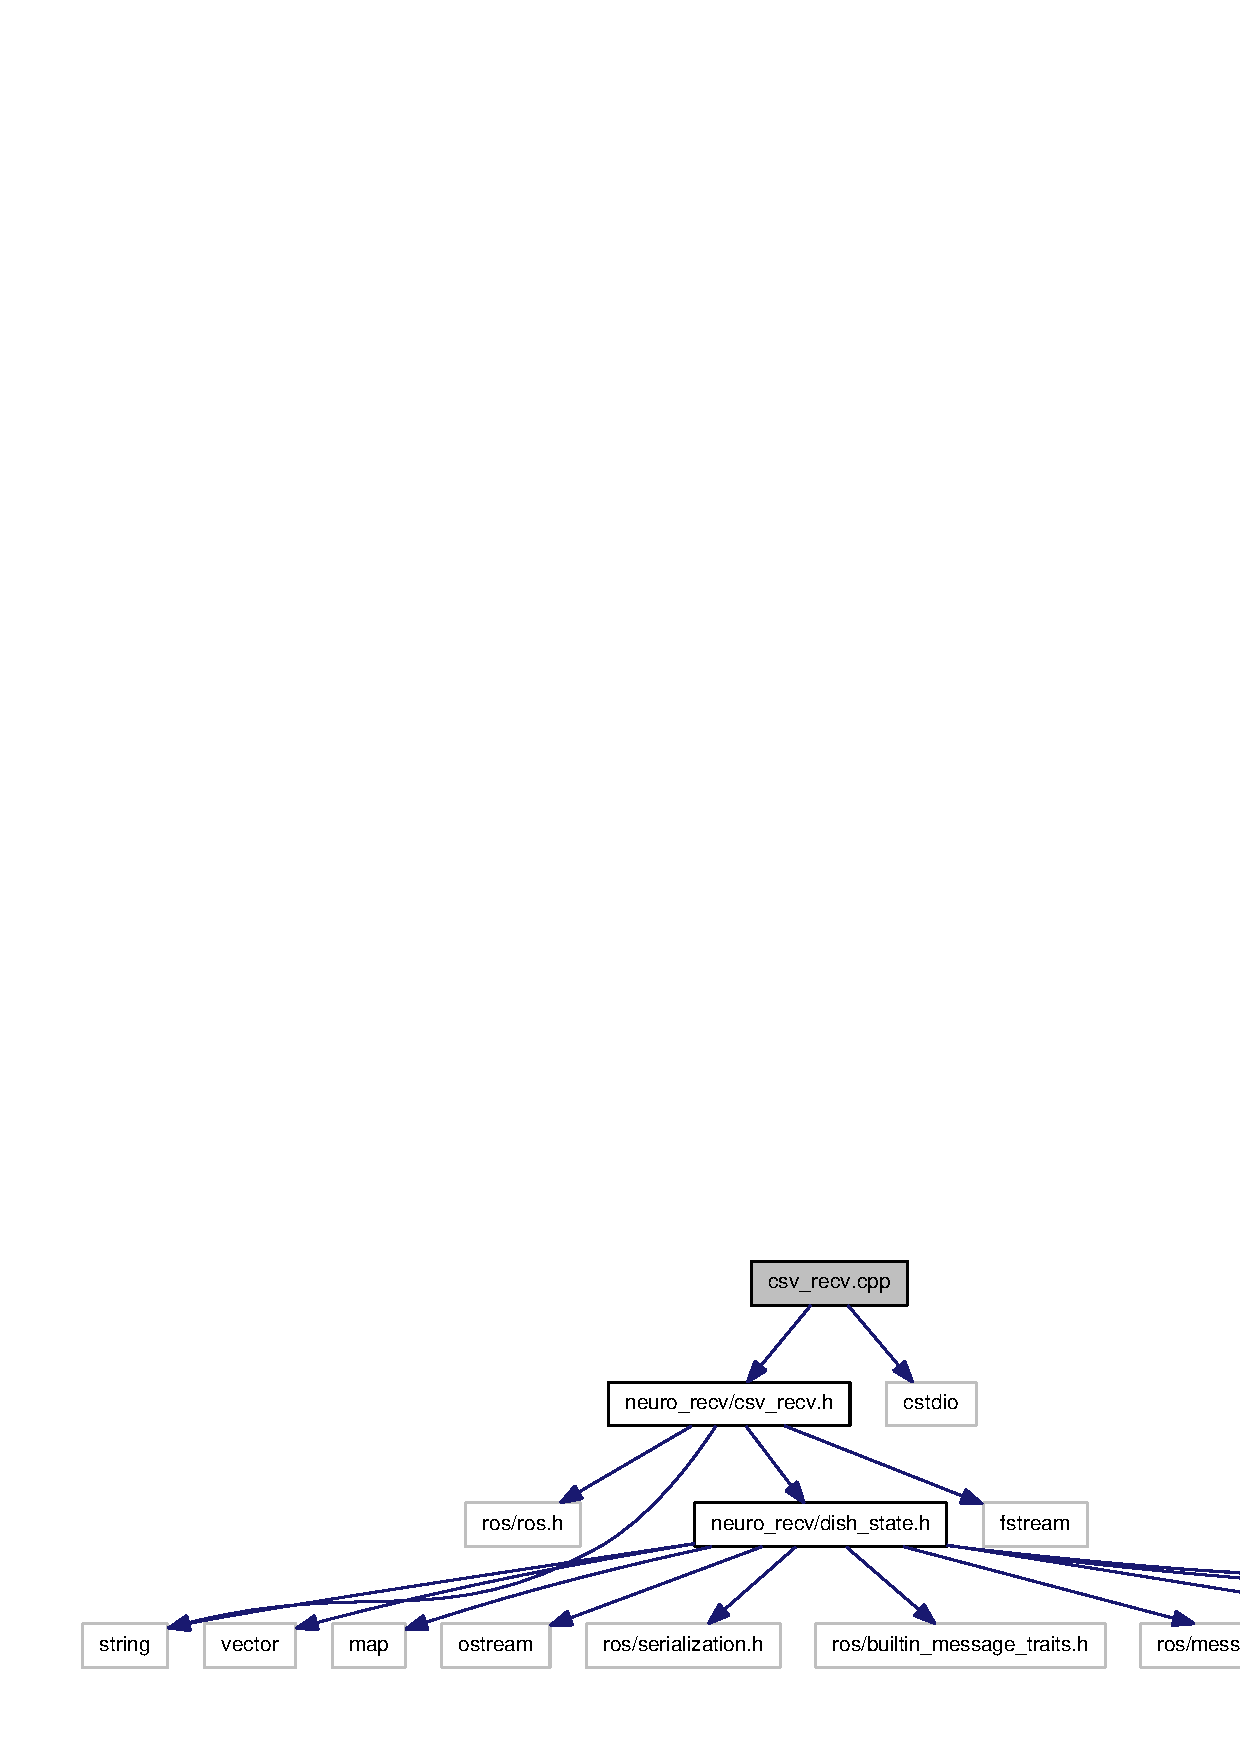
\includegraphics[width=350pt]{csv__recv_8cpp__incl}
\end{center}
\end{figure}
\subsection*{\-Functions}
\begin{DoxyCompactItemize}
\item 
int {\bf main} (int argc, char $\ast$$\ast$argv)
\begin{DoxyCompactList}\small\item\em \-Creates an instance of the node. \end{DoxyCompactList}\end{DoxyCompactItemize}


\subsection{\-Function \-Documentation}
\index{csv\-\_\-recv.\-cpp@{csv\-\_\-recv.\-cpp}!main@{main}}
\index{main@{main}!csv_recv.cpp@{csv\-\_\-recv.\-cpp}}
\subsubsection[{main}]{\setlength{\rightskip}{0pt plus 5cm}int {\bf main} (
\begin{DoxyParamCaption}
\item[{int}]{argc, }
\item[{char $\ast$$\ast$}]{argv}
\end{DoxyParamCaption}
)}\label{csv__recv_8cpp_a3c04138a5bfe5d72780bb7e82a18e627}


\-Creates an instance of the node. 



\-Definition at line 245 of file csv\-\_\-recv.\-cpp.


\section{csv\-\_\-recv.\-h \-File \-Reference}
\label{csv__recv_8h}\index{csv\-\_\-recv.\-h@{csv\-\_\-recv.\-h}}
{\ttfamily \#include \char`\"{}ros/ros.\-h\char`\"{}}\*
{\ttfamily \#include \char`\"{}neuro\-\_\-recv/dish\-\_\-state.\-h\char`\"{}}\*
{\ttfamily \#include $<$string$>$}\*
{\ttfamily \#include $<$fstream$>$}\*
\-Include dependency graph for csv\-\_\-recv.\-h\-:\nopagebreak
\begin{figure}[H]
\begin{center}
\leavevmode
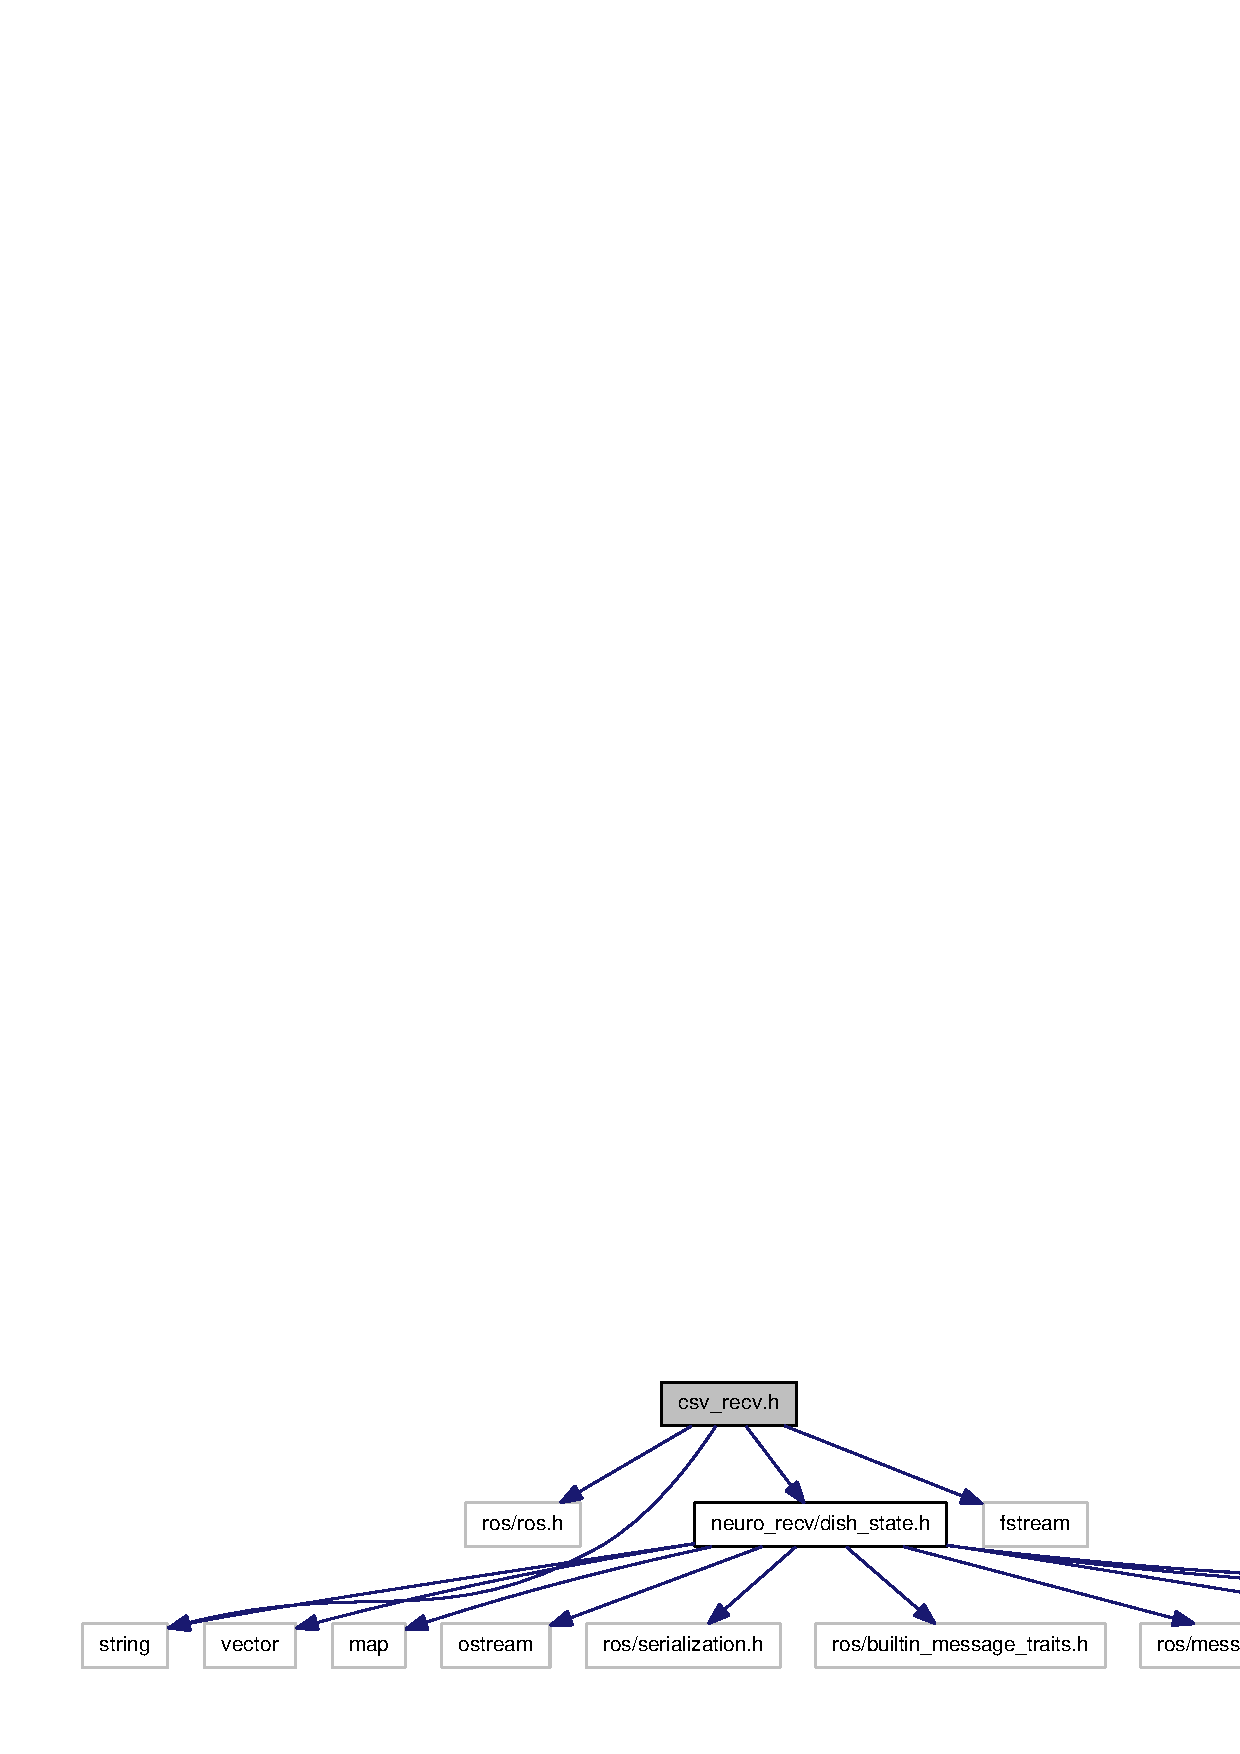
\includegraphics[width=350pt]{csv__recv_8h__incl}
\end{center}
\end{figure}
\-This graph shows which files directly or indirectly include this file\-:\nopagebreak
\begin{figure}[H]
\begin{center}
\leavevmode
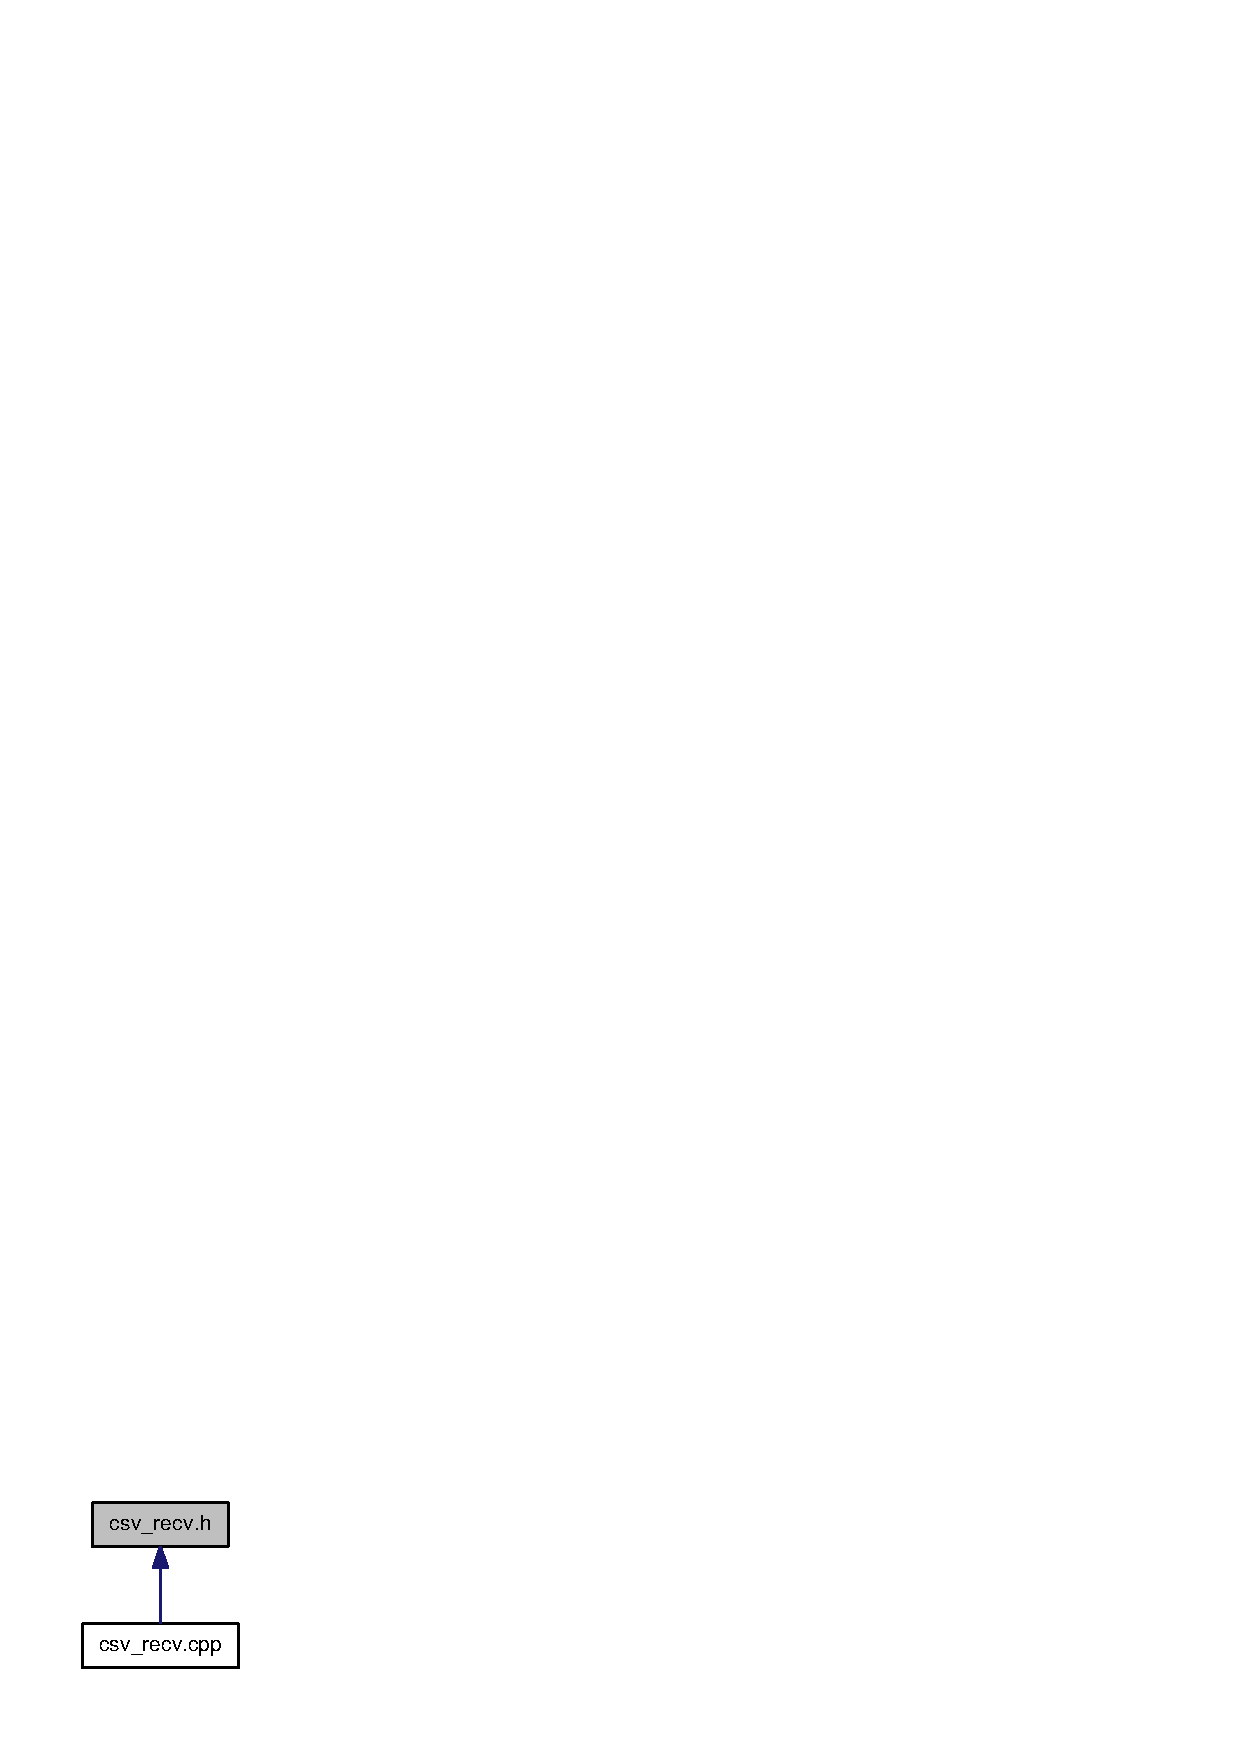
\includegraphics[width=118pt]{csv__recv_8h__dep__incl}
\end{center}
\end{figure}
\subsection*{\-Classes}
\begin{DoxyCompactItemize}
\item 
class {\bf \-Csv\-Receiver}
\begin{DoxyCompactList}\small\item\em \-Node for publishing dish states from a \-C\-S\-V file. \end{DoxyCompactList}\end{DoxyCompactItemize}

\section{dish\-\_\-generator.\-cpp \-File \-Reference}
\label{dish__generator_8cpp}\index{dish\-\_\-generator.\-cpp@{dish\-\_\-generator.\-cpp}}
{\ttfamily \#include \char`\"{}ros/ros.\-h\char`\"{}}\*
{\ttfamily \#include \char`\"{}neuro\-\_\-recv/dish\-\_\-state.\-h\char`\"{}}\*
{\ttfamily \#include $<$cstdlib$>$}\*
{\ttfamily \#include $<$cstdio$>$}\*
{\ttfamily \#include $<$ctime$>$}\*
{\ttfamily \#include $<$cmath$>$}\*
\-Include dependency graph for dish\-\_\-generator.\-cpp\-:\nopagebreak
\begin{figure}[H]
\begin{center}
\leavevmode
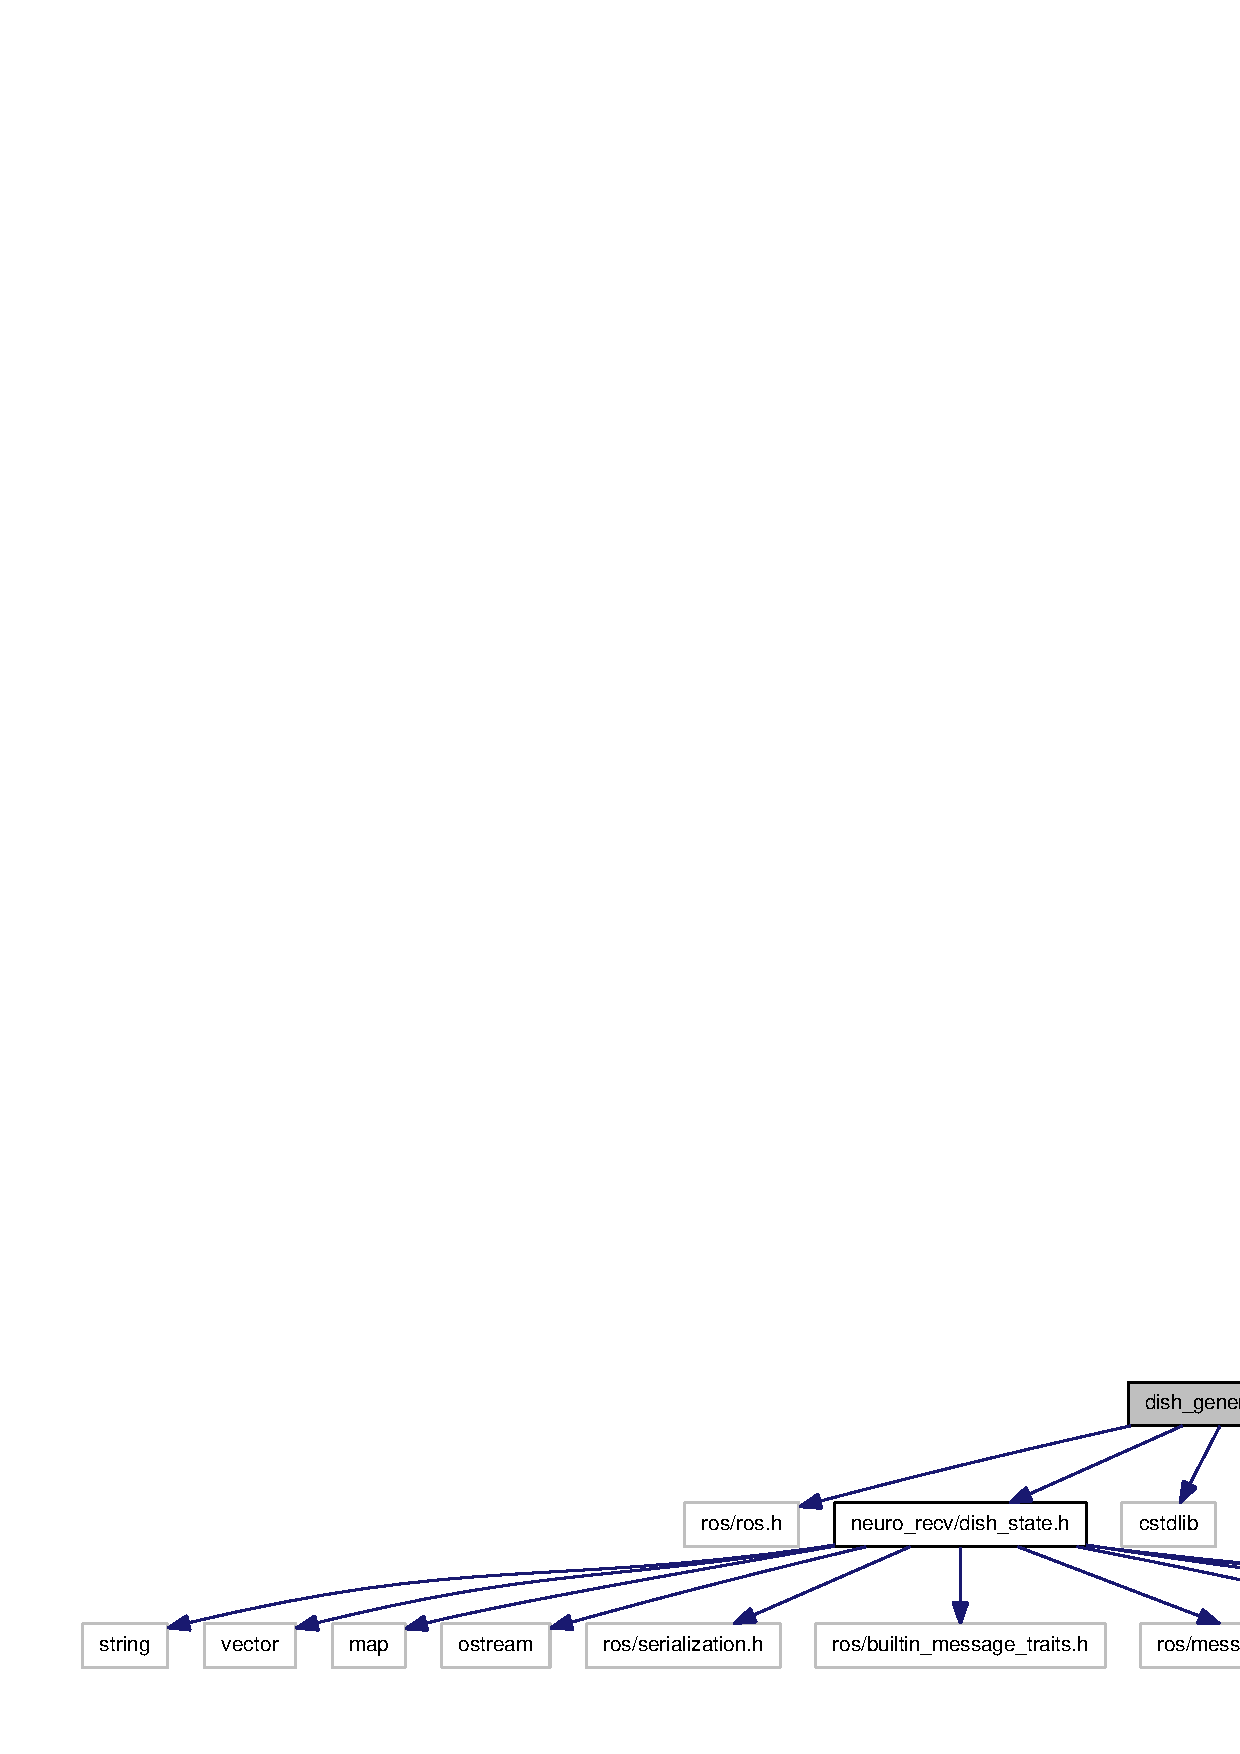
\includegraphics[width=350pt]{dish__generator_8cpp__incl}
\end{center}
\end{figure}
\subsection*{\-Defines}
\begin{DoxyCompactItemize}
\item 
\#define {\bf \-L\-I\-M\-I\-T}~0.\-003
\end{DoxyCompactItemize}
\subsection*{\-Functions}
\begin{DoxyCompactItemize}
\item 
int {\bf main} (int argc, char $\ast$$\ast$argv)
\begin{DoxyCompactList}\small\item\em \-Test node that generates and publishes pseudorandom dish states \begin{DoxyCopyright}{\-Copyright}
\-Copyright 2013 \-University of \-Massachusetts \-Lowell. 
\end{DoxyCopyright}
\end{DoxyCompactList}\end{DoxyCompactItemize}


\subsection{\-Define \-Documentation}
\index{dish\-\_\-generator.\-cpp@{dish\-\_\-generator.\-cpp}!\-L\-I\-M\-I\-T@{\-L\-I\-M\-I\-T}}
\index{\-L\-I\-M\-I\-T@{\-L\-I\-M\-I\-T}!dish_generator.cpp@{dish\-\_\-generator.\-cpp}}
\subsubsection[{\-L\-I\-M\-I\-T}]{\setlength{\rightskip}{0pt plus 5cm}\#define {\bf \-L\-I\-M\-I\-T}~0.\-003}\label{dish__generator_8cpp_a5977928b042d0a4b2ce93baa979e5f5c}


\-Definition at line 14 of file dish\-\_\-generator.\-cpp.



\subsection{\-Function \-Documentation}
\index{dish\-\_\-generator.\-cpp@{dish\-\_\-generator.\-cpp}!main@{main}}
\index{main@{main}!dish_generator.cpp@{dish\-\_\-generator.\-cpp}}
\subsubsection[{main}]{\setlength{\rightskip}{0pt plus 5cm}int {\bf main} (
\begin{DoxyParamCaption}
\item[{int}]{argc, }
\item[{char $\ast$$\ast$}]{argv}
\end{DoxyParamCaption}
)}\label{dish__generator_8cpp_a3c04138a5bfe5d72780bb7e82a18e627}


\-Test node that generates and publishes pseudorandom dish states \begin{DoxyCopyright}{\-Copyright}
\-Copyright 2013 \-University of \-Massachusetts \-Lowell. 
\end{DoxyCopyright}


\begin{DoxyAuthor}{\-Author}
\-Jonathan \-Hasenzahl 
\end{DoxyAuthor}


\-Definition at line 21 of file dish\-\_\-generator.\-cpp.


\section{dish\-\_\-state.\-h \-File \-Reference}
\label{dish__state_8h}\index{dish\-\_\-state.\-h@{dish\-\_\-state.\-h}}
{\ttfamily \#include $<$string$>$}\*
{\ttfamily \#include $<$vector$>$}\*
{\ttfamily \#include $<$map$>$}\*
{\ttfamily \#include $<$ostream$>$}\*
{\ttfamily \#include \char`\"{}ros/serialization.\-h\char`\"{}}\*
{\ttfamily \#include \char`\"{}ros/builtin\-\_\-message\-\_\-traits.\-h\char`\"{}}\*
{\ttfamily \#include \char`\"{}ros/message\-\_\-operations.\-h\char`\"{}}\*
{\ttfamily \#include \char`\"{}ros/time.\-h\char`\"{}}\*
{\ttfamily \#include \char`\"{}ros/macros.\-h\char`\"{}}\*
{\ttfamily \#include \char`\"{}ros/assert.\-h\char`\"{}}\*
{\ttfamily \#include \char`\"{}std\-\_\-msgs/\-Header.\-h\char`\"{}}\*
\-Include dependency graph for dish\-\_\-state.\-h\-:\nopagebreak
\begin{figure}[H]
\begin{center}
\leavevmode
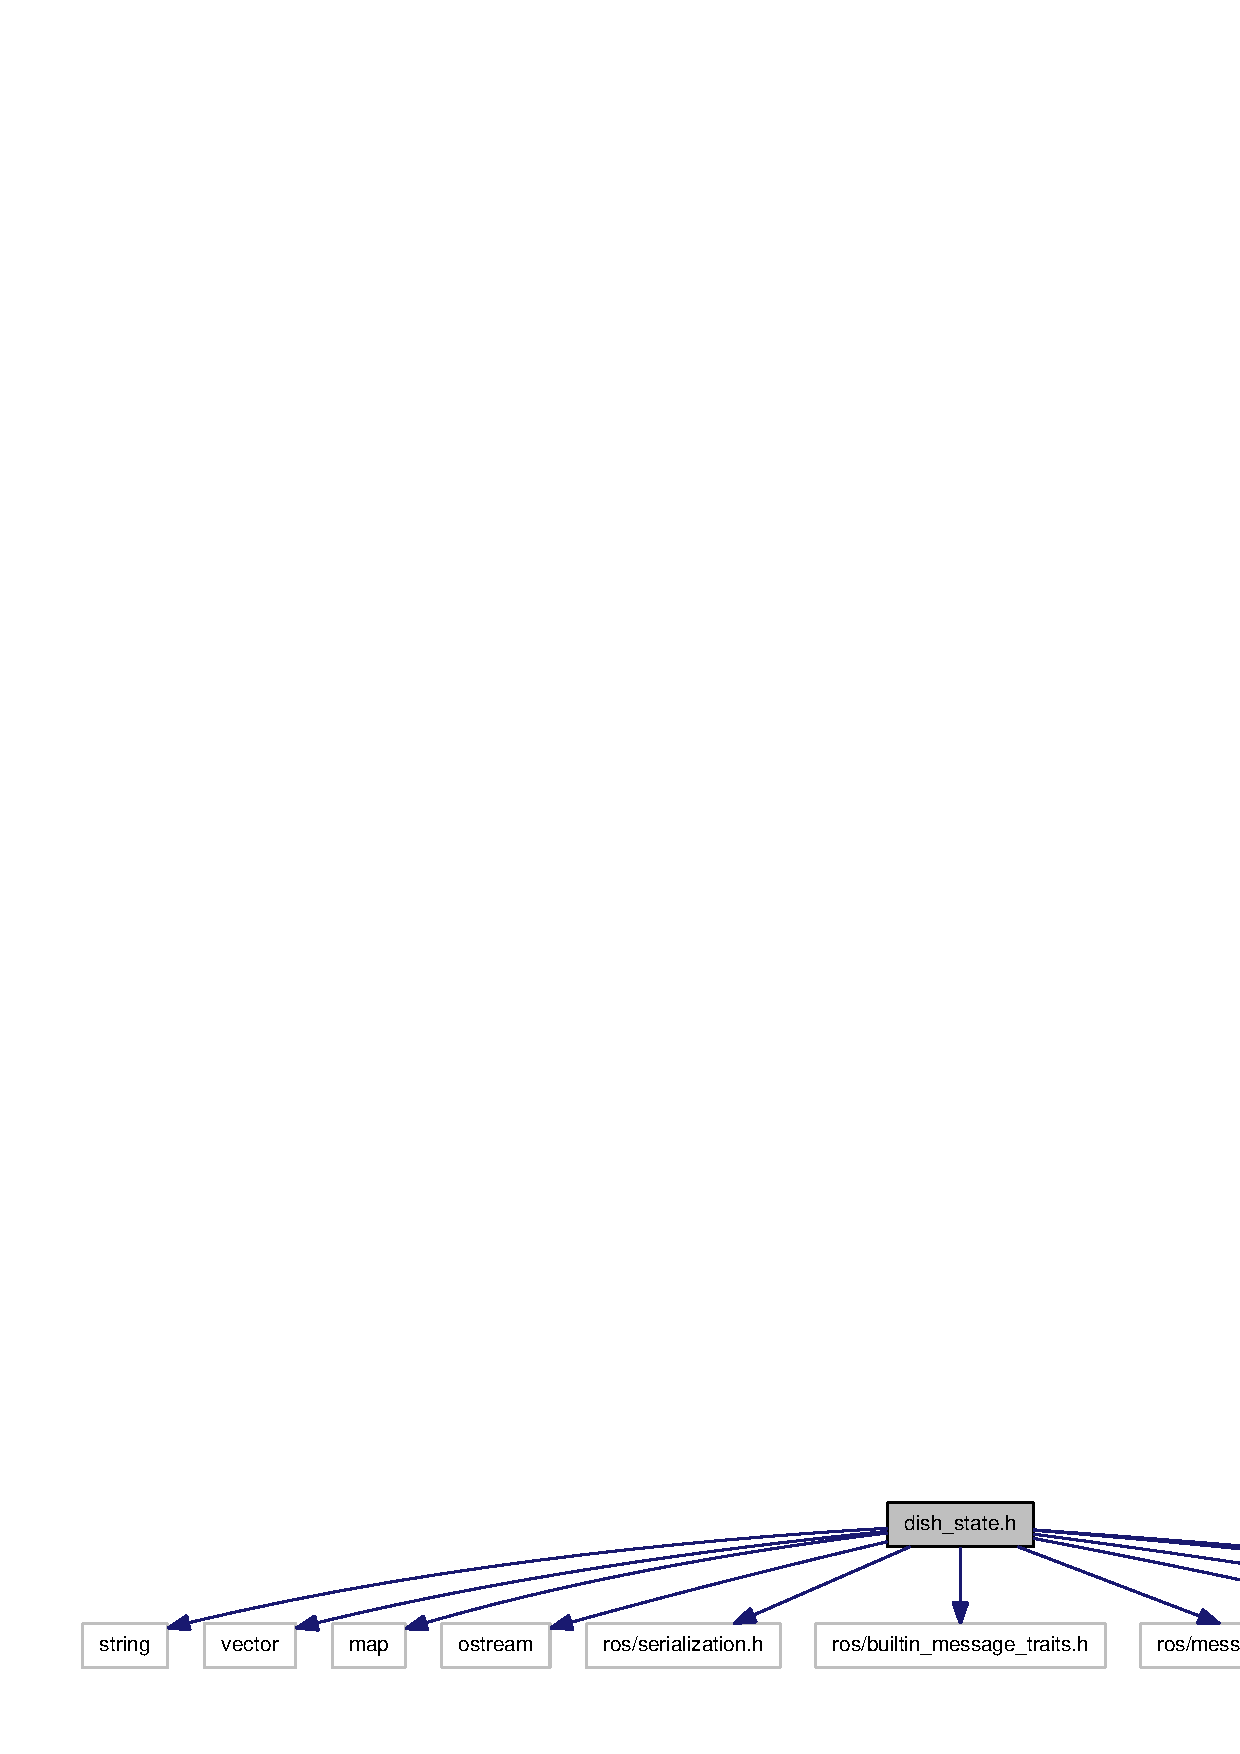
\includegraphics[width=350pt]{dish__state_8h__incl}
\end{center}
\end{figure}
\-This graph shows which files directly or indirectly include this file\-:\nopagebreak
\begin{figure}[H]
\begin{center}
\leavevmode
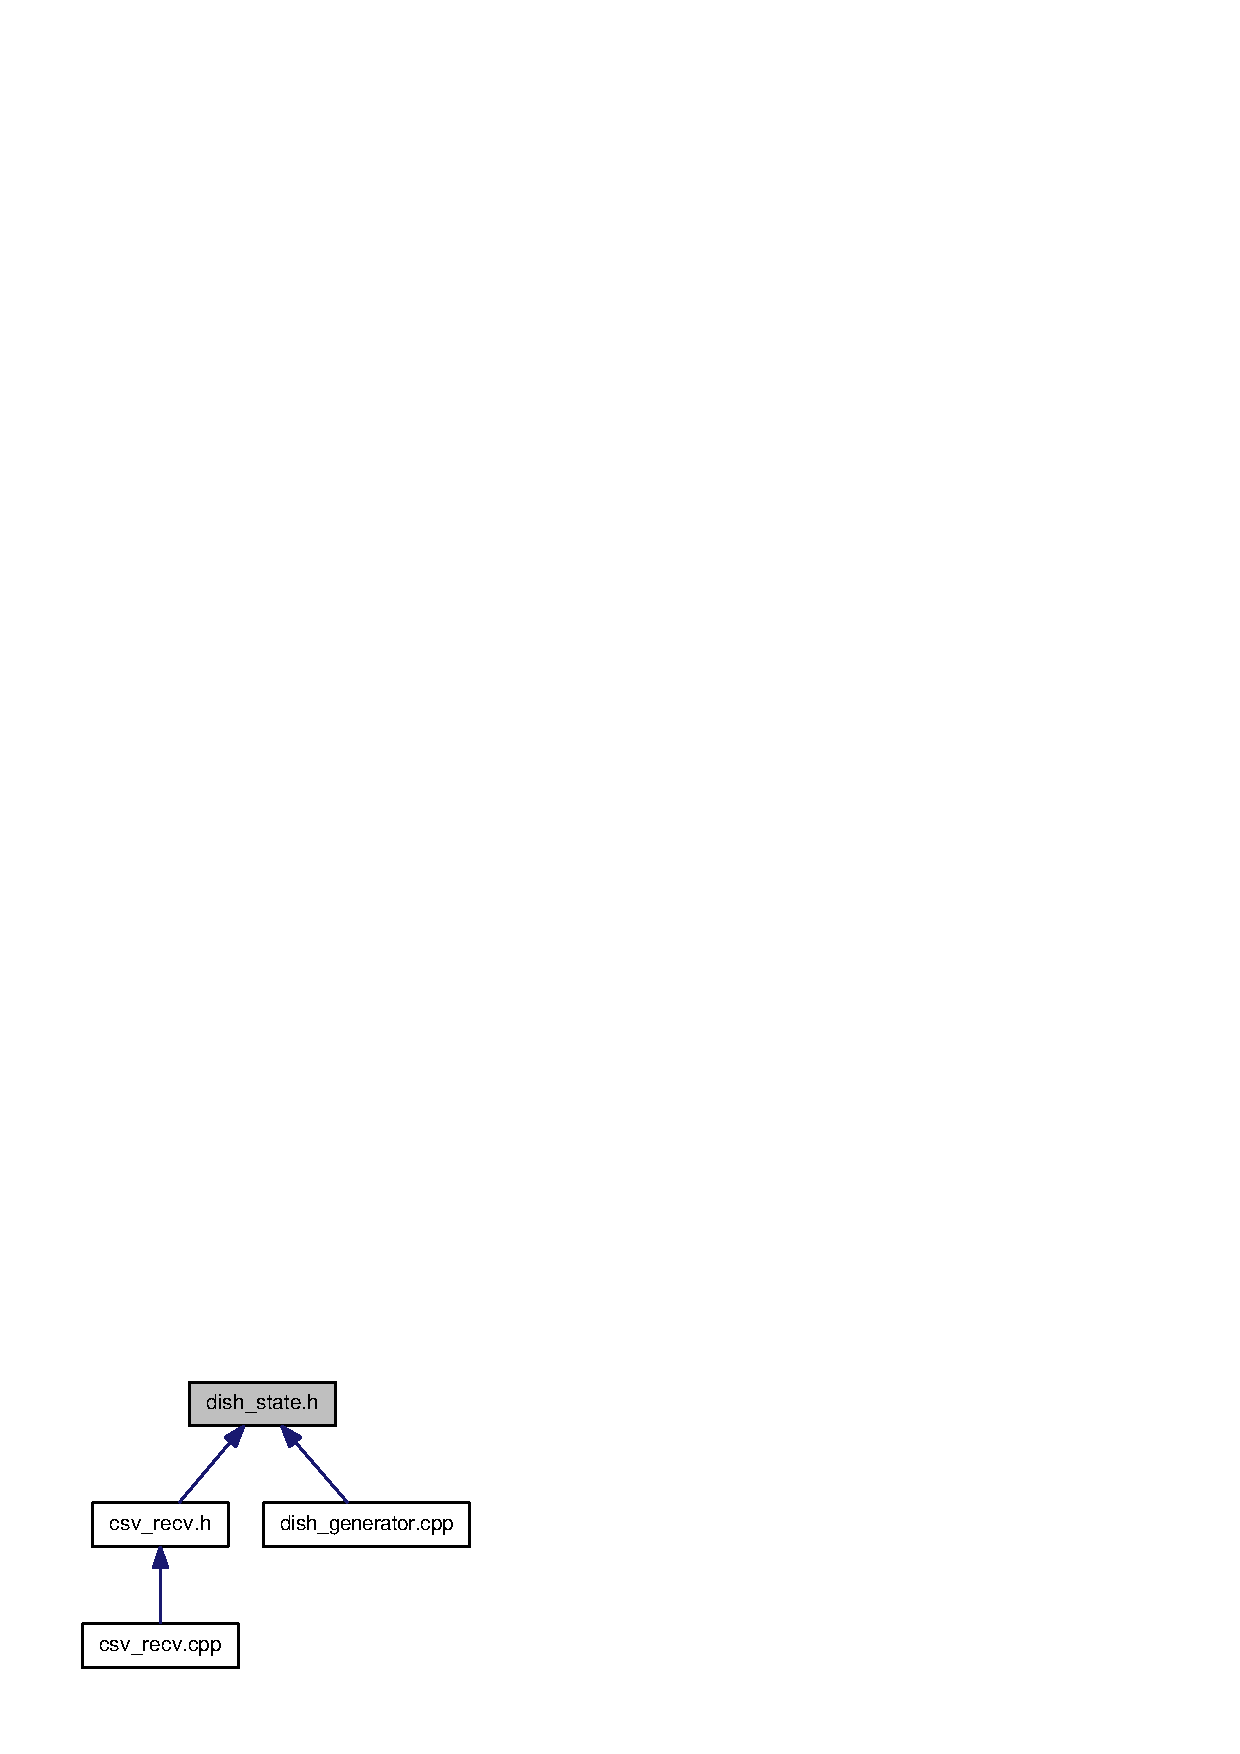
\includegraphics[width=229pt]{dish__state_8h__dep__incl}
\end{center}
\end{figure}
\subsection*{\-Classes}
\begin{DoxyCompactItemize}
\item 
struct {\bf ros\-::message\-\_\-traits\-::\-Data\-Type$<$ \-::neuro\-\_\-recv\-::dish\-\_\-state\-\_\-$<$ Container\-Allocator $>$ $>$}
\item 
struct {\bf ros\-::message\-\_\-traits\-::\-Definition$<$ \-::neuro\-\_\-recv\-::dish\-\_\-state\-\_\-$<$ Container\-Allocator $>$ $>$}
\item 
struct {\bf neuro\-\_\-recv\-::dish\-\_\-state\-\_\-$<$ Container\-Allocator $>$}
\item 
struct {\bf ros\-::message\-\_\-traits\-::\-Has\-Header$<$ \-::neuro\-\_\-recv\-::dish\-\_\-state\-\_\-$<$ Container\-Allocator $>$ $>$}
\item 
struct {\bf ros\-::message\-\_\-traits\-::\-Has\-Header$<$ const \-::neuro\-\_\-recv\-::dish\-\_\-state\-\_\-$<$ Container\-Allocator $>$ $>$}
\item 
struct {\bf ros\-::message\-\_\-traits\-::\-Is\-Message$<$ \-::neuro\-\_\-recv\-::dish\-\_\-state\-\_\-$<$ Container\-Allocator $>$ $>$}
\item 
struct {\bf ros\-::message\-\_\-traits\-::\-Is\-Message$<$ \-::neuro\-\_\-recv\-::dish\-\_\-state\-\_\-$<$ Container\-Allocator $>$const  $>$}
\item 
struct {\bf ros\-::message\-\_\-traits\-::\-M\-D5\-Sum$<$ \-::neuro\-\_\-recv\-::dish\-\_\-state\-\_\-$<$ Container\-Allocator $>$ $>$}
\item 
struct {\bf ros\-::message\-\_\-operations\-::\-Printer$<$ \-::neuro\-\_\-recv\-::dish\-\_\-state\-\_\-$<$ Container\-Allocator $>$ $>$}
\item 
struct {\bf ros\-::serialization\-::\-Serializer$<$ \-::neuro\-\_\-recv\-::dish\-\_\-state\-\_\-$<$ Container\-Allocator $>$ $>$}
\end{DoxyCompactItemize}
\subsection*{\-Namespaces}
\begin{DoxyCompactItemize}
\item 
namespace {\bf neuro\-\_\-recv}
\item 
namespace {\bf ros}
\item 
namespace {\bf ros\-::message\-\_\-operations}
\item 
namespace {\bf ros\-::message\-\_\-traits}
\item 
namespace {\bf ros\-::serialization}
\end{DoxyCompactItemize}
\subsection*{\-Typedefs}
\begin{DoxyCompactItemize}
\item 
typedef \*
\-::{\bf neuro\-\_\-recv\-::dish\-\_\-state\-\_\-}\*
$<$ std\-::allocator$<$ void $>$ $>$ {\bf neuro\-\_\-recv\-::dish\-\_\-state}
\item 
typedef boost\-::shared\-\_\-ptr\*
$<$ \-::{\bf neuro\-\_\-recv\-::dish\-\_\-state} \*
const  $>$ {\bf neuro\-\_\-recv\-::dish\-\_\-state\-Const\-Ptr}
\item 
typedef boost\-::shared\-\_\-ptr\*
$<$ \-::{\bf neuro\-\_\-recv\-::dish\-\_\-state} $>$ {\bf neuro\-\_\-recv\-::dish\-\_\-state\-Ptr}
\end{DoxyCompactItemize}
\subsection*{\-Functions}
\begin{DoxyCompactItemize}
\item 
{\footnotesize template$<$typename Container\-Allocator $>$ }\\std\-::ostream \& {\bf neuro\-\_\-recv\-::operator$<$$<$} (std\-::ostream \&s, const \-::{\bf neuro\-\_\-recv\-::dish\-\_\-state\-\_\-}$<$ \-Container\-Allocator $>$ \&v)
\end{DoxyCompactItemize}

\section{mainpage.\-dox \-File \-Reference}
\label{mainpage_8dox}\index{mainpage.\-dox@{mainpage.\-dox}}

\section{\-Seed\-Mea.\-py \-File \-Reference}
\label{SeedMea_8py}\index{\-Seed\-Mea.\-py@{\-Seed\-Mea.\-py}}
\subsection*{\-Classes}
\begin{DoxyCompactItemize}
\item 
class {\bf \-Seed\-Mea.\-Channel}
\begin{DoxyCompactList}\small\item\em \-Data structure for a \-M\-E\-A channel pad neurons\-: list of neurons within range of the pad total\-\_\-weight\-: combined weights of all the neurons. \end{DoxyCompactList}\item 
class {\bf \-Seed\-Mea.\-Close\-Neuron}
\begin{DoxyCompactList}\small\item\em \-Data structure for a neuron that is close to a channel pad. \end{DoxyCompactList}\end{DoxyCompactItemize}
\subsection*{\-Namespaces}
\begin{DoxyCompactItemize}
\item 
namespace {\bf \-Seed\-Mea}
\begin{DoxyCompactList}\small\item\em \-This is a \-R\-O\-S node that is used by itself to generate network connectivity pickle files for the \doxyref{brian\-\_\-recv.\-py}{p.}{brian__recv_8py} and \doxyref{brian\-\_\-to\-\_\-csv.\-py}{p.}{brian__to__csv_8py} nodes. \end{DoxyCompactList}\end{DoxyCompactItemize}
\subsection*{\-Functions}
\begin{DoxyCompactItemize}
\item 
def {\bf \-Seed\-Mea.\-count\-Cells}
\item 
def {\bf \-Seed\-Mea.\-density\-Reap}
\item 
def {\bf \-Seed\-Mea.\-displace}
\item 
def {\bf \-Seed\-Mea.\-di\-Sq\-Plasma}
\item 
def {\bf \-Seed\-Mea.\-gauss\-Connect}
\begin{DoxyCompactList}\small\item\em \-Calculate the probability of a connection between two neurons, based on their distance apart. \end{DoxyCompactList}\item 
def {\bf \-Seed\-Mea.\-gen\-P\-Cell}
\begin{DoxyCompactList}\small\item\em \-Takes a 2-\/\-D \-Numpy array and fill it in with a density map. \end{DoxyCompactList}\item 
def {\bf \-Seed\-Mea.\-grim\-Reap}
\item 
def {\bf \-Seed\-Mea.\-next\-Pow\-Two}
\begin{DoxyCompactList}\small\item\em \-Find the next highest power of two, to get a shape that's good for plasma fractal generation. \end{DoxyCompactList}\item 
def {\bf \-Seed\-Mea.\-render\-Map}
\begin{DoxyCompactList}\small\item\em \-Use pygame to render an array. \end{DoxyCompactList}\item 
def {\bf \-Seed\-Mea.\-square\-Plasma}
\end{DoxyCompactItemize}
\subsection*{\-Variables}
\begin{DoxyCompactItemize}
\item 
int {\bf \-Seed\-Mea.\-axon\-\_\-growth} = 220
\item 
{\bf \-Seed\-Mea.\-axon\-\_\-max} = dish\-\_\-width
\item 
tuple {\bf \-Seed\-Mea.\-Ce} = \-Connection(\-P, \-P, 'ge')
\item 
int {\bf \-Seed\-Mea.\-cell\-\_\-density} = 900
\item 
tuple {\bf \-Seed\-Mea.\-cells\-\_\-per\-\_\-edge} = int(dish\-\_\-width/soma\-\_\-dia)
\item 
tuple {\bf \-Seed\-Mea.\-Ci} = \-Connection(\-P, \-P, 'gi')
\item 
tuple {\bf \-Seed\-Mea.\-close\-\_\-neurons} = \-Channel()
\item 
tuple {\bf \-Seed\-Mea.\-conn\-\_\-graph} = nx.\-Di\-Graph()
\item 
list {\bf \-Seed\-Mea.\-conn\-\_\-list} = [$\,$]
\item 
int {\bf \-Seed\-Mea.\-connectivity\-\_\-rate} = 55
\item 
int {\bf \-Seed\-Mea.\-dendrite\-\_\-max} = 180
\item 
tuple {\bf \-Seed\-Mea.\-density\-\_\-map} = np.\-zeros((edge\-\_\-len, edge\-\_\-len))
\item 
int {\bf \-Seed\-Mea.\-dish\-\_\-width} = 2500
\item 
tuple {\bf \-Seed\-Mea.\-dist} = math.\-sqrt((neuron\-\_\-x\-\_\-loc -\/ pad\-\_\-x\-\_\-loc)$\ast$$\ast$2 + (neuron\-\_\-y\-\_\-loc -\/ pad\-\_\-y\-\_\-loc)$\ast$$\ast$2)
\item 
tuple {\bf \-Seed\-Mea.\-distance} = math.\-sqrt((from\-\_\-neuron[0][0] -\/ to\-\_\-neuron[0][0])$\ast$$\ast$2 + (from\-\_\-neuron[0][1] -\/ to\-\_\-neuron[0][1])$\ast$$\ast$2)
\item 
tuple {\bf \-Seed\-Mea.\-edge\-\_\-len} = next\-Pow\-Two(cells\-\_\-per\-\_\-edge)
\item 
string {\bf \-Seed\-Mea.\-eqs}
\item 
tuple {\bf \-Seed\-Mea.\-excitory\-\_\-count} = int(neuron\-\_\-count $\ast$ 0.\-75)
\item 
tuple {\bf \-Seed\-Mea.\-expected\-\_\-cells} = (dish\-\_\-width/1000)
\item 
string {\bf \-Seed\-Mea.\-file\-\_\-date} = \char`\"{}\{0\}-\/\{1\}-\/\{2\}-\/\{3\}\-:\{4\}\-:\{5\}\char`\"{}
\item 
{\bf \-Seed\-Mea.\-ignore\-\_\-corners} = \-True
\item 
{\bf \-Seed\-Mea.\-inhib\-\_\-count} = neuron\-\_\-count-\/excitory\-\_\-count
\item 
tuple {\bf \-Seed\-Mea.\-inhib\-\_\-neurons} = random.\-sample(xrange(neuron\-\_\-count), inhib\-\_\-count)
\item 
tuple {\bf \-Seed\-Mea.\-neuron\-\_\-count} = int(count\-Cells(density\-\_\-map))
\item 
int {\bf \-Seed\-Mea.\-neuron\-\_\-id} = 0
\item 
list {\bf \-Seed\-Mea.\-neuron\-\_\-list} = [$\,$]
\item 
list {\bf \-Seed\-Mea.\-neuron\-\_\-x\-\_\-loc} = neuron[0]
\item 
list {\bf \-Seed\-Mea.\-neuron\-\_\-y\-\_\-loc} = neuron[0]
\item 
tuple {\bf \-Seed\-Mea.\-now} = datetime.\-datetime.\-now()
\item 
tuple {\bf \-Seed\-Mea.\-P} = \-Neuron\-Group(neuron\-\_\-count, eqs, threshold=-\/50$\ast$m\-V, reset=-\/60$\ast$m\-V)
\item 
int {\bf \-Seed\-Mea.\-pad\-\_\-cols} = 8
\item 
int {\bf \-Seed\-Mea.\-pad\-\_\-dia} = 30
\item 
dictionary {\bf \-Seed\-Mea.\-pad\-\_\-neuron\-\_\-map} = \{\}
\item 
int {\bf \-Seed\-Mea.\-pad\-\_\-rows} = 8
\item 
int {\bf \-Seed\-Mea.\-pad\-\_\-spacing} = 200
\item 
int {\bf \-Seed\-Mea.\-pad\-\_\-threshold} = 40
\item 
{\bf \-Seed\-Mea.\-pad\-\_\-x\-\_\-loc} = pad\-\_\-x$\ast$pad\-\_\-spacing
\item 
{\bf \-Seed\-Mea.\-pad\-\_\-y\-\_\-loc} = pad\-\_\-y$\ast$pad\-\_\-spacing
\item 
int {\bf \-Seed\-Mea.\-soma\-\_\-dia} = 30
\item 
int {\bf \-Seed\-Mea.\-survival\-\_\-rate} = 65
\end{DoxyCompactItemize}

\printindex
\end{document}
